\documentclass[leqno,12pt,twoside,a4paper]{report}

% Select encoding of your inputs
\usepackage[utf8]{inputenc}

% Make latex understand and use the typographic
% rules of the language used in the document.
\usepackage[english]{babel}

% Use the vector font Latin Modern which is going
% to be the default font in latex in the future.
\usepackage{lmodern}

% Choose the font encoding
\usepackage[T1]{fontenc}

% Use color in tables
\usepackage[table]{xcolor}
\usepackage{array}
\usepackage{multirow}

% Load a colour package
\usepackage{xcolor}
\definecolor{aaublue}{RGB}{33,26,82}  %<--define aaublue
\definecolor{white}{RGB}{255,255,255} %<--define white

% The standard graphics inclusion package
\usepackage{graphicx}

\makeatletter
  \g@addto@macro\@floatboxreset\centering %<--centering all figures
\makeatother

\usepackage{adjustbox}

% Set up how figure and table captions are displayed
\usepackage{float}
\usepackage{caption}
\usepackage{subcaption}
\captionsetup
{
  justification = centering,    %<--centering caption with multiple lines
  font          = footnotesize, %<--set font size to footnotesize
  labelfont     = bf,           %<--bold label (e.g., Figure 3.2) font
  belowskip     = -15pt
}
\captionsetup[subfigure]
{
  justification = centering, %<--centering subfigure caption text
  singlelinecheck=false,
  font = footnotesize        %<--font size for subfigures
} 

% Enable row combination in tables
\usepackage{multirow}

% Make space between table lines and text
\renewcommand{\arraystretch}{1.5}

% Enable commands like \st (strike out) and \hl (high light)
\usepackage{soul}

% Make the standard latex tables look so much better
\usepackage{array,booktabs}

% Enable the use of frames around, e.g., theorems
% The framed package is used in the example environment
\usepackage{framed}
\usepackage{colortbl}
\usepackage{longtable}
\usepackage{xcolor}
\usepackage{textcomp}

%-------MATHEMATICS---------------------------------
% Defines new environments such as equation,
% align and split 
\usepackage{amsmath}
\usepackage{relsize}
% Adds new math symbols
\usepackage{amssymb}
% Use theorems in your document
% The ntheorem package is also used for the example environment
% When using thmmarks, amsmath must be an option as well. Otherwise \eqref doesn't work anymore.
\usepackage[framed,amsmath,thmmarks]{ntheorem}
\usepackage{xifthen}%<--enables ifthenelse which is used in macros

\usepackage{siunitx} 
\sisetup{decimalsymbol=period}%<--\num{} will swich commas with periods
\sisetup{detect-weight}
%---------------------------------------------------

%-------PAGE LAYOUT---------------------------------
% Change margins, papersize, etc of the document
\usepackage[
  left=25mm,% left margin on an odd page %tidligere 25mm for baade right og left
  right=25mm,% right margin on an odd page
  top=35mm,
  ]{geometry}

%break margins when you need to on only part of a page if needed
\usepackage{changepage}
%syntax
% \begin{adjustwidth}{-1.2cm}{-1.2cm}
%    [ big object ]
% \end{adjustwidth}

% Modify how \chapter, \section, etc. look
% The titlesec package is very configureable
\usepackage{titlesec}
\makeatletter
\def\ttl@mkchap@i#1#2#3#4#5#6#7{%
    \ttl@assign\@tempskipa#3\relax\beforetitleunit
    \vspace{\@tempskipa}%<<<<<< REMOVE THE * AFTER \vspace
    \global\@afterindenttrue
    \ifcase#5 \global\@afterindentfalse\fi
    \ttl@assign\@tempskipb#4\relax\aftertitleunit
    \ttl@topmode{\@tempskipb}{%
        \ttl@select{#6}{#1}{#2}{#7}}%
    \ttl@finmarks  % Outside the box!
    \@ifundefined{ttlp@#6}{}{\ttlp@write{#6}}}
\makeatother

\titlespacing{\chapter}{0pt}{0pt}{10pt}
\titlespacing{\section}{0pt}{0pt}{-5pt}
\titlespacing{\subsection}{0pt}{8pt}{-5pt}
\titlespacing{\subsubsection}{0pt}{6pt}{-10pt}

\titleformat*{\section}{\normalfont\Large\bfseries\color{aaublue}}
\titleformat*{\subsection}{\normalfont\large\bfseries\color{aaublue}}
\titleformat*{\subsubsection}{\normalfont\normalsize\bfseries\color{aaublue}}

\usepackage{titlesec, blindtext, color}
%\color{gray75}{gray}{0.75}
\newcommand{\hsp}{\hspace{20pt}}
\titleformat{\chapter}[hang]{\Huge\bfseries}{\thechapter\hsp\textcolor{aaublue}{|}\hsp}{0pt}{\Huge\bfseries}

% Change the headers and footers
\usepackage{fancyhdr}
\setlength{\headheight}{15pt}
\pagestyle{fancy}
\fancyhf{} %delete everything
\renewcommand{\headrulewidth}{0pt} %remove the horizontal line in the header
\fancyhead[RO,LE]{\color{aaublue}\small\nouppercase\leftmark} %even page - chapter title
\fancyhead[LO]{}
\fancyhead[RE]{} 
\fancyhead[CE]{}
\fancyhead[CO]{}
\fancyfoot[RE,LO]{\thepage}
\fancyfoot[LE,RO]{} %page number on all pages
\fancyfoot[CE,CO]{}

% change first page of all chapters header and footer to fancy style
\makeatletter
\let\ps@plain\ps@fancy
\makeatother

% Do not stretch the content of a page. Instead,
% insert white space at the bottom of the page
\raggedbottom

% Enable arithmetics with length. Useful when typesetting the layout.
\usepackage{calc}
%---------------------------------------------------

%-------BIBLIOGRAPHY--------------------------------
%setting references (using numbers) and supporting i.a. Chicargo-style:
\usepackage{etex}
\usepackage{etoolbox}
\usepackage{keyval}
\usepackage{ifthen}
\usepackage{url}
\usepackage{csquotes}
\usepackage[backend=biber, url=true, doi=true, style=numeric, sorting=none]{biblatex}
\addbibresource{setup/bibliography.bib}
%---------------------------------------------------

%-------MISC----------------------------------------
%%% Enables the use FiXme refferences. Syntax: \fxnote{...} %%%
\usepackage[footnote, draft, english, silent, nomargin]{fixme}
%With "final" instead of "draft" an error will ocure for every FiXme under compilation.

%%% allows use of lorem ipsum (generate i.e. pagagraph 1 to 5 with \lipsum[1-5]) %%%
\usepackage{lipsum}

%%% Enables figures with text wrapped tightly around it %%%
\usepackage{wrapfig}

%%% Enable use of dashed lines in tables ( \hdashline )
\usepackage{arydshln}

%%% Section debth included in table of contents (1 = down to sections) %%%
\setcounter{tocdepth}{1}

%%% Section debth for numbers (1 = down to sections) %%%
\setcounter{secnumdepth}{1}

\usepackage{tocloft}
\setlength{\cftbeforetoctitleskip}{0 cm}
\renewcommand{\cftpartpresnum}{Part~}
\let\cftoldpartfont\cftpartfont
\renewcommand{\cftpartfont}{\cftoldpartfont\cftpartpresnum}
%---------------------------------------------------

%-------HYPERLINKS----------------------------------
% Enable hyperlinks and insert info into the pdf
% file. Hypperref should be loaded as one of the 
% last packages
\usepackage{nameref}
\usepackage{hyperref}
\usepackage{bookmark}
\hypersetup{%
	%pdfpagelabels=true,%
	plainpages=false,%
	pdfauthor={Author(s)},%
	pdftitle={Title},%
	pdfsubject={Subject},%
	bookmarksnumbered=true,%
	colorlinks,%
	citecolor=aaublue,%
	filecolor=aaublue,%
	linkcolor=aaublue,% you should probably change this to black before printing
	urlcolor=aaublue,%
	pdfstartview=FitH%
}
%---------------------------------------------------

% remove all indentations
\setlength\parindent{0pt}
\parskip 5mm
\usepackage{verbatim}

\definecolor{Gra}{RGB}{230,230,230}

%creates a nice-looking C#-text
\newcommand{\CC}{C\nolinebreak\hspace{-.05em}\raisebox{.3ex}{\scriptsize\text \#} }

%enables multi column lists
\usepackage{multicol}

%enables code-examples
\usepackage{listings}

\definecolor{coolblue}{RGB}{32,95,128}
\definecolor{mygreen}{rgb}{0,0.6,0}
\definecolor{mygray}{rgb}{0.5,0.5,0.5}
\definecolor{mymauve}{rgb}{0.58,0,0.82}
\usepackage{textcomp}
\definecolor{listinggray}{gray}{0.9}
\definecolor{lbcolor}{rgb}{0.9,0.9,0.9}

%for c code
\lstdefinestyle{cstyle}{
  backgroundcolor=\color{lbcolor},
	tabsize=4,
	rulecolor=,
	language=C,
  basicstyle=\scriptsize,
  upquote=true,
  aboveskip={1.5\baselineskip},
  columns=fixed,
  showstringspaces=false,
  extendedchars=true,
  breaklines=true,
  prebreak = \raisebox{0ex}[0ex][0ex]{\ensuremath{\hookleftarrow}},
  frame=single,
  showtabs=false,
  numbers=left,
  captionpos=b,
  numbersep=5pt,
  numberstyle=\tiny\color{mygray},
  showspaces=false,
  showstringspaces=false,
  identifierstyle=\ttfamily,
  keywordstyle=\color[rgb]{0,0,1},
  commentstyle=\color[rgb]{0.133,0.545,0.133},
  stringstyle=\color[rgb]{0.627,0.126,0.941},
}
%for python code
\lstdefinestyle{pythonstyle}{
    backgroundcolor=\color{lbcolor},
    tabsize=4,
    rulecolor=,
    language=python,
    basicstyle=\scriptsize,
    upquote=true,
    aboveskip={1.5\baselineskip},
    columns=fixed,
    showstringspaces=false,
    extendedchars=true,
    breaklines=true,
    prebreak = \raisebox{0ex}[0ex][0ex]{\ensuremath{\hookleftarrow}},
    frame=single,
    showtabs=false,
    numbers=left,
    captionpos=b,
    numbersep=5pt,
    numberstyle=\tiny\color{mygray},
    showspaces=false,
    showstringspaces=false,
    identifierstyle=\ttfamily,
    keywordstyle=\color[rgb]{0,0,1},
    commentstyle=\color[rgb]{0.133,0.545,0.133},
    stringstyle=\color[rgb]{0.627,0.126,0.941},
}
%for matlab code
\lstdefinestyle{matlabstyle}{
    backgroundcolor=\color{lbcolor},
    tabsize=4,
    rulecolor=,
    language=Matlab,
    basicstyle=\scriptsize,
    upquote=true,
    aboveskip={1.5\baselineskip},
    columns=fixed,
    showstringspaces=false,
    extendedchars=true,
    breaklines=true,
    prebreak = \raisebox{0ex}[0ex][0ex]{\ensuremath{\hookleftarrow}},
    frame=single,
    showtabs=false,
    numbers=left,
    captionpos=b,
    numbersep=5pt,
    numberstyle=\tiny\color{mygray},
    showspaces=false,
    showstringspaces=false,
    identifierstyle=\ttfamily,
    keywordstyle=\color[rgb]{0,0,1},
    commentstyle=\color[rgb]{0.133,0.545,0.133},
    stringstyle=\color[rgb]{0.627,0.126,0.941},   
}
%for inline c, syntax: \cline{ codeHere(); }
\lstdefinestyle{cinline}{
    style=cstyle,
    basicstyle=\small,
}
\newcommand\inlinec[1]{ \lstinline[style=cinline]{#1} }

%for inline python, syntax: \pythonline{ codeHere(); }
\lstdefinestyle{pythoninline}{
    style=pythonstyle,
    basicstyle=\small,
}
\newcommand\inlinepython[1]{ \lstinline[style=pythoninline]{#1} }

%for inline matlab, syntax: \matlabline{ codeHere(); }
\lstdefinestyle{matlabinline}{
    style=matlabstyle,
    basicstyle=\small,
}
\newcommand\inlinematlab[1]{ \lstinline[style=matlabinline]{#1} }

\usepackage{enumitem}
%\usepackage[citestyle=authoryear,natbib=true]{biblatex}

% Figures - TIKZ
\usepackage{tikz}
\usepackage[americanresistors,americaninductors,americancurrents, americanvoltages]{circuitikz}

% Wall of text logo
\newcommand{\walloftextalert}[0]{\includegraphics[width=\textwidth]{walloftext.png}}

\usepackage{pdfpages}
\usepackage{lastpage}
\usepackage{epstopdf}

\setlength{\headheight}{21pt}

\hfuzz=\maxdimen
\tolerance = 10000
\hbadness  = 10000

\usepackage{siunitx}
\graphicspath{{./figures/}}
% package inclusion and set up of the document

%this package must be included
%in a file which is open during any session
%otherwise \autoref will not autocomplete
\usepackage{hyperref}

%%%%%%%%%%%%%%%%%%%%%%%%%%%%%%%%%%%%%%%%%%%%%%%%%%%%%
%             UNITS, EQUATIONS AND TEXT             %
%%%%%%%%%%%%%%%%%%%%%%%%%%%%%%%%%%%%%%%%%%%%%%%%%%%%%

%%Macro for 'where'enviroment has been improved by Andrea :-)

%Units:
\newcommand{\unit}[1]{&& \left[\si{#1}\right]} %\newcommand{\unit}[1]{[\si{#1}]}             <<| Use these if you want equations to be
\newcommand{\unitWh}[1]{[\si{#1}]}             %\newcommand{\eq}[2]{&&\si{#1} &= \si{#2}&&}  <<| centered.. .. will appear scrambled
\newcommand{\numUnit}[1]{\ \si{#1}&}           %                                               | from one equation to the next though..
%Equation:                                     %                                               | and does not work with long equations.. :/
\newcommand{\eq}[2]{\si{#1} &= \si{#2}}
\newcommand{\arw}{&& &\Updownarrow&&}
\newcommand{\eqOne}[2]{\si{#1} &= \si{#2} &\nonumber\\}
\newcommand{\eqTwo}[1]{&\ \ \ \ \si{#1}&}
\newcommand{\eqThree}[1]{&\ \ \ \ \si{#1}&}
%Text:
\newcommand{\tx}[1]{\text{#1}}
%Vectors
\renewcommand{\vec}[1]{\boldsymbol{\mathbf{#1}}}

%Vertical line in equations ie. |_x=y (whereTwo stacks two equalities at the line)
\newcommand{\whereOne}[1]{ \left.\rule{0cm}{.7cm}\right\vert\rule{0cm}{.7cm}_{\substack{\rule{0cm}{.28cm}\\ #1 }} }
\newcommand{\whereTwo}[2]{ \left.\rule{0cm}{.7cm}\right\vert\rule{0cm}{.7cm}_{\substack{#1 \rule{0cm}{.2cm}\\\vspace{-.1cm}\\ #2}} }
\newcommand{\whereThree}[3]{ \left.\rule{0cm}{1cm}\right\vert\rule{0cm}{1cm}_{\substack{\\\vspace{-.1cm}\\ #1 \rule{0cm}{.1cm}\\\vspace{-.1cm}\\ #2 \rule{0cm}{.1cm}\\\vspace{-.1cm}\\ #3}} }





%%%%%%%%%%%%%%%%%%%%%%%%%%%%%%%%%%%%%%%%%%%%%%%%%%%%%
%              SETTING UP NOTE BOXES                %
%%%%%%%%%%%%%%%%%%%%%%%%%%%%%%%%%%%%%%%%%%%%%%%%%%%%%
%\specialcomment{note}{\[}{\]}
%%{\begin{tcolorbox}
%%                      [grow to right by  = 1.5 cm
%%                      ]}{\vspace{-.3 cm}\end{tcolorbox}}
%
%\newcommand{\toggleNotes}[1]
%{
%  \ifthenelse{\equal{#1}{off}}{\excludecomment{note}}{}
%}

%%%%%%%%%%%%%%%%%%%%%%%%%%%%%%%%%%%%%%%%%%%%%%%%%%%%%
%                 TIKZ SETTINGS                     %
%%%%%%%%%%%%%%%%%%%%%%%%%%%%%%%%%%%%%%%%%%%%%%%%%%%%%
%\usetikzlibrary{arrows.meta}
\tikzset{
  block/.style    = {draw, thick, rectangle,
                     minimum height = 2.1em,
                     minimum width = 1.7em},
  sum/.style      = {draw, circle, inner sep=1.5pt},
}

%%%%%%%%%%%%%%%%%%%%%%%%%%%%%%%%%%%%%%%%%%%%%%%%%%%%%
%                  REFERENCES                       %
%%%%%%%%%%%%%%%%%%%%%%%%%%%%%%%%%%%%%%%%%%%%%%%%%%%%%

%Chapter
\newcommand{\Chapref}[1]{\emph{Chapter \ref{#1}}}
\newcommand{\chapref}[1]{\emph{chapter \ref{#1}}}
%Section
\newcommand{\Secref}[1]{\emph{Section \ref{#1}}}
\newcommand{\secref}[1]{\emph{section \ref{#1}}}
%subSection
\newcommand{\Subsecref}[1]{\emph{Subsection \ref{#1}}}
\newcommand{\subsecref}[1]{\emph{subsection \ref{#1}}}
%Appendix
\newcommand{\Appref}[1]{\emph{Appendix \ref{#1}}}
\newcommand{\appref}[1]{\emph{appendix \ref{#1}}}
%Listings
\newcommand{\Coderef}[1]{\emph{Listings: \ref{#1}}}
\newcommand{\coderef}[1]{\emph{listings: \ref{#1}}}
%Figure:
\newcommand{\Figref}[1]{\emph{Figure \ref{#1}}}
\newcommand{\figref}[1]{\emph{figure \ref{#1}}}
%Table:
\newcommand{\Tableref}[1]{\emph{Table \ref{#1}}}
\newcommand{\tableref}[1]{\emph{table \ref{#1}}}

%Expressions:
\newcommand{\Expr}[1]{\emph{Expression (\ref{#1})}}
\newcommand{\expr}[1]{\emph{expression (\ref{#1})}}

%Equations:
%1 equation:
\newcommand{\Eqref}[1]{\emph{Equation (\ref{#1})}}
\renewcommand{\eqref}[1]{\emph{equation (\ref{#1})}}
%2 equations:
\newcommand{\EqrefTwo}[2]{\emph{Equation (\ref{#1})} and \emph{(\ref{#2})}}
\newcommand{\eqrefTwo}[2]{\emph{equation (\ref{#1})} and \emph{(\ref{#2})}}
%3 equations:
\newcommand{\EqrefThree}[3]{\emph{Equation (\ref{#1})}, \emph{(\ref{#2})} and \emph{(\ref{#3})}}
\newcommand{\eqrefThree}[3]{\emph{equation (\ref{#1})}, \emph{(\ref{#2})} and \emph{(\ref{#3})}}
%4 equations:
\newcommand{\EqrefFour}[4]{\emph{Equation (\ref{#1})}, \emph{(\ref{#2})}, \emph{(\ref{#3})} and \emph{(\ref{#4})}}
\newcommand{\eqrefFour}[4]{\emph{equation (\ref{#1})}, \emph{(\ref{#2})}, \emph{(\ref{#3})} and \emph{(\ref{#4})}}
%5 equations:
\newcommand{\EqrefFive}[5]{\emph{Equation (\ref{#1})}, \emph{(\ref{#2})}, \emph{(\ref{#3})}, \emph{(\ref{#4})} and \emph{(\ref{#5})}}
\newcommand{\eqrefFive}[5]{\emph{equation (\ref{#1})}, \emph{(\ref{#2})}, \emph{(\ref{#3})}, \emph{(\ref{#4})} and \emph{(\ref{#5})}}
%6 equations:
\newcommand{\EqrefSix}[6]{\emph{Equation (\ref{#1})}, \emph{(\ref{#2})}, \emph{(\ref{#3})}, \emph{(\ref{#4})}, \emph{(\ref{#5})} and \emph{(\ref{#6})}}
\newcommand{\eqrefSix}[6]{\emph{equation (\ref{#1})}, \emph{(\ref{#2})}, \emph{(\ref{#3})}, \emph{(\ref{#4})}, \emph{(\ref{#5})} and \emph{(\ref{#6})}}
%7 equations:
\newcommand{\EqrefSeven}[7]{\emph{Equation (\ref{#1})}, \emph{(\ref{#2})}, \emph{(\ref{#3})}, \emph{(\ref{#4})}, \emph{(\ref{#5})}, \emph{(\ref{#6})} and \emph{(\ref{#7})}}
\newcommand{\eqrefSeven}[7]{\emph{equation (\ref{#1})}, \emph{(\ref{#2})}, \emph{(\ref{#3})}, \emph{(\ref{#4})}, \emph{(\ref{#5})}, \emph{(\ref{#6})} and \emph{(\ref{#7})}}


\newcommand{\newpar}{\par \vspace{0.4cm}}


%\usepackage{xifthen}
%
%\newenvironment{where}{\indent Where:\\}{}
%\newcommand{\va}[3]
%{
%  \hspace{-18mm}
%  \begin{tabular}{p{35pt} p{345pt} l}
%    { $#1$ } & { #2 } & \ifthenelse{\isempty{ #3 }}  {}  {\si{[#3]}}
%  \end{tabular}
%}















\usetikzlibrary{calc}
\usetikzlibrary{backgrounds}
\newcommand{\showgrid}{%
  \AtBeginShipoutNext{\AtBeginShipoutAddToBoxForeground{%
      \begin{tikzpicture}
        [
          overlay,
          remember picture,
          inner sep=0pt,
          outer sep=0pt,
          minor line/.style={help lines, draw=gray!25, on background layer},
          major line/.style={help lines, draw=gray},
        ]
        \foreach \step in {0,...,210} {
          \pgfmathsetmacro\gridlineconfig{ifthenelse(equal(int(mod(\step,10)),0),"major line","minor line")}%
          \draw [\gridlineconfig] ($(current page.north west) + (\step mm,0)$) -- ($(current page.south west) + (\step mm,0)$);
        }
        \foreach \step in {0,...,297} {
          \pgfmathsetmacro\gridlineconfig{ifthenelse(equal(int(mod(\step,10)),0),"major line","minor line")}%
          \draw [\gridlineconfig] ($(current page.north west) - (0,\step mm)$) -- ($(current page.north east) - (0,\step mm)$);
          \node [anchor=north] at ($ (current page.north west) + (\step mm,0) $) {\fontsize{1}{2}\selectfont \step};
          \node [anchor=west] at ($ (current page.north west) - (0,\step mm) $) {\fontsize{1}{2}\selectfont \step};
        }
      \end{tikzpicture}
    }%
  }%
}













% my new macros

\begin{document}
%%% Prereport %%%
\setlength\cftaftertoctitleskip{2pt}
\setlength\cftafterloftitleskip{6pt}
\setlength\cftafterlottitleskip{6pt}
\selectlanguage{english}
%\title{Cubli}

%%% Frontmatter Settings %%%
\pagestyle{empty} %disable headers and footers
\pagenumbering{roman} %use roman page numbering in the frontmatter I II...
\fancyfoot[RE,LO]{} %page number on all pages
\fancyfoot[LE,RO]{\thepage}
\fancyhead[LE,LO,RE,RO]{}

%%% Introductory Formalities %%%
%
\includepdf[pages={1}]{formalities/frontpage.pdf}
\pdfbookmark[0]{Front Page}{label:forside}%
  %
 \noindent%
  \vspace{-1.5cm}
  \begin{center}
    \noindent{\color{aaublue}\rule{\textwidth}{.5pt}}
  \end{center}
  \vspace{-.5cm}
  \begin{tabular}{@{}p{\textwidth}@{}}
    %\toprule[2pt]
    \begin{center}
      \Large{\textbf{
        Swing-Up and Stabilization of a Cart Pendulum System and  Stabilization of a Twin Pendulum System
         % insert your title here
      }}
    \end{center}
    \begin{center}
      \large{
        Using Nonlinear Control Strategies
      }
    \end{center}
    \begin{center}
      \large{
        Master Thesis %Insert document type (e.g., Project Report)
      }
    \end{center}
  \end{tabular}
  \begin{center}
    %\vspace{1cm}
    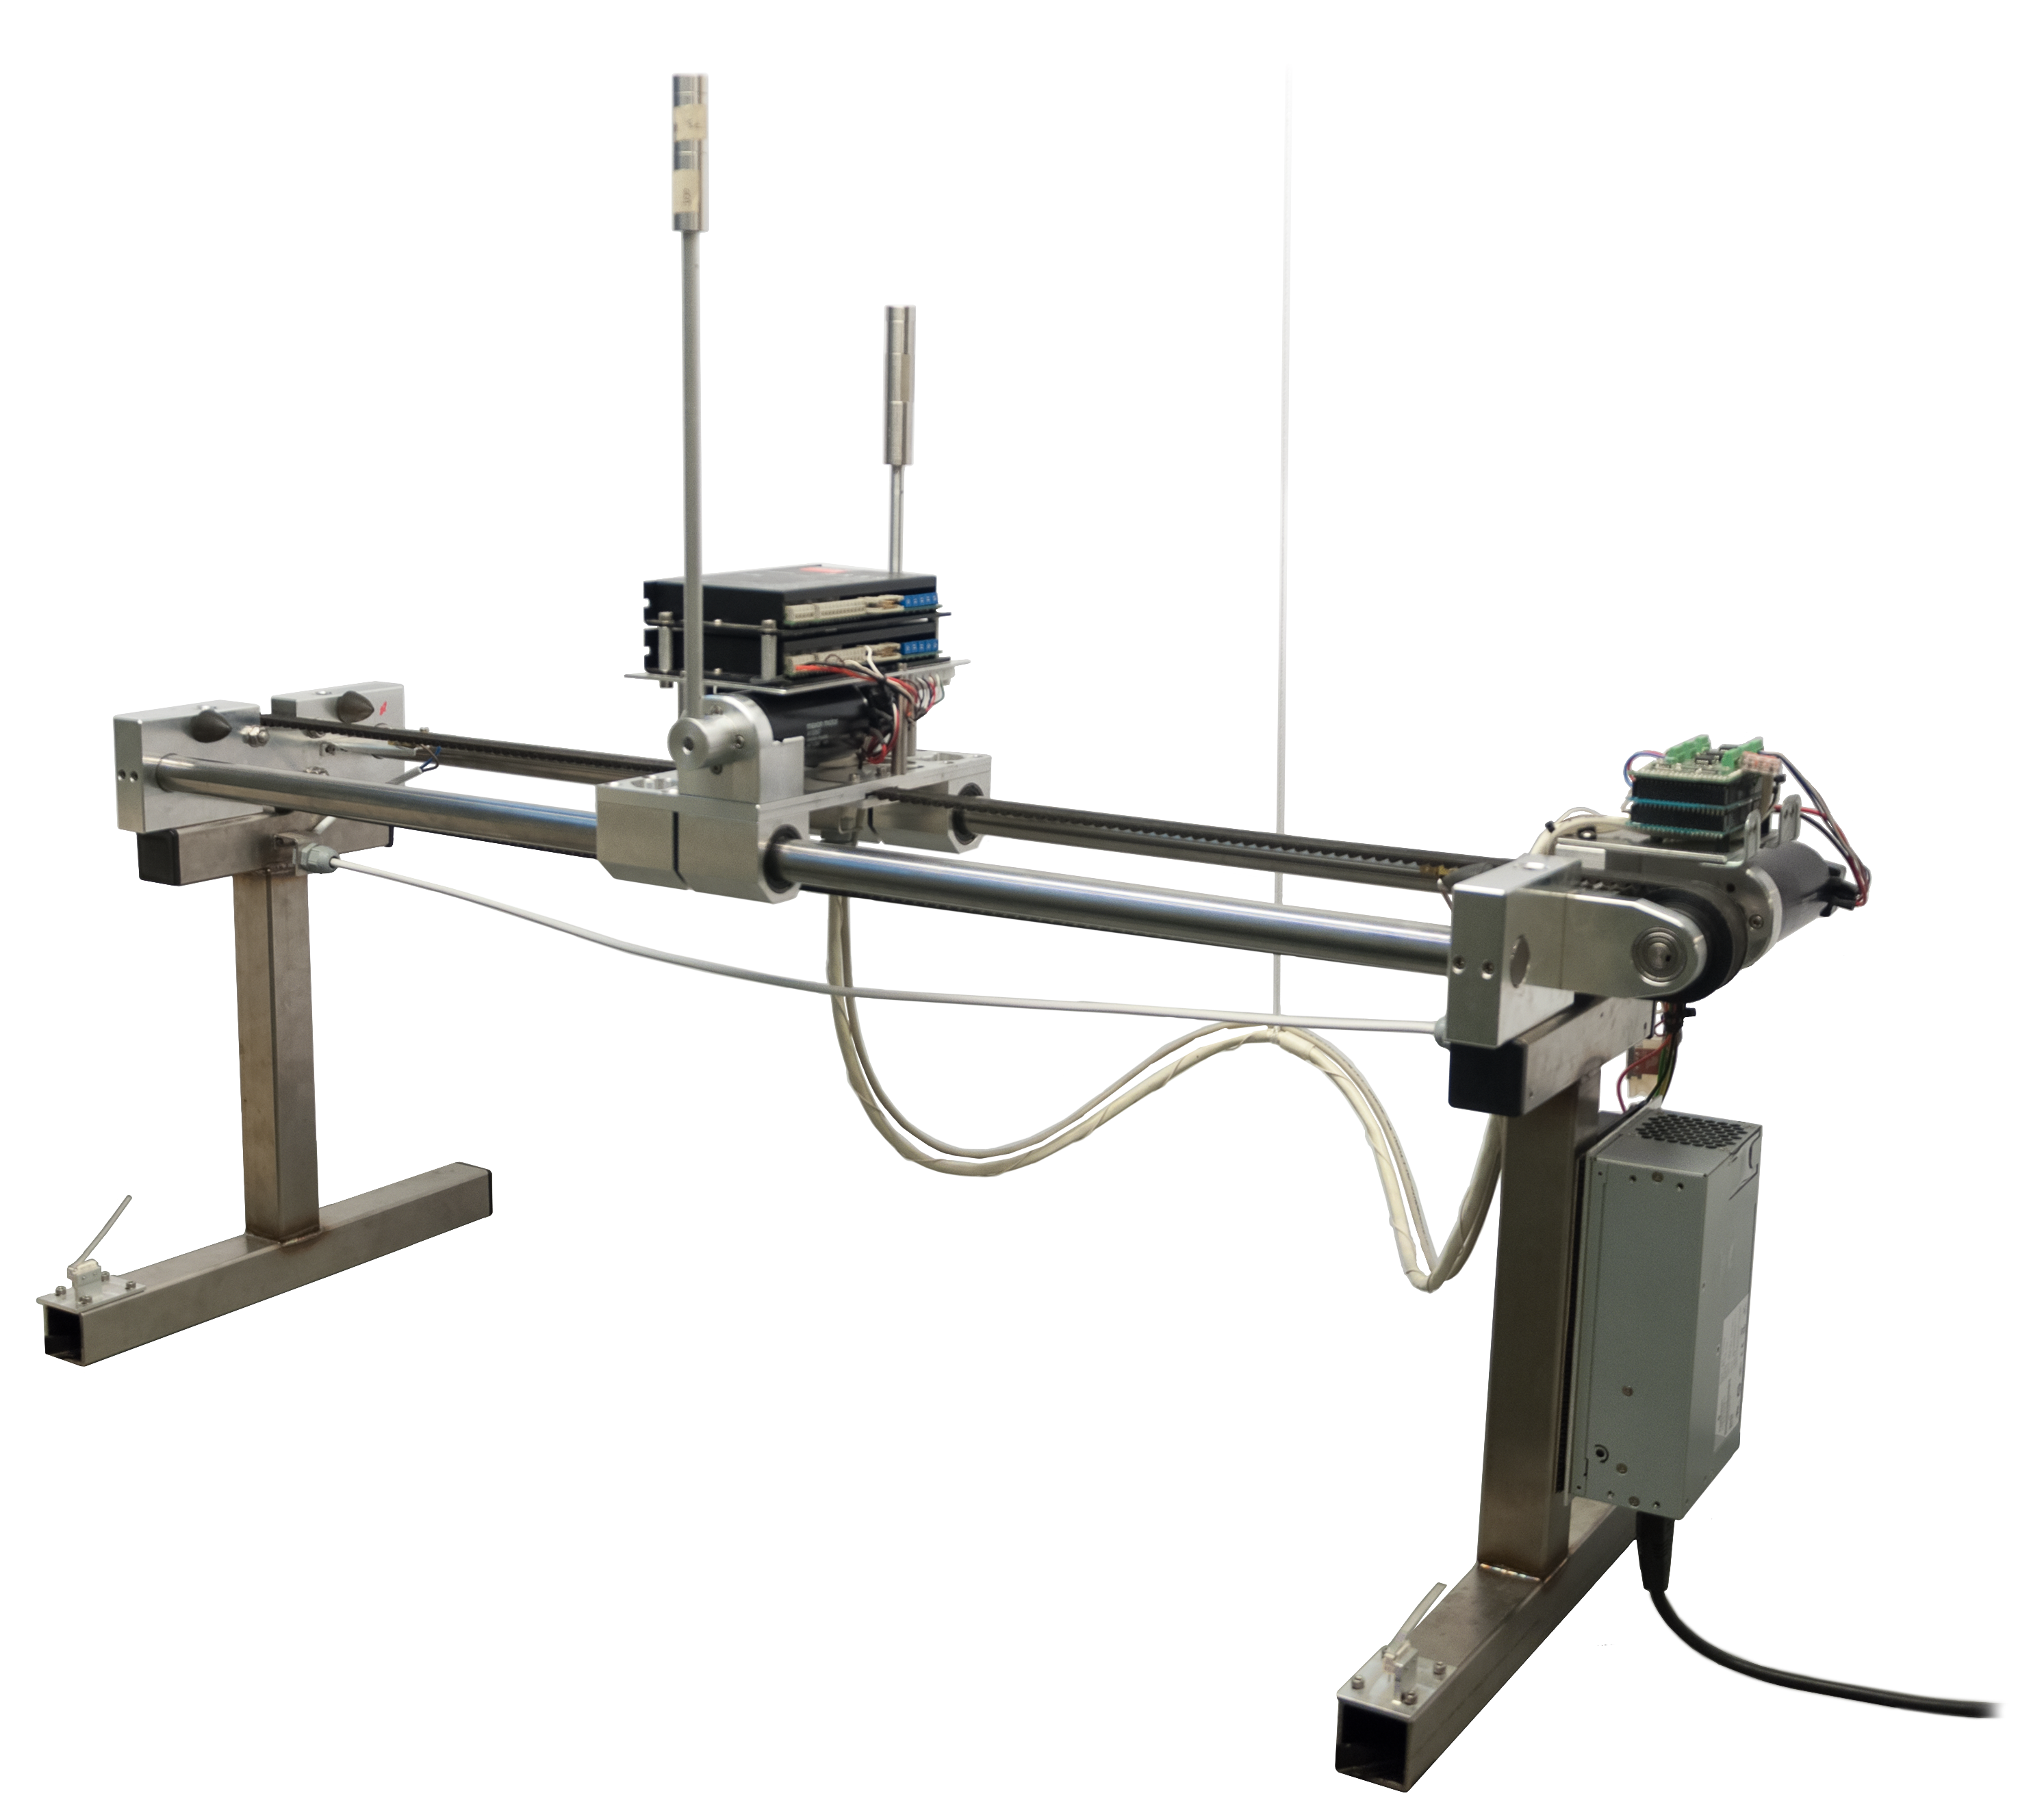
\includegraphics[width=\textwidth]{twinSetup}
  \end{center}
%  \begin{center}
%    \noindent\rule{5cm}{1pt}
%  \end{center}
  \vfill
  \begin{center}
    \textbf{by}
    
    \textbf{Niels Skov Vestergaard}
  \end{center}
\clearpage
\pagestyle{fancy}
%{\small
%\strut\vfill % push the content to the bottom of the page
%\noindent Copyright \copyright{} Aalborg University 2015\par
%\vspace{0.2cm}

%\noindent This report is compiled in \LaTeX, originally developed by Leslie Lamport, based on Donald Knuth's \TeX. The main text is written in \emph{Latin Modern} pt 12, designed by Bogusław Jackowski and Janusz M. Nowacki. 
%The document is compiled via the website \url{www.overleaf.com}, an online collaborative based \LaTeX-editor with instant preview, which enables multiple persons to edit the document simultaneously.
%Flowcharts and diagrams are made using Microsoft Visio. 
\clearpage
%\begin{document} 
%\thispagestyle{empty}
%\begin{titlepage}
\begin{nopagebreak}
{\samepage 

\begin{tabular}{r}
\parbox{\textwidth}{  \vspace{-1cm}\raisebox{-13mm}{
\includegraphics[height=3cm]{figures/aaulogo-en.png}}
\hfill \hspace{2cm} \parbox{8cm}{\begin{tabular}{l} %4.90
{\small \textbf{\textcolor{aaublue}{\colorbox{white}{Master Thesis}}}}\\
{\small \textbf{\textcolor{aaublue}{Control and Automation}}}\\ 
{\small \textcolor{aaublue}{Department of Electronic Systems}}\\
{\small \textcolor{aaublue}{Fredrik Bajers Vej 7C}}\\
{\small \textcolor{aaublue}{9220 Aalborg}} \vspace{1.2cm}\\
 \\
%{\small \textcolor{black}{\emph{http://www.sict.aau.dk/electronics-and-it}}}
\vspace{-2.5cm}
\end{tabular}}}
\end{tabular}

\begin{tabular}{cc}
\parbox{7cm}{

\textbf{Title:} \\
Swing-Up and Stabilization of a Cart Pendulum System and  Stabilization of a Twin Pendulum System \\

\textbf{Subtitle:} \\
Using Nonlinear Control Strategies \\

\textbf{Theme:} \\
\small{Nonlinear Control
\\
}

\parbox{8cm}{

\textbf{Project Period:}\\
Autumn 2018\\
%01/09/2016 - 20/12/2016\\
   
%\textbf{Project Group:}\\
%832\\ %\fxnote{Input group number}
  
\textbf{Participants:}\\
Niels Skov Vestergaard\\

\textbf{Supervisor:}\\John-Josef Leth\\
}

\textbf{Pages:} ? \\ 
\textbf{Appendices:} ? \\
\textbf{Attachments:} ? \\

\textbf{Concluded:} 2019-01-16\\

\vfill } &
\parbox{7cm}{
  \vspace{.15cm}
  \hfill
  \begin{tabular}{l}
  {\textbf{Synopsis:}} \\
  \fbox{
    \parbox{6.5cm}{\bigskip
     {\vfill{\small The aim of the project was to develop a sliding mode controller to stabilize a cart pendulum in its unstable equilibrium. Further to investigate a method for trajectory planning for a cart pendulum without friction. To find an interesting trajectory, a task was posed for the system to complete.\\
The system was modeled using both Newton's method and the energy method. The system was simulated using both simulink and matlab's ode45-solver. To aid in the process and to be able to visually show the results an animation was added to the simulations.\\
A sliding mode controller stabilizing the pendulum within $0.05$\fxnote{check value of real stability angle} rad was designed and implemented successfully. The posed task for trajectory planning was solved with a minor exception of bringing the pendulum to a compete stop at the end.
     \bigskip}}
     }}
   \end{tabular}}
\end{tabular} %\vspace{1cm}
}
\vspace{.5cm}

\textit{\phantom{A}Publication of this report's contents (including citation) without permission\\ \phantom{A}from the authors is prohibited}\\

\end{nopagebreak}
%\end{titlepage}
%\end{document}
%%% Preface %%%
%\cleardoublepage
%%%%%%%%%%%%%%%%%%%%%%%%%%%%%%%%%%%%%%%%%%%%%%%%5\chapter*{Preface}
\vspace{-12 pt}
\lipsum[3]\fxnote{Write prephase}

\textbf{Reading Instructions}
\vspace{-10 pt}
\begin{itemize}
\item[-] \lipsum[6]\fxnote{Write reading instructions}
\end{itemize}

%
\textbf{Text by:}\\
\vspace{-12 pt}
\begin{table}[H]
	\centering
		\begin{tabular}{c c c}
			&&\\
	    \multicolumn{3}{c}{\underline{\phantom{- Niels Skov Vestergaard -}}}\\
	    \multicolumn{3}{c}{Niels Skov Vestergaard}\\				
		\end{tabular}
\end{table}
\pagebreak

\pdfbookmark[0]{Table of Contents}{label: tableOfCentents}
\tableofcontents
\cleardoublepage


%%% Mainmatter Settings %%%
\pagenumbering{arabic} %use arabic page numbering in the mainmatter
\fancyfoot[RO,LE]{\thepage \text{ of} \pageref{LastPage}}
\fancyfoot[RE,LO]{}
\fancyhead[RE,LO]{}
\fancyhead[RE,LO]{\color{aaublue}\small\nouppercase\leftmark} %even page - chapter title
\pagestyle{fancy}

%---------- Chapter 1 ---------------------------------------- Introduction
\chapter{Introduction}
Two parts - two different systems and control objectives.

%%% PART 1 %%%
\part{Cart Pendulum}

%---------- Chapter 2 ---------------------------------------- System and Model
\chapter{System and Model}\label{chap:model}
A brief overview of the relevant system for \textit{Part 1} is presented in this chapter along with a model of the system.

\section{System}\label{sec:system}
A setup is provided by the Control and Automation Department at AAU, see \autoref{fig:systemSetup}.

\begin{figure}[H]
  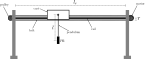
\includegraphics[width=\textwidth]{systemSetup}
  \caption{The setup provided by AAU. The motor controller in use is not directly visible in this picture as it is mounted behind the power supply.}
  \label{fig:systemSetup}
\end{figure}

As seen in \autoref{fig:systemSetup} the belt is attracted by pulleys one of which is driven by a brushed Maxon 370356 DC motor \cite{maxonMotor}. An other of these maxon motors is mounted on the pendulum but is disconnected and just used as a bearing in this project. Both motors are fitted with an HEDS 5540 optical quadrature encoder allowing for relative position and angle of the cart and pendulum respectively \cite{avagoTechnologies}.

The motor driving the belt is controlled using a Maxon ADS 50/10 motor controller configured in current control mode. The motor controller takes a $\pm$\SI{10}{V} input signal which then determines the armature current, $i_a$, see \cite{maxonMotorController}.

The primary control unit is a Teensy 3.6 microcontroller board. To program the board through the onboard USB connection a bootloader is used along with the Teensyduino add-on for the Arduino IDE \cite{sprkfunTeensy}.

The encoders are decoded on a shield using Avago HCTL-2021-PLC decoders and read through an 8 bit parallel data bus on the microcontroller board resulting in 2000 tics pr. revolution. This ensures a resolution for the pendulum angle, $\theta$, of $2\pi/2000=$ \SI{\pi e-3} rad/tic and $2\pi r /2000=\nolinebreak 2\pi\cdot 0.028 /2000\approx$ \SI{0.088e-3} m/tic for the cart position, $x$, see \cite{avagoDataSheet}.

The supply circuit on the microcontroller board is powered by 5V which is regulated to \SI{3.3}{V} resulting in a $0-$\SI{3.3}{V} range for the 12 bit analog output \cite{teensyDataSheet}. This output is used to provide the motor controller with an armature current reference, thus, the microcontroller analog output is amplified through the shield to meet the $\pm$\SI{10}{V} input requirement of the motor controller \cite{JHHorgensen}.

The following relation between analog 12 bit output values, $\text{bit}_\text{DAC}$, from the microcontroller and armature current in the motor was found by a previous project group \cite{JHHorgensen}, %linear regression
%
\begin{align}
  \text{bit}_\text{DAC} &= 105.78 \cdot i_{a} + 1970  \ \ \ , 
  \label{eq:Ia-bit}
\end{align}
%
and as a result of a force test, see \cite{NSVestergaard}, \autoref{eq:Ia-bit} was corrected to,
\begin{align}
  \text{bit}_\text{DAC} &= 111.9 \cdot i_{a} + 1970  \ \ \ ,
  \label{eq:Ia-bit-corrected}
\end{align}
which is the relation used in this project.
All the system parameters used in the design are listed in \autoref{table:systemParameters}. It is assumed that all frictions in the system can be modeled as a combination of Coulomb and viscous frictions. Wires hanging from the cart are unmodeled and their weight along with that of the belt are contained in the estimation of the cart mass. 

\begin{table}[H]
  \begin{tabular}{|l|l|l|l|}
    \hline %-----------------------------------------------------------------------------------------
    \textbf{Parameter}        & \textbf{Notation} & \textbf{Quantity} & \textbf{Unit}              \\
    \hline %-----------------------------------------------------------------------------------------
    Nominal current
    (max. continuous current) & $I_{\mathrm{N}}$  & \SI{4.58}         &  \si{A}                    \\
    \hline %-----------------------------------------------------------------------------------------
    Torque constant           & $\tau_m$          & \SI{93.4e-3}      &  \si{N\cdot m\cdot A^{-1}} \\
    \hline %-----------------------------------------------------------------------------------------
    Pendulum Rod Length       & $l$               & \num{0.3169}      &  \si{m}                    \\
    \hline %-----------------------------------------------------------------------------------------
    Rail Length               & $l_r$             & \num{0.89}        &  \si{m}                    \\
    \hline %-----------------------------------------------------------------------------------------
    Pulley Radius             & $r$               & \num{0.028}       &  \si{m}                    \\
    \hline %-----------------------------------------------------------------------------------------
    Pendulum Mass             & $m$               & \num{0.2235}      &  \si{kg}                   \\
    \hline %-----------------------------------------------------------------------------------------
    Cart Mass                 & $M$               & \num{6.28}        &  \si{kg}                   \\
    \hline %-----------------------------------------------------------------------------------------
    Cart Coulomb Friction     & $b_{c,c}$         & $f(x,\dot{x})$    &  \si{N}                    \\
    \hline %-----------------------------------------------------------------------------------------
    Cart Viscous Friction     & $b_{c,v}$         & \num{0}           &  \si{N\cdot m^{-1}\ s}      \\
    \hline %-----------------------------------------------------------------------------------------
    Pendulum Coulomb Friction & $b_{p,c}$         & \SI{4.1e-3}       &  \si{N\cdot m}             \\
    \hline %-----------------------------------------------------------------------------------------
    Pendulum Viscous Friction & $b_{p,v}$         & \SI{0.5e-3}       &  \si{N\cdot m\cdot s}      \\
    \hline %-----------------------------------------------------------------------------------------
  \end{tabular}
  \caption{The motor parameters, $I_{\mathrm{N}}$ and $\tau_m$, are given by maxon in \cite{maxonMotor}. The rod length is measured from the pendulum pivot point to the geometrical center of the pendulum mass. Pulley radius, rail length, pendulum mass and rod length, are measured parameters, while cart mass is estimated same as all frictions. The cart Coulomb friction turns out to be a function of the cart position in addition to velocity. Details on parameter estimation are found in the implementation section at the end of \textit{Part 1}.\label{table:systemParameters} }
\end{table}
%The estimations are performed by a previous project group \cite{JHHorgensen}.

\section{Model}\label{sec:model}
The model is based on the generalized coordinates presented in \autoref{fig:mechanicalDrawing}.
\begin{figure}[H]
  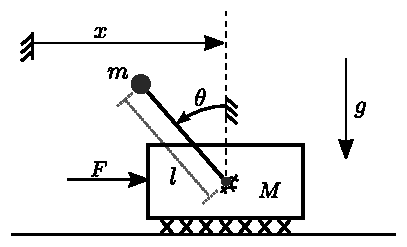
\includegraphics[width=.35\textwidth]{figures/mechanicalDrawing}
  \caption{Mechanical drawing of the system, where $\theta$ is the angle of the pendulum, $x$ is the position of the center of the cart along the rail, $F$ is the applied force and $g$ is the gravitational acceleration. It is indicated that friction is modeled between cart and rail as well as in the pendulum joint.}
  \label{fig:mechanicalDrawing}
\end{figure}
The pendulum mass center is positioned at zero hight at rest s.t. all energies in the system are positive. It is assumed that the pendulum rod is rigid and massless and that the pendulum weights are a point mass at the geometrical center of the weights.\\
The motor torque is given by direct relation to the armature current by the motor constant, $\tau_m = k_\tau i_a $, such that,
\begin{align}
  F &= \tfrac{1}{r} k_\tau i_a  \ \ \ .
\label{eq:motorForce}
\end{align}
%
To avoid excessive notation $u=F$ is considered to be the control input in the remaining of this thesis, while keeping in mind the relation in \autoref{eq:motorForce} along with the knowledge that $u$ must be converted to armature current in implementation.

%\begin{align}
%&& F &= \tfrac{1}{r} k_\tau i_a  &a
%\label{eq:motorForce}
%\end{align}
%
It is well known that the potential energy, $U$, and the kinetic energy, $T$, are given by, \cite{RWisniewski}
\begin{align}
  U &= mgl( 1 + \cos \theta )   \\
  T &= \frac{1}{2} ( M + m ) \dot{x}^2 - m \dot{x} l \cos \theta \dot{\theta} + \frac{1}{2} m l^2 \dot{\theta}^2 \ \ \ .
  \label{eq:generalizedPotentialAndKinetic}
\end{align}
The frictions, indicated in \autoref{fig:mechanicalDrawing}, are, as mentioned, comprised of Coulomb and viscous frictions with values stated in \autoref{table:systemParameters}. The viscous frictions are modeled as linear functions of velocities, \cite{CMClose, HOlsson}
\begin{align}
  b_{p,v} \dot{\theta} \ \ \ , & \ \ \ \ \ b_{c,v} \dot{x} \ \ \ , 
\label{eq:viscousFrictions}
\end{align}
for the rotational and linear case respectively.
The coulomb frictions are modeled as a constant with its sign depending on the signs of the velocities, such that, \cite{CMClose, HOlsson}
\begin{align}
  \mathrm{sgn}(\dot{\theta}) b_{p,c} \ \ \ , & \ \ \ \ \  \mathrm{sgn}(\dot{x}) b_{c,c} \ \ \ .
\label{eq:coloumbFrictions}
\end{align}
This, however, introduces discontinuities at zero velocities. Thus, tanh-functions are used to obtain a continues approximation of the sign-functions,
\begin{align}
  \tanh(\text{k}_\text{tanh}\dot{\theta}) b_{p,c} \ \ \ , & \ \ \ \ \ b_{c,v} \dot{x} - \tanh(\text{k}_\text{tanh}\dot{x}) b_{c,c} \ \ \ ,
\label{eq:coloumbFrictionsTanh}
\end{align}
where $\text{k}_\text{tanh}=250$ to increase the steepness of the tanh-functions thereby obtaining a closer approximation of the sign-functions.
Finally, by use of the Lagrange-d’Alembert Principle, \cite{RWisniewski}
\begin{align}
  \frac{d}{dt}  \frac{\partial \cal{L}}{\partial \dot{\vec{q}}} - \frac{\partial \cal{L}}{\partial \vec{q}}  &=  \vec{Q} \ \ \ ,
  \label{eq:energyMethodWithExternalForces}
\end{align}
\begin{align}
  \vec{q} &= 
  \begin{bmatrix}
    \theta    \\
    x
  \end{bmatrix} \ \ \ , \ \ \ 
  \vec{Q} =
  \begin{bmatrix}
    -b_{p,v} \dot{\theta} - \tanh(\text{k}_\text{tanh}\dot{\theta}) b_{p,c}    \\
    \tfrac{1}{r} k_\tau i_a - b_{c,v} \dot{x} - \tanh(\text{k}_\text{tanh}\dot{x}) b_{c,c}
  \end{bmatrix} \ \ \ ,
  \label{eq:qAndQ}
\end{align}
and $\cal{L} = T-U$, the dynamics of the system are found,
\begin{align}
  m l^2 \ddot{\theta} - m l \cos \theta \ddot{x} - m g l \sin \theta  &= -b_{p,v} \dot{\theta} - \tanh(\text{k}_\text{tanh}\dot{\theta}) b_{p,c} \label{eq:energyDerivedDynamicEquation2} \\
  ( M + m )\ddot{x} + m l \sin \theta \dot{\theta}^2 - m l \cos \theta \ddot{\theta}  &=  u - b_{c,v} \dot{x} - \tanh(\text{k}_\text{tanh}\dot{x}) b_{c,c} \ \ \ .
  \label{eq:energyDerivedDynamicEquation1}
\end{align}
By setting up the dynamic equations, \autoref{eq:energyDerivedDynamicEquation1} and \ref{eq:energyDerivedDynamicEquation2}, in the following manner,
%
\begin{align}
\begin{split}
  &
  \begin{bmatrix}
    m l^2              & -m l \cos \theta  \\
    -m l \cos \theta   & M + m
  \end{bmatrix}
  \begin{bmatrix}
    \ddot{\theta}  \\
    \ddot{x}
  \end{bmatrix}
  +
  \begin{bmatrix}
    0  \\
    m l \sin \theta \dot{\theta}^2
  \end{bmatrix}
  +   \\
  &+
  \begin{bmatrix}
    b_{p,v} \dot{\theta} + \tanh(\text{k}_\text{tanh}\dot{\theta}) b_{p,c}    \\
    b_{c,v} \dot{x} + \tanh(\text{k}_\text{tanh}\dot{x}) b_{c,c}
  \end{bmatrix}
  +
  \begin{bmatrix}
    -m g l \sin \theta  \\
    0
  \end{bmatrix}
  =
  \begin{bmatrix}
    0  \\
    u
  \end{bmatrix} \ \ \ , 
\end{split}
\label{eq:thetaXdynamics}
\end{align}
%
the general form of an m-link robot is obtained, \cite{MWSpong, LSciavicco}
\begin{align}
  \vec{M}(\vec{q})\vec{\ddot{q}} + \vec{C}(\vec{q},\vec{\dot{q}}) + \vec{B}(\vec{\dot{q}}) + \vec{G}(\vec{q}) &= \vec{F} \ \ \ , \hspace{3.3cm}
\end{align}
\begin{where}
  \va{ \vec{M}(\vec{q})  }{is the inertia matrix}                    {}
  \va{ \vec{C}(\vec{q},\vec{\dot{q}})  }{is the Coriolis and centrifugal effects}  {}
  \va{ \vec{B}(\vec{\dot{q}})          }{is the friction}                          {}
  \va{  \vec{G}(\vec{q})               }{is the force due to gravity}              {}
  \va{  \vec{F}                        }{is the input force vector \ \ \ .}        {}
\end{where}

Choosing $ [\ x_1\ \ x_2\ \ x_3\ \ x_4\ ]^\mathrm{T} = [\ \theta\ \ x\ \ \dot{\theta}\ \ \dot{x}\ ]^\mathrm{T} $ as states results in the following nonlinear state space representation,
%
\begin{align}
  \begin{bmatrix}
    \dot{x_1} \\
    \dot{x_2} \\
    \dot{x_3} \\
    \dot{x_4}
  \end{bmatrix}
&=
  \left[
    \begin{array}{c}
      x_3 \\
      x_4 \\
      \multirow{2}{*}{$ \vec{M}^{-1}(x_1) ( \vec{F} - \vec{C}(x_1,x_3) - \vec{B}(x_3,x_4) - \vec{G}(x_1) ) $}\\
      \phantom{eq}
    \end{array}
  \right]
  \label{eq:nonlinearStateSpace} \ \ \ ,
\end{align}
%
which is convenient when simulating the system. This representation is also used in the controller designs.




%---------- Chapter 3 ---------------------------------------- Swing-Up
\chapter{Swing-Up Design}\label{sec:swing-upDesign}
In this chapter four swing-up controllers are designed, all based on \cite{kjAastrom}. The pendulum is started at rest, $\theta = \pi$, with the angle convention specified in \autoref{fig:mechanicalDrawing}. The idea of the swing-up controller is to increase the mechanical energy in the system until it matches that of the desired end state, $\theta = 0$ and $\dot{\theta} = 0$, that is, the upright position at rest. The minimum energy in the system occurs at the starting position at rest, which is considered to be zero as mentioned in the \textit{Model} \autoref{sec:model}. So the target energy is $E_{\mathrm{eq}} = 2 m g l$, that is, the potential energy of the pendulum in the unstable equilibrium.

Consider the pendulum dynamics from \autoref{eq:energyDerivedDynamicEquation1}, where $J = m l^2$ is the pendulum inertia and frictions are assumed to be zero such that,
\begin{flalign}
&& J \ddot{\theta} - m l \cos \theta a_c - m g l \sin \theta  &= 0 \ \ \ , &  \unit{N \cdot m}   \label{eq:pendulumDynamics}
\end{flalign}
This equation captures the behavior of the pendulum corresponding to some controlled acceleration $a_c$ at the pivot point. This acceleration is viewed as the control input for now. The force needed to achieve this acceleration is considered in the end of the design. It is further convenient to describe the energy of the pendulum with the coordinate frame fixed at its pivot point, see \autoref{fig:fixedCooredinateSystem}.
%
\begin{figure}[H]
  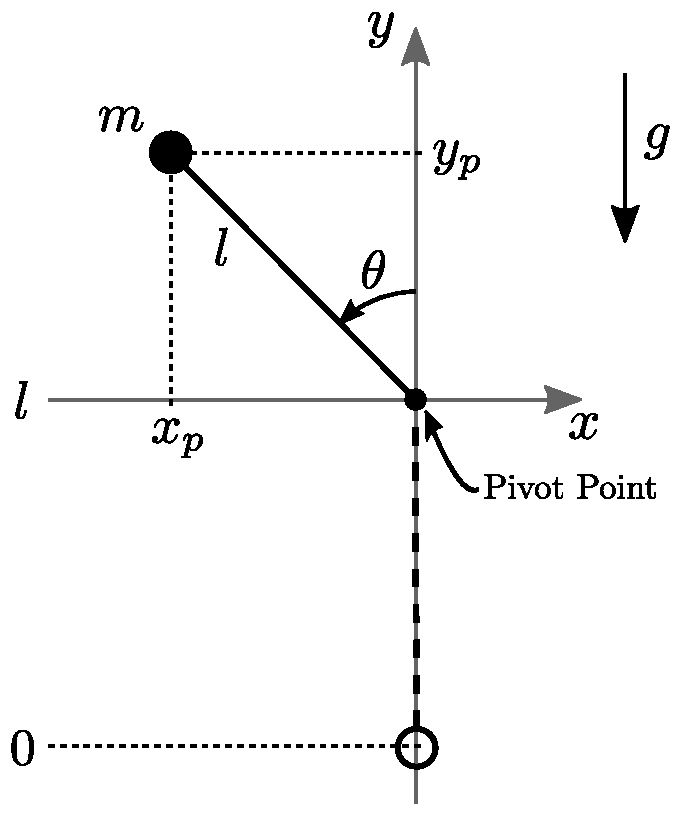
\includegraphics[width=.3\textwidth]{figures/fixedCooredinateSystem}
  \caption{The energy used in the swing-up controller is described using this convention, where the coordinate frame is fixed at the pivot point of the pendulum. The zero reference is placed as before s.t. all energies are positive.}
  \label{fig:fixedCooredinateSystem}
\end{figure}
%
From \autoref{fig:fixedCooredinateSystem}, the conversion from excessive to generalized coordinates is given by,
\begin{flalign}
&& x_p  &= -l \sin \theta   \ \ \ ,\ \ \ y_p = l(\cos \theta + 1)  \ \ \ ,\ \ \ \dot{x}_p = -l \cos \theta \dot{\theta}  \ \ \ ,\ \ \ \dot{y}_p = -l \sin \theta \dot{\theta}  \ \ \ . &&     \label{eq:cooredinateConvertFixed}
\end{flalign}
The mechanical energy in this coordinate frame is then,
\begin{flalign}
&& E_p &= m g y_p + \tfrac{1}{2} m \dot{x}_p^2 + \tfrac{1}{2} m \dot{y}_p^2  &  \unit{J}   \label{eq:pendulumEnergy1} \\
&& E_p &= m g l (\cos \theta +1) + \tfrac{1}{2} m (-l \cos \theta \dot{\theta})^2 + \tfrac{1}{2} m (-l \sin \theta \dot{\theta})^2  &  \unit{J}   \label{eq:pendulumEnergy2} \\
&& E_p &= m g l (\cos \theta +1) + \tfrac{1}{2} J (\cos^2 \theta  + \sin^2 \theta )\dot{\theta}^2  &  \unit{J}   \label{eq:pendulumEnergy3} \\
&& E_p &= \tfrac{1}{2} J \dot{\theta}^2 + m g l (\cos \theta +1) \ \ \ . &  \unit{J}   \label{eq:pendulumEnergy4}
\end{flalign}
The following sections explores different approaches of controlling the pendulum energy specified in \autoref{eq:pendulumEnergy4} to its desired reference.

\subsection{Energy Control}
A Lyapunov function candidate is proposed,
\begin{flalign}
&& V &= \tfrac{1}{2} E_\Delta ^2 \ \ \ ,  \hspace{5cm}  &&&  \label{eq:lyapunovCandidate} 
\end{flalign}
where $E_\Delta$ is the difference in energy in relation to the unstable equilibrium,
%
\begin{flalign}
&& E_\Delta &= E_p  - E_{\mathrm{eq}} &  \unit{J}   \label{eq:energyDelta1} \\
&& E_\Delta &= \tfrac{1}{2} J \dot{\theta}^2 + m g l (\cos \theta +1) - 2 m g l &  \unit{J}   \label{eq:energyDelta2} \\
&& E_\Delta &= \tfrac{1}{2} J \dot{\theta}^2 + m g l (\cos \theta -1)   \ \ \ .  & \unit{J} \label{eq:energyDelta3}
\end{flalign}
%
The idea is to reach the reference $E_\Delta = 0$, which happens when,
\begin{flalign}
  &&& \tfrac{1}{2} J \dot{\theta}^2 + m g l (\cos \theta -1) = 0 && \label{eq:energyDeltaZero1} \\
  &&& \dot{\theta} = \pm \left(\frac{-2 m g l (\cos \theta -1)}{J}\right)^{\tfrac{1}{2}}  \ \ \ .  && \label{eq:energyDeltaZero2}
\end{flalign}
%
A plot of \autoref{eq:energyDeltaZero2} in the phase plane, see \autoref{fig:orbit}, reveals a set of solutions joining the two unstable equilibrium points.
%
\begin{figure}[H]
  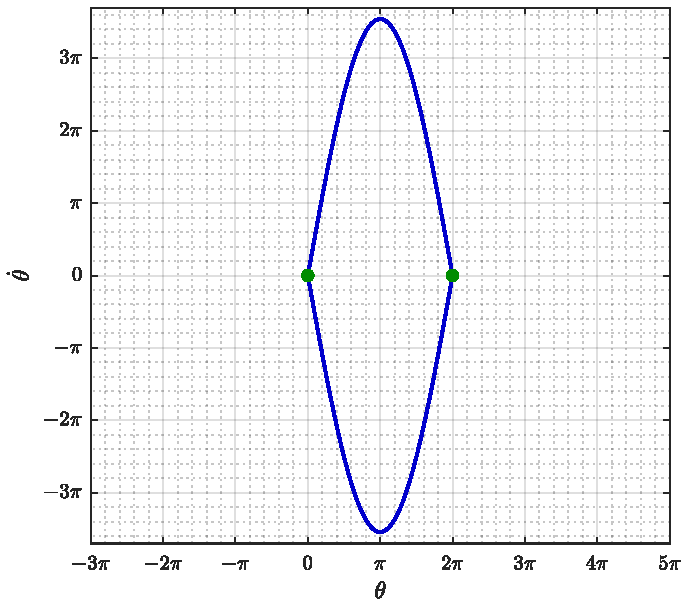
\includegraphics[width=.4\textwidth]{figures/orbit}
  \caption{orbit}
  \label{fig:orbit}
\end{figure}
%
If the energy reference is successfully tracked, the system will be restricted to this set rather than a single equilibrium point. Such a trajectory joining two equilibrium points is called a heteroclinic orbit.\\
Following \autoref{th:lyapunovStabilityTheorem}, the derivative of the Lyapunov function candidate, \autoref{eq:lyapunovCandidate},
\begin{flalign}
&& \dot{V} &= E_\Delta \dot{E}_\Delta  \ \ \ ,\ \ \ \ \dot{E}_\Delta = J \dot{\theta} \ddot{\theta} - m g l \sin \theta \dot{\theta}  \ \ \ , \hspace{3cm}  &&&  \label{eq:lyapunovDerivative1}
\end{flalign}
is $C^0$ and thus $V(x)$ is continuously differentiable, $C^1$. Further, $V(\vec{0}) = 0$ and $V(\vec{x})>0$ in the entire state space, excluding zero.
%The Lyapunov function candidate, \autoref{eq:lyapunovCandidate}, is continuously differentiable in the entire $\mathbb{R} ^2$. Its derivative is evaluated to find a stabilizing controller,
%
\begin{theorem}[Lyapunov Stability Theorem]
  \label{th:lyapunovStabilityTheorem}
  Consider the autonomous system, $f(\vec{x}) = \dot{\vec{x}}$, where $f : \mathbb{D} \rightarrow \mathbb{R} ^n$ is locally Lipschitz and $\vec{x}=\vec{0}$ is an equilibrium point. Then if $\exists\ V : \mathbb{D} \rightarrow \mathbb{R}$ and \vspace{-12pt}
  \begin{enumerate}
    \item $V(\vec{x})$ is $C^1$
    \item $V(\vec{x}) > 0$ $\forall x \in \mathbb{D}\backslash 0$ and $V(\vec{0}) = 0$
    \item $\dot{V}(\vec{x}) \leq 0$ in $\mathbb{D}$
  \end{enumerate} \vspace{-12pt}
  then $\vec{x} = \vec{0}$ is stable. Further, if,
  \begin{flalign}
    && \dot{V}(\vec{x}) &< 0\ \mathrm{in}\ \mathbb{D}\backslash 0  \ \ \ ,  \hspace{3cm}  &&&  \nonumber
  \end{flalign}
  then $\vec{x} = \vec{0}$ is asymptotically stable \cite{HKKhalil}.
\end{theorem}\vspace{-12pt}
%
The third condition states that the derivative of the Lyapunov function candidate along trajectories of the system must be less than or equal to zero in the entire state space. In this case, from \autoref{eq:lyapunovDerivative1}, if the energy error goes to zero, so does the derivative of the Lyapunov function.\\
Without checking for definiteness, it is known that in cases where $V(\vec{x}) = 0$, trajectories neither approach nor diverge from the equilibrium, but rather stay in some orbit. While \autoref{th:lyapunovStabilityTheorem} has the potential to promise stability of the desired orbit once there, it does not guarantee convergence to said orbit.\\
However, by instead studying LaSalle's \autoref{th:lasallesTheorem}, analysis of convergence to sets is made possible.
\begin{theorem}[LaSalle's Theorem]
  \label{th:lasallesTheorem}
  Consider again the system from \autoref{th:lyapunovStabilityTheorem}. Then if there exist some function $V : \mathbb{D} \rightarrow \mathbb{R}$ and \vspace{-12pt}
  \begin{enumerate}
    \item $V(\vec{x})$ is $C^1$
    \item $\exists\ c > 0$ s.t. $\Omega_c = \{\vec{x} \in \mathbb{R}^n \ | \ V(\vec{x}) \leq c \} \subset \mathbb{D}$ is bounded
    \item $\dot{V}(\vec{x}) \leq 0 \ \ \forall \ \vec{x} \in \Omega_c$
  \end{enumerate} \vspace{-12pt}
  then $\vec{x}(0) \in \Omega_c \Rightarrow \vec{x}(t) \xrightarrow[]{t \to \infty} M \ ,$  where $M$ is the largest invariant set in\vspace{-12pt}
  \begin{itemize}
    \item[] $E = \{ \vec{x} \in \Omega_c \ | \ \dot{V}(\vec{x}) = 0 \} \ \ $ \cite{HKKhalil}.
  \end{itemize}\vspace{-12pt}
\end{theorem}
%
Though the function $V(\vec{x})$ is not required to be positive definite by \autoref{th:lasallesTheorem}, the same function candidate, \autoref{eq:lyapunovCandidate}, is used, thereby satisfying the first condition.\\
The second condition states that some bounded set, $\Omega_c$, of solutions for which $V(x)$ is less than or equal to some constant $c$ must exist.\\
This ties into the third condition stating that the derivative of the function candidate must be negative semi-definite along trajectories of the system for all solutions in said set.\\
To find $\Omega_c$, the derivative of the function candidate,  \autoref{eq:lyapunovDerivative1}, is evaluated along the trajectories of the system, \autoref{eq:pendulumDynamics},
\begin{flalign}
&& \dot{V} &= E_\Delta ( J \dot{\theta} \ddot{\theta} - m g l \sin \theta \dot{\theta} ) \hspace{3cm}  &&&  \label{eq:lyapunovDerivative2} \\
&& \dot{V} &= E_\Delta ( \dot{\theta} ( m l \cos \theta a_c + m g l \sin \theta )  - m g l \sin \theta \dot{\theta} )  &&&  \label{eq:lyapunovDerivative3} \\
&& \dot{V} &= m l E_\Delta \cos \theta \dot{\theta} a_c   \ \ \ ,  \label{eq:lyapunovDerivative4}
\end{flalign}
%
The controlled acceleration at the pivot point, $a_c$, is then designed to satisfy the third condition in \autoref{th:lasallesTheorem},
\begin{flalign}
&& \dot{V} &= m l E_\Delta \cos \theta \dot{\theta} (-k E_\Delta \cos \theta \dot{\theta})     \hspace{2cm}  &&&  \label{eq:lyapunovDerivativeControlled1} \\
&& \dot{V} &= -k m l (E_\Delta \cos \theta \dot{\theta})^2  \leq 0  \ \ \ ,  \hspace{2cm}  &&&  \label{eq:lyapunovDerivativeControlled2} 
\end{flalign}
the tuning parameter, $k>0$, is introduced to allow scaling the control output to fit the capabilities of the actuator. The control law for the acceleration of the pivot point is,
\begin{flalign}
&& a_c &= -k E_\Delta \cos \theta \dot{\theta}  \ \ \ .  \hspace{4cm}  &&&  \label{eq:accControlLaw}
\end{flalign}
This control law satisfies the third condition of \autoref{th:lasallesTheorem} not only in $\Omega_c$ but in the entire state space. This means any $c>0$ will satisfy the second condition. It also satisfies the first stability criterion of \autoref{th:lyapunovStabilityTheorem}, indicating the control law has caused stability of equilibrium. However, the equilibrium points are not the only stable points using this control strategy, and, as stated, \autoref{th:lyapunovStabilityTheorem} does not guarantee convergence to a set.\\
All conditions of LaSalle's \autoref{th:lasallesTheorem} are satisfied, thus, if starting in $\Omega_c$, trajectories of the system will converge to $M$ as time goes to infinity. As this set, $M$, is the largest invariant set in $E$, which can be described as the union of sets for which \autoref{eq:lyapunovDerivativeControlled2} is zero,
\begin{flalign}
&& E  &= \{ \vec{x} \in \Omega_c \ | \ E_\Delta = 0 \} \cup  \{ \vec{x} \in \Omega_c \ | \  \cos \theta = 0 \} \cup  \{ \vec{x} \in \Omega_c \ | \ \dot{\theta} = 0 \} \ \ \ .   &&&  \label{eq:E}
\end{flalign}
\fxnote{Kan man skrive sæt på den måde? Er der en bedre måde?}
\fxnote{Hvordan ved jeg at E Delta er invariant?}
The only way $\cos \theta = 0$ is part of an invariant set, is in situations where it is contained in the set for which $E_\Delta = 0$, any other values of the angular velocity will cause it to leave the set. The same argument is used for $\dot{\theta} = 0$, however, in this case if $\theta = \pm \pi n , \ n = 1, 3, 5, ...$, the system stays. So the largest invariant set in $E$ is,
\begin{flalign}
&& M  &= \{ \vec{x} \in \Omega_c \ | \ E_\Delta = 0 \} \cup  \{ \vec{x} \in \Omega_c \ | \ \dot{\theta} = 0 \ | \ \theta = \pm \pi n , \ n = 1, 3, 5, ... \} \ \ \ .    &&&  \label{eq:M}
\end{flalign}
%
If this control law is started at zero angular velocity, $\dot{\theta} = 0$, in a stable equilibrium, the computed control is maintained at zero and the pendulum never swings up. So for this control law to work, the pendulum must be started slightly away from a stable equilibrium.

An extra step is needed to apply this control strategy. So far the control output is an acceleration, $a_c$, at the pivot point. It is possible to input the desired acceleration, $a_c$, into the second dynamic equation, \autoref{eq:energyDerivedDynamicEquation1}, and solve for the force needed to achieve this acceleration,
%
\begin{flalign}
  && u &=  ( M + m )a_c + m l \sin x_1 x_3^2 - m l \cos x_1 \dot{x}_3  \ \ \ , &   \unit{N}
  \label{eq:forceDynamics}
\end{flalign}
%
where the cart friction coefficients are set to zero again.\\
To calculate the force from this expression, \autoref{eq:forceDynamics}, it is also necessary to know the angular acceleration of the pendulum, $\dot{x}_3$, which can be solved for in the system dynamics, \autoref{eq:nonlinearStateSpace}, inserting known states and control input applied in the previous step,
%
\begin{flalign}
  &&
    \begin{bmatrix}
      \dot{x}_3  \\
      \dot{x}_4
    \end{bmatrix}
    &=
    \begin{bmatrix}
      m l^2           & -m l \cos x_1  \\
      -m l \cos x_1   & M + m
    \end{bmatrix}^{-1}
    \begin{bmatrix}
      - b_{p,v} x_3 - \tanh(\text{k}_\text{tanh}x_3) b_{p,c} + m g l \sin x_1 \\
      u_{last} - m l \sin x_1 x_3^2
    \end{bmatrix}
     \ \ \ ,  &&
  \label{eq:nonlinearStateSpaceQdotDot}
\end{flalign}
%
where $u_{last}$ is the force applied in the previous step.\\
From \autoref{eq:nonlinearStateSpaceQdotDot} the approximated angular acceleration is then,
\begin{flalign}
  && \dot{x}_3 &= \frac{ ( M + m )(- b_{p,v} x_3 - \tanh(\text{k}_\text{tanh}x_3) b_{p,c} + m g l \sin x_1) }{ l^2 m ( M + m - m \cos^2x_1 ) }
                    + \frac{ \cos x_1 (u_{last} - m l \sin x_1 x_3^2) }{ l ( M + m - m \cos x_1^2 ) }
  \ \ \ .  &&
  \label{eq:thetaDotDotApprox}
\end{flalign}
%
Inserting \autoref{eq:thetaDotDotApprox} into \autoref{eq:forceDynamics} results in the control input, $u$, necessary to achieve the desired acceleration, $a_c$, at the pivot point. This method is used for all four swing-up controllers, so to avoid excessive notation the proceeding energy control laws are derived with $a_c$ as the control parameter.

All simulations are performed using the nonlinear state space representation in \autoref{eq:nonlinearStateSpace} and the matlab ODE45 solver with relative tolerance of \SI{1e-7}{}. Initializing the angle, $\theta$, at $\pi-0.1$ to avoid zero control output as discussed, the energy difference struggles to reach its reference at zero, see \autoref{fig:Edelta_1_noConX}. The pendulum friction and cart inertia are included in the calculation of the force needed to obtain the desired acceleration. This, however, is not concerned with what is needed to obtain the required energy. So the offset seen in \autoref{fig:Edelta_1_noConX} is caused by the control law, \autoref{eq:accControlLaw}, asking for insufficient acceleration.
%
\begin{figure}[H]
  \hspace{-10pt}
  \captionbox
  {
    Simulation of the first energy control method. The energy error struggles to maintain zero value, due to pendulum friction and cart inertia exchanging energy with the pendulum.
    \label{fig:Edelta_1_noConX}
  }
  {
    \hspace{-1cm}
    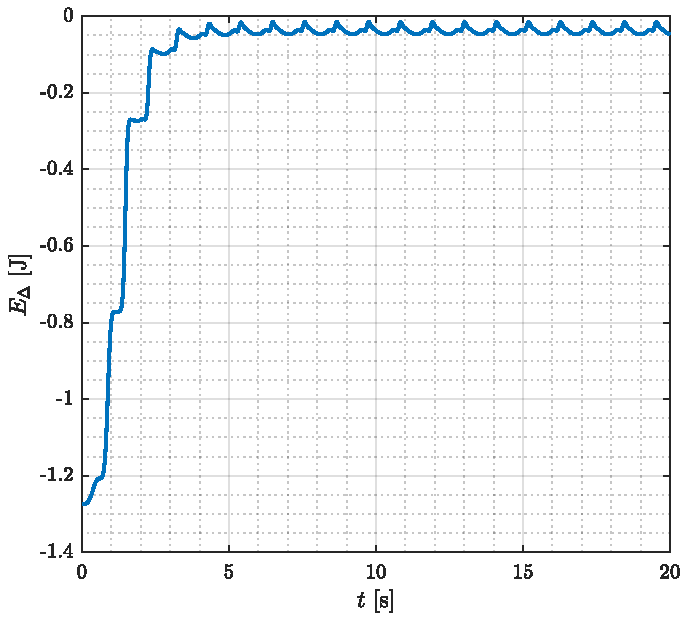
\includegraphics[width=.46\textwidth]{figures/Edelta_1_noConX}
  }
  \hspace{20pt}
  \captionbox 
  {
    This phase portrait shows the attempt to reach the heteroclinic orbit. It falls short due to the insufficient acceleration asked by the control law.
    \label{fig:phase_1_noConX}
  }
  {
    \hspace{-1cm}
    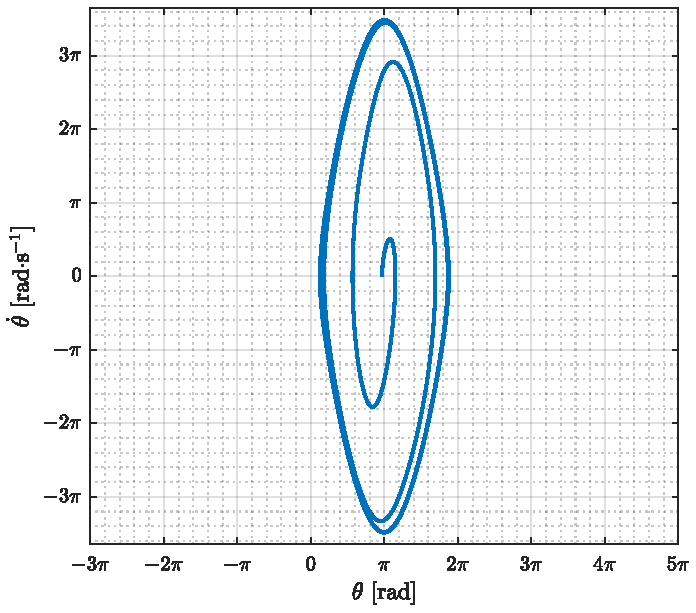
\includegraphics[width=.46\textwidth]{figures/phase_1_noConX}
  }  
\end{figure}
%
The pendulum also falls short of reaching the heteroclinic orbit, see \autoref{fig:phase_1_noConX}.
Further, since the energy of the pendulum is not affected by the position or velocity of the cart, this control law, \autoref{eq:accControlLaw}, is not concerned with controlling these. This becomes a problem in the physical setup as it has a rail length of \SI{0.89}{m}, see \autoref{table:systemParameters}. A traced animation is used to demonstrate this problem in \autoref{fig:ani_1_noConX}.
\begin{figure}[H]
  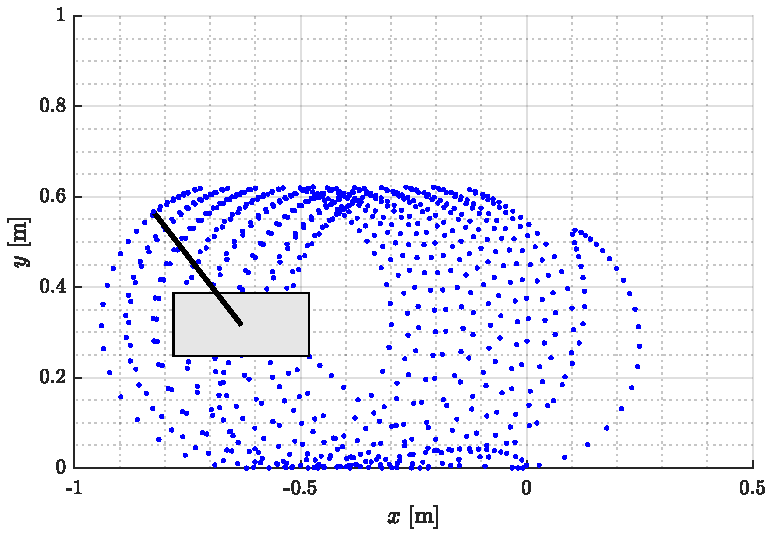
\includegraphics[width=.7\textwidth]{figures/ani_1_noConX}
  \caption{The cart drifts beyond the bounds of the physical system. This might not be a problem if the catch controller catches the pendulum in first try, but there is no guarantee of this being the case.}
  \label{fig:ani_1_noConX}
\end{figure}
%
An other issue is the actuation which is limited in the real system by the maximum allowed continuous current, see \autoref{table:systemParameters}. By tuning the parameter $k$ in \autoref{eq:accControlLaw}, better performance can be obtained, however at the cost of excessive actuation.
%
\begin{figure}[H]
  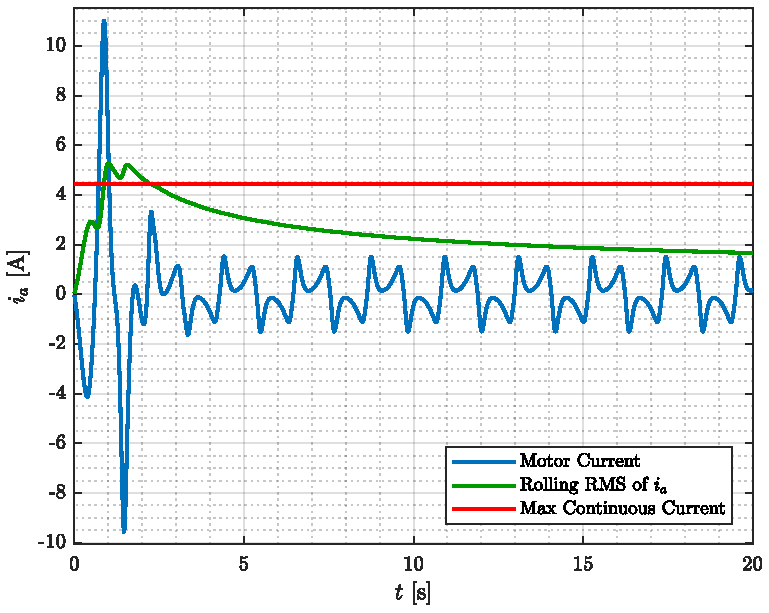
\includegraphics[width=.52\textwidth]{figures/ia_1_noConX}
  \caption{The motor current has high peaks in the beginning which likely exceeds the capabilities of the motor. The controller is tuned such that the RMS value of the current does not exceed the maximum continuous current requirement of the motor for a sustained period of time.}
  \label{fig:ia_1_noConX}
\end{figure}
%
For these graphs $k=1.3$ to keep the motor current at acceptable levels. The motor current is shown in \autoref{fig:ia_1_noConX} where the rolling RMS of $i_a$ is used to approximate the continuous current load on the motor.

%\begin{figure}[H]
%  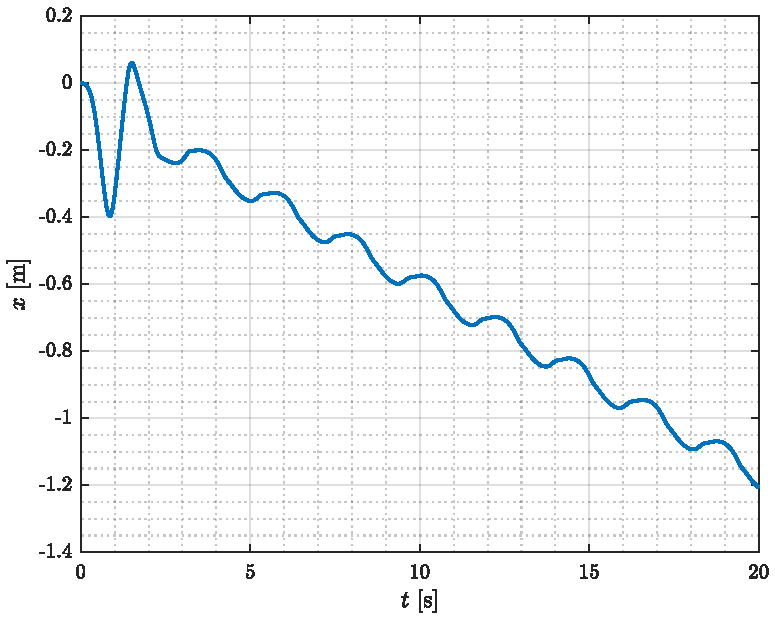
\includegraphics[width=.6\textwidth]{figures/x_1_noConX}
%  \caption{x1noConX}
%  \label{fig:x_1_noConX}
%\end{figure}
%\begin{figure}[H]
%  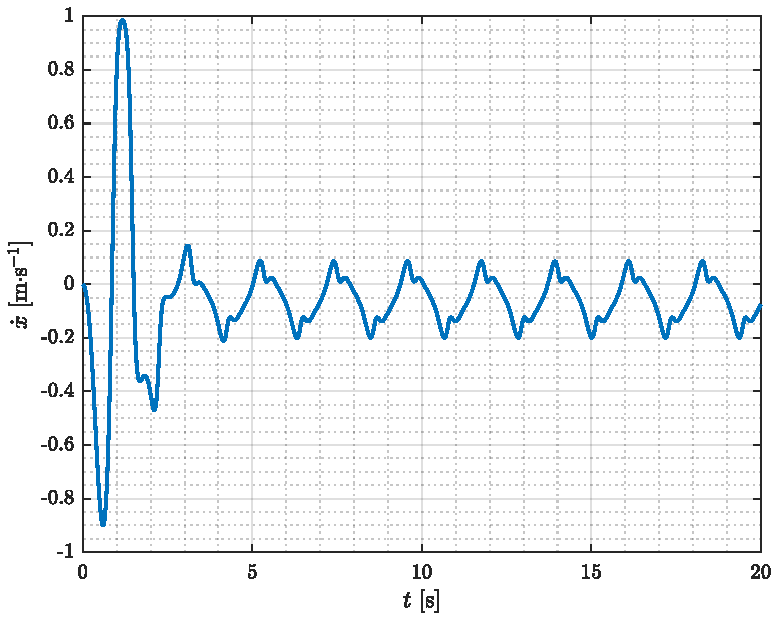
\includegraphics[width=.6\textwidth]{figures/xDot_1_noConX}
%  \caption{xDot1noConX}
%  \label{fig:xDot_1_noConX}
%\end{figure}
%\begin{figure}[H]
%  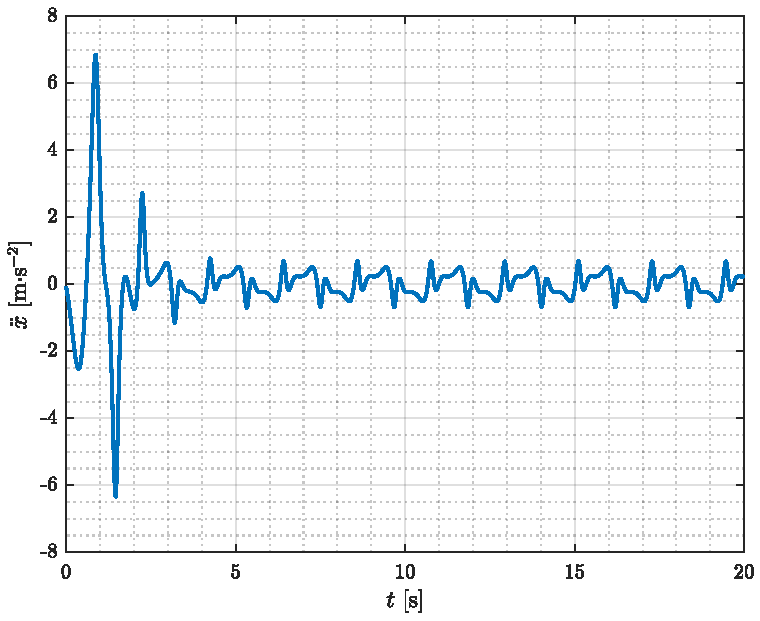
\includegraphics[width=.6\textwidth]{figures/xDotDot_1_noConX}
%  \caption{xDotDot1noConX}
%  \label{fig:xDotDot_1_noConX}
%\end{figure}
%\begin{figure}[H]
%  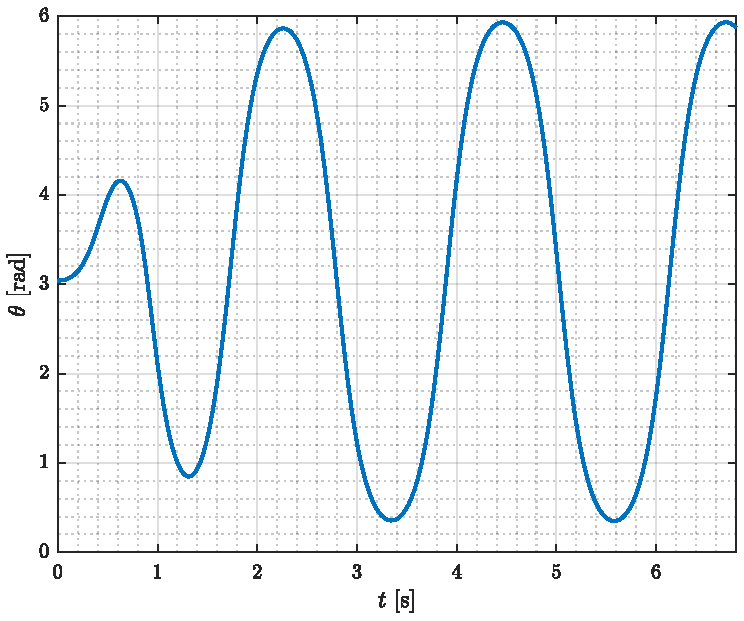
\includegraphics[width=.6\textwidth]{figures/theta_1_noConX}
%  \caption{theta1noConX}
%  \label{fig:theta_1_noConX}
%\end{figure}
%\begin{figure}[H]
%  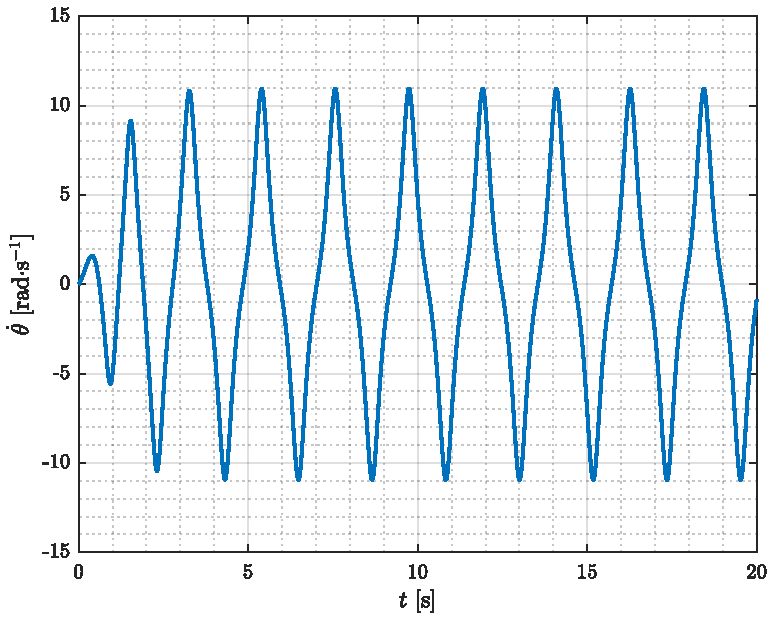
\includegraphics[width=.6\textwidth]{figures/thetaDot_1_noConX}
%  \caption{thetaDot1noConX}
%  \label{fig:thetaDot_1_noConX}
%\end{figure}
%\begin{figure}[H]
%  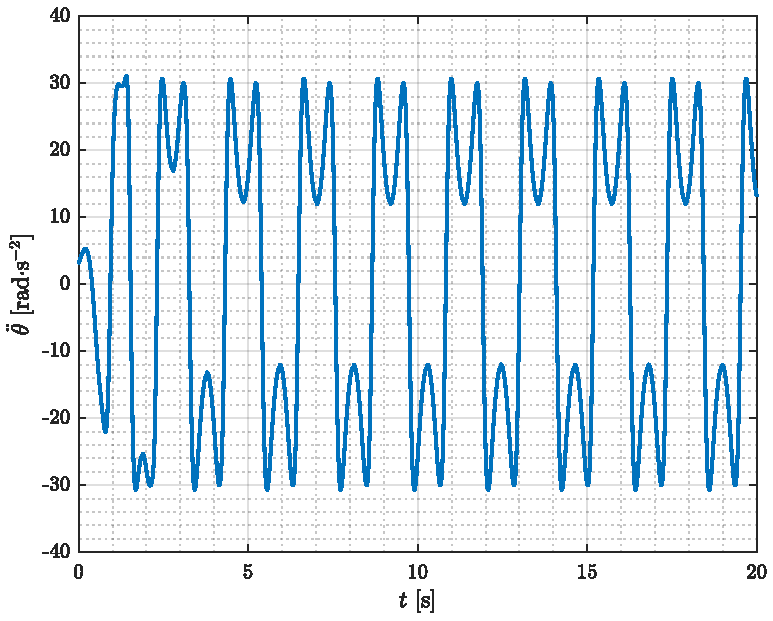
\includegraphics[width=.6\textwidth]{figures/thetaDotDot_1_noConX}
%  \caption{thetaDotDot1noConX}
%  \label{fig:thetaDotDot_1_noConX}
%\end{figure}


\subsection{Sign-Based Energy Control}
There are other ways to satisfy \autoref{eq:lyapunovDerivativeControlled2} than the control law suggested in \autoref{eq:accControlLaw}. To achieve maximal actuation a sign-function can be used to determine the direction of actuation along with a gain $k$ to adjust for the limits of the actuator,
\begin{flalign}
  && a_c &= k\ \mathrm{sgn}(-E_\Delta \cos \theta \dot{\theta})  \ \ \ ,  \hspace{4cm}  &&&  \label{eq:accControlLaw2} 
\end{flalign}
where sgn is redefined to be one if it outputs zero, to avoid no actuation when starting at stable equilibrium. The gain is tuned to $k = 2.7$ in the following simulation. Looking at the energy in \autoref{fig:Edelta_2_noConX} this strategy seems to work really well. From the phase plot in \autoref{fig:phase_2_noConX} it is evident that a near perfect heteroclinic orbit is reached.
\begin{figure}[H]
  \hspace{-10pt}
  \captionbox
  {
    Using maximum actuation in the appropriate direction drives the energy error to zero and keeps it there.
    \label{fig:Edelta_2_noConX}
  }
  {
    \hspace{-1cm}
    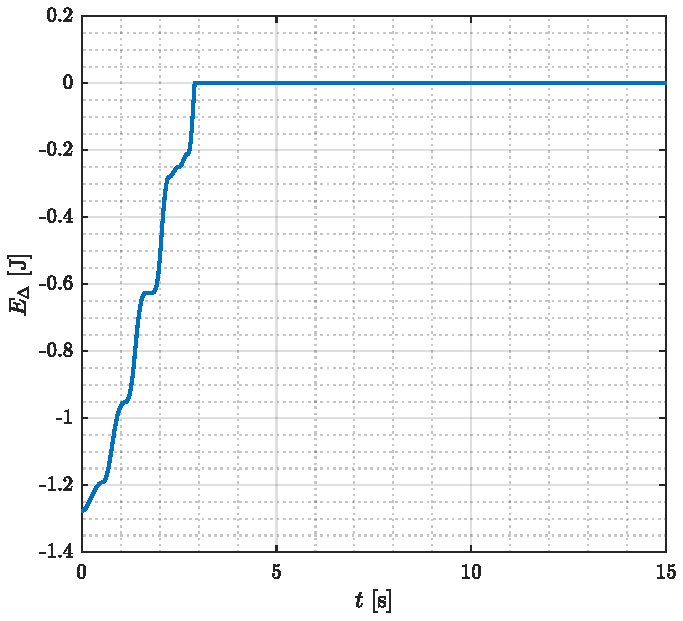
\includegraphics[width=.46\textwidth]{figures/Edelta_2_noConX}
  }
  \hspace{20pt}
  \captionbox 
  {
    The heteroclinic orbit is reached very accurately.
    \label{fig:phase_2_noConX}
  }
  {
    \hspace{-1cm}
    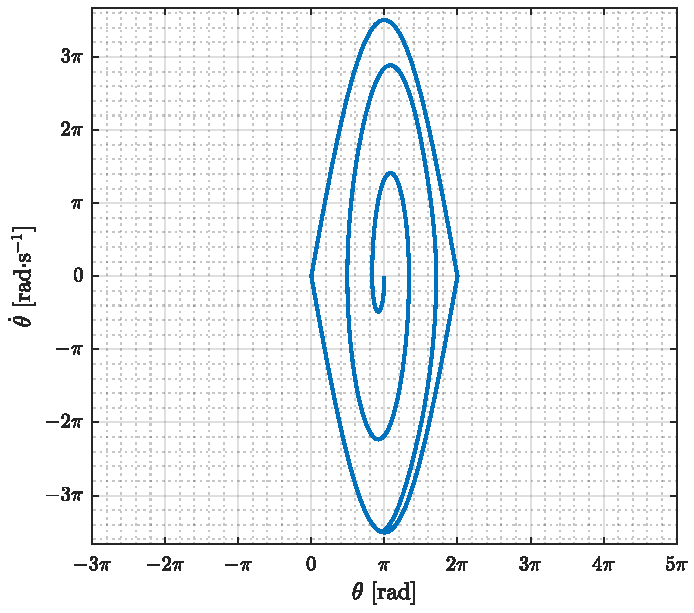
\includegraphics[width=.46\textwidth]{figures/phase_2_noConX}
  }  
\end{figure}
%
In \autoref{fig:ani_2_noConX} however, while the angle reaches the equilibrium as closely as possible without overshooting, this control law, as with the previous, does not account for position of the cart.
%
\begin{figure}[H]
  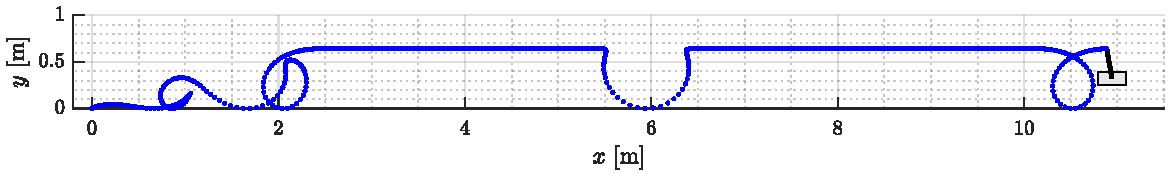
\includegraphics[width=1\textwidth]{figures/ani_2_noConX}
  \caption{The cart drifts as before, since the controller is only concerned with the energy of the pendulum.}
  \label{fig:ani_2_noConX}
\end{figure}
%
However, the bigger problem with this control law is obvious from \autoref{fig:ia_2_noConX}, where excessive switching shows on the control output. This actuation behavior is not feasible in a real system and attempted implementation will cause chattering resulting in unwanted behavior and wear of the motor.
%
\begin{figure}[H]
  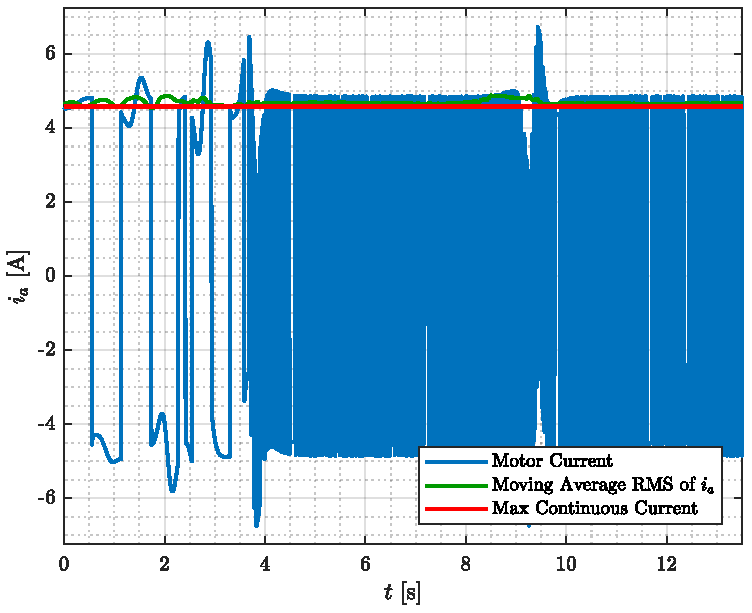
\includegraphics[width=.52\textwidth]{figures/ia_2_noConX}
  \caption{The sign-function in the control law causes excessive switching in the output, thus, the design is not feasible for a real system implementation.}
  \label{fig:ia_2_noConX}
\end{figure}
%
%\begin{figure}[H]
%  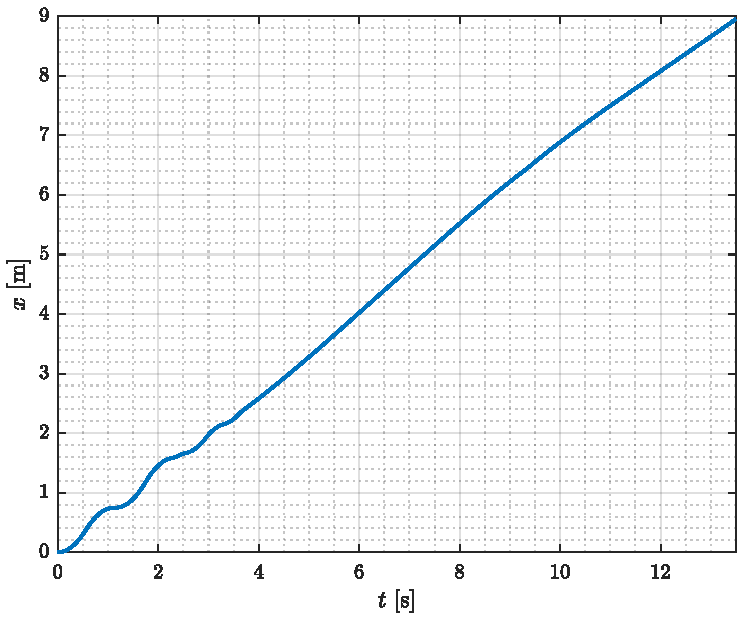
\includegraphics[width=.6\textwidth]{figures/x_2_noConX}
%  \caption{x2noConX}
%  \label{fig:x_2_noConX}
%\end{figure}
%\begin{figure}[H]
%  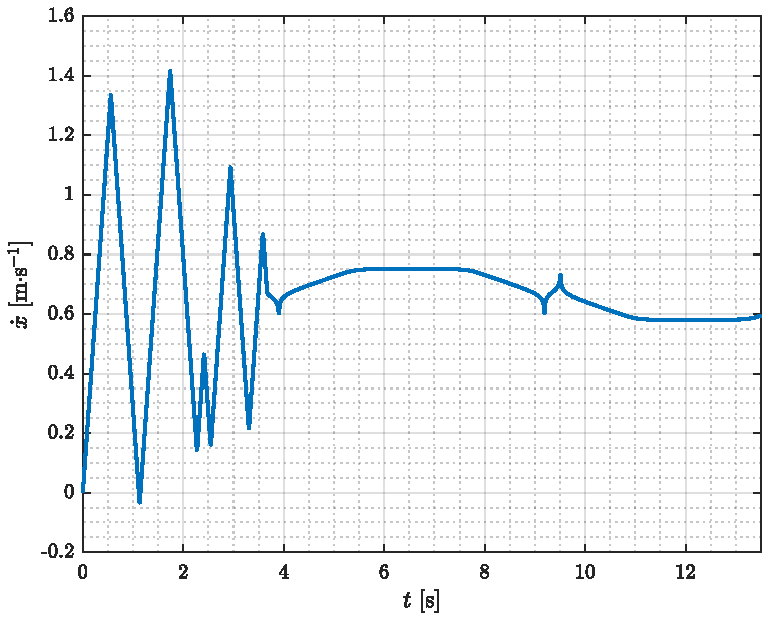
\includegraphics[width=.6\textwidth]{figures/xDot_2_noConX}
%  \caption{xDot2noConX}
%  \label{fig:xDot_2_noConX}
%\end{figure}
%\begin{figure}[H]
%  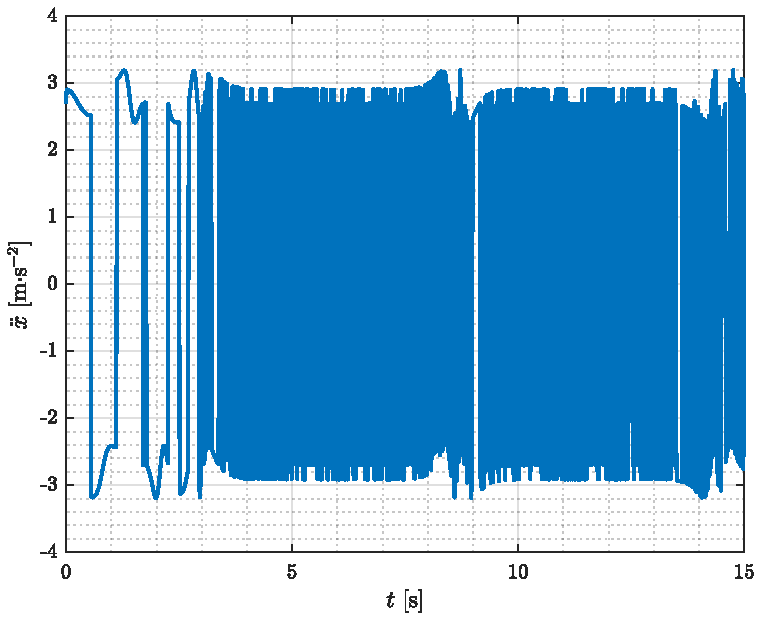
\includegraphics[width=.6\textwidth]{figures/xDotDot_2_noConX}
%  \caption{xDotDot2noConX}
%  \label{fig:xDotDot_2_noConX}
%\end{figure}
%\begin{figure}[H]
%  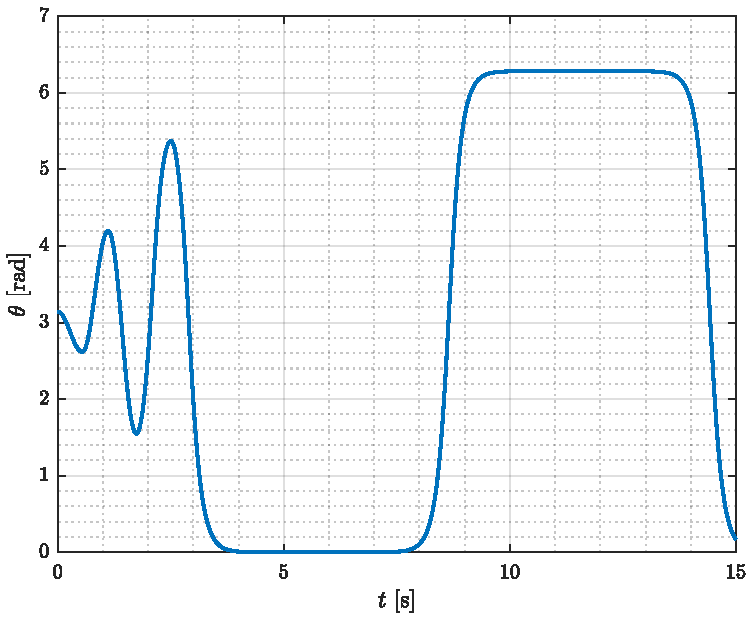
\includegraphics[width=.6\textwidth]{figures/theta_2_noConX}
%  \caption{theta2noConX}
%  \label{fig:theta_2_noConX}
%\end{figure}
%\begin{figure}[H]
%  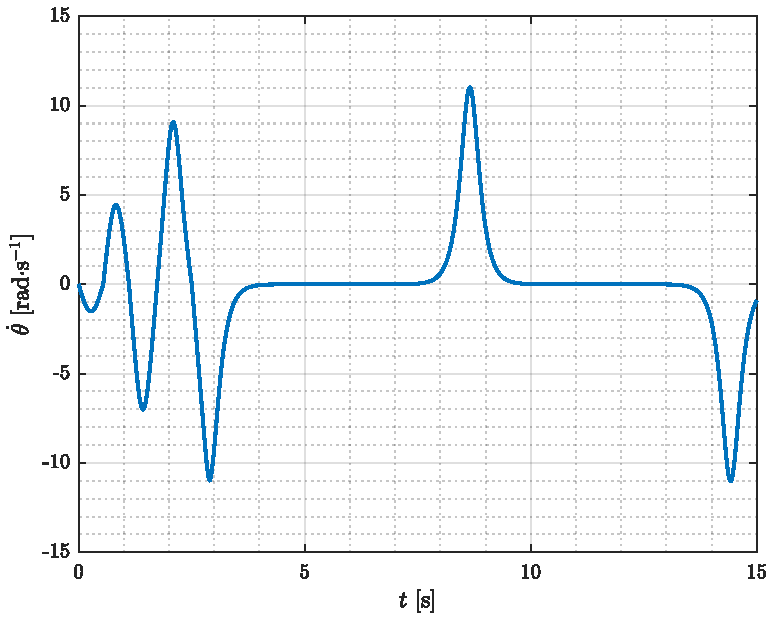
\includegraphics[width=.6\textwidth]{figures/thetaDot_2_noConX}
%  \caption{thetaDot2noConX}
%  \label{fig:thetaDot_2_noConX}
%\end{figure}
%\begin{figure}[H]
%  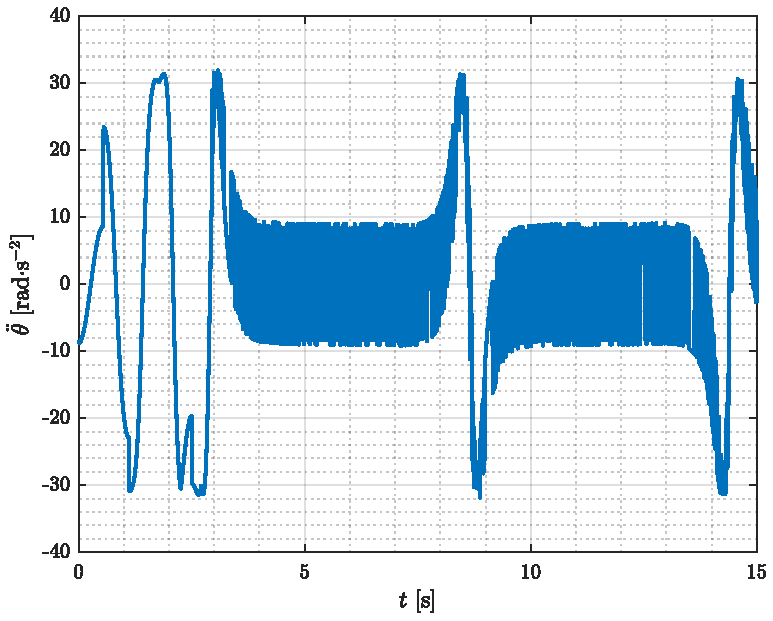
\includegraphics[width=.6\textwidth]{figures/thetaDotDot_2_noConX}
%  \caption{thetaDotDot2noConX}
%  \label{fig:thetaDotDot_2_noConX}
%\end{figure}
%
%
%
It is possible to implement a less aggressive version of this idea by using a saturation function to approximate the sign function around zero,
\begin{flalign}
  && a_c &= k\ \mathrm{sat}(-\tfrac{1}{\varepsilon}E_\Delta \cos \theta \dot{\theta})  \ \ \ ,  \hspace{4cm}  &&&  \label{eq:accControlLaw2_2} 
\end{flalign}
where $\varepsilon$ decides the slope of the saturation function around zero,
\begin{flalign}
  &&\text{sat}\left( \frac{c}{\varepsilon} \right) &=
  \begin{cases}
    \ \ \frac{c}{\varepsilon}                             &, \ \ \ \ \mathrm{if} \ | \frac{c}{\varepsilon} | \leq 1 \\
    \ \ \mathrm{sgn}\left( \frac{c}{\varepsilon} \right)  &, \ \ \ \ \mathrm{if} \ | \frac{c}{\varepsilon} |  >   1 \ \ \ ,
  \end{cases} &&& 
  \label{eq:satuationFunction1}
\end{flalign}
where $c$ is an input to the sat-function.
In the simulation $k = 2.7$ as before and $\varepsilon = 0.01$ to avoid excessive switching while maintaining a relatively close approximation of the sign-function. This control strategy achieves the energy reference in about three seconds, \autoref{fig:Edelta_3_noConX}, as is the case of the sign strategy, \autoref{fig:Edelta_2_noConX}. Further, from \autoref{fig:phase_3_noConX}, the system still reaches a near perfect heteroclinic orbit.
%
\begin{figure}[H]
  \hspace{-10pt}
  \captionbox
  {
    The approximation of the sign approach using a saturation function shows no loss in performance when comparing the energy error.
    \label{fig:Edelta_3_noConX}
  }
  {
    \hspace{-1cm}
    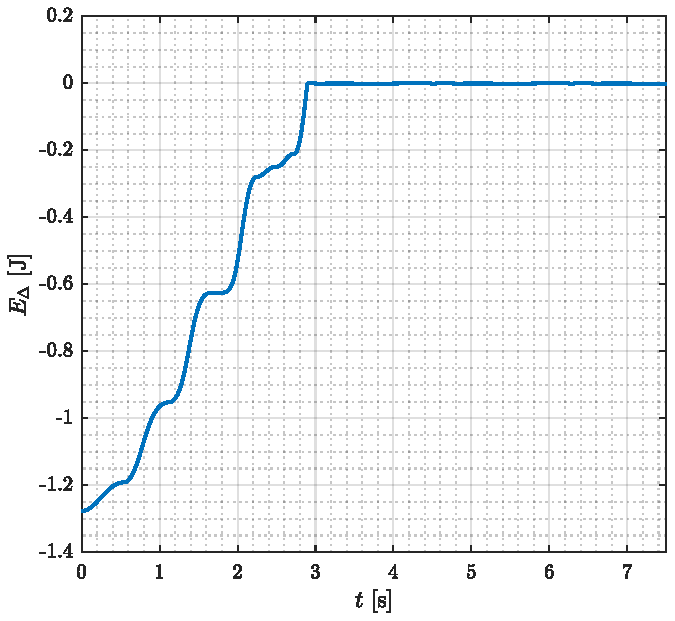
\includegraphics[width=.46\textwidth]{figures/Edelta_3_noConX}
  }
  \hspace{20pt}
  \captionbox 
  {
    The heteroclinic orbit is still reached, however, with a more realistic trajectory at the approach of the equilibrium points.
    \label{fig:phase_3_noConX}
  }
  {
    \hspace{-1cm}
    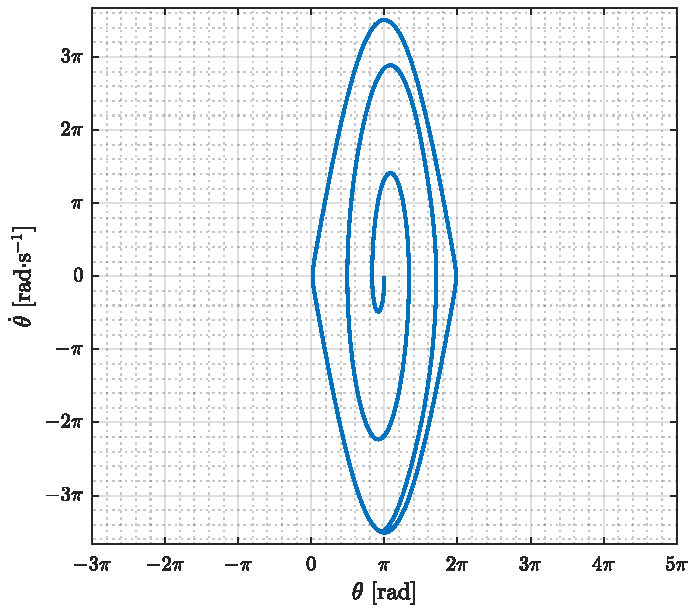
\includegraphics[width=.46\textwidth]{figures/phase_3_noConX}
  }  
\end{figure}
%
The cart still drifts as expected, see \autoref{fig:ani_3_noConX}, and the equilibrium points are maintained for shorter durations, which is expected with less control switching.
%
\begin{figure}[H]
  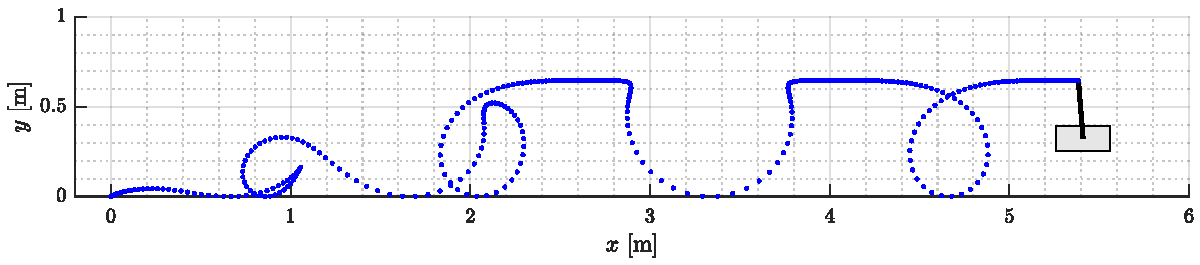
\includegraphics[width=.7\textwidth]{figures/ani_3_noConX}
  \caption{This strategy performs well. The drifting problem is solved later.}
  \label{fig:ani_3_noConX}
\end{figure}
%
The excessive switching on the control output is successfully avoided, see \autoref{fig:ia_3_noConX}, resulting in a much more realistic control signal compared to that in \autoref{fig:ia_2_noConX}.
%
\begin{figure}[H]
  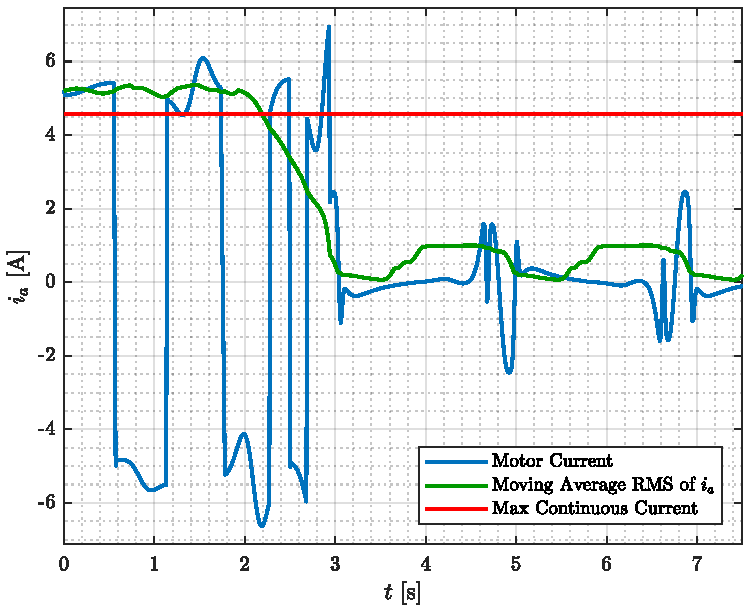
\includegraphics[width=.52\textwidth]{figures/ia_3_noConX}
  \caption{The control signal using the saturation approximation of the sign-function is much more realistic for implementation.}
  \label{fig:ia_3_noConX}
\end{figure}
The next section explores an other approach based on the same general idea and motivation.
%
%
%\begin{figure}[H]
%  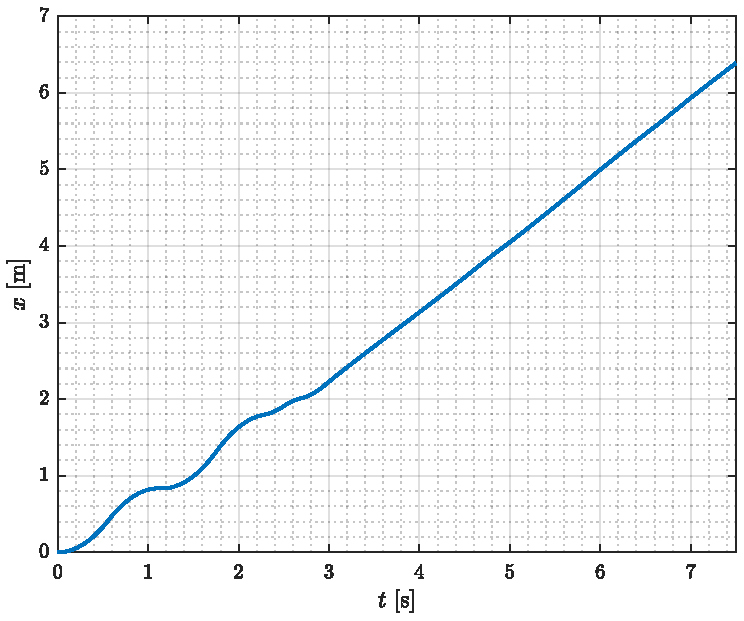
\includegraphics[width=.6\textwidth]{figures/x_3_noConX}
%  \caption{x3noConX}
%  \label{fig:x_3_noConX}
%\end{figure}
%\begin{figure}[H]
%  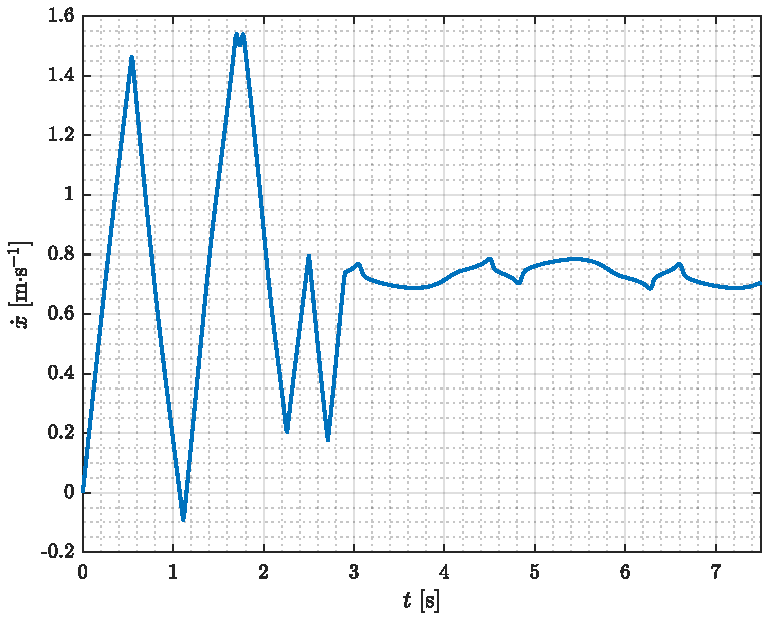
\includegraphics[width=.6\textwidth]{figures/xDot_3_noConX}
%  \caption{xDot3noConX}
%  \label{fig:xDot_3_noConX}
%\end{figure}
%\begin{figure}[H]
%  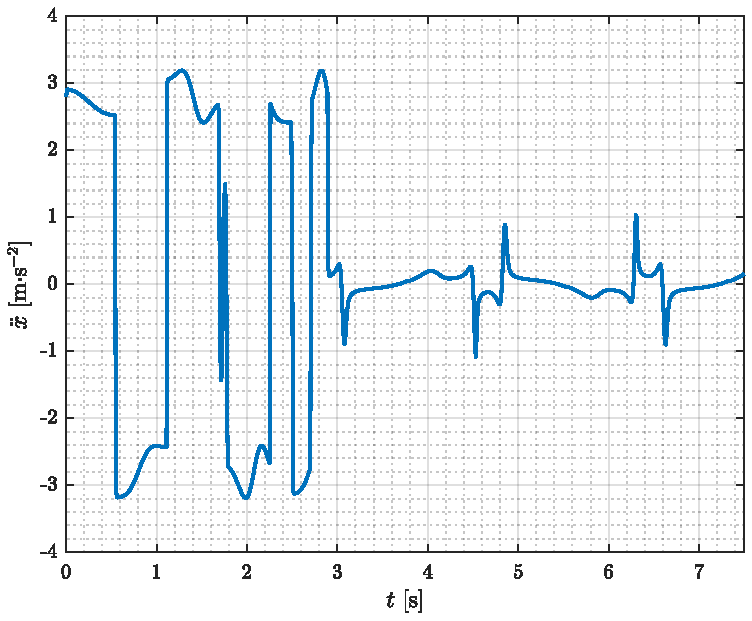
\includegraphics[width=.6\textwidth]{figures/xDotDot_3_noConX}
%  \caption{xDotDot3noConX}
%  \label{fig:xDotDot_3_noConX}
%\end{figure}
%\begin{figure}[H]
%  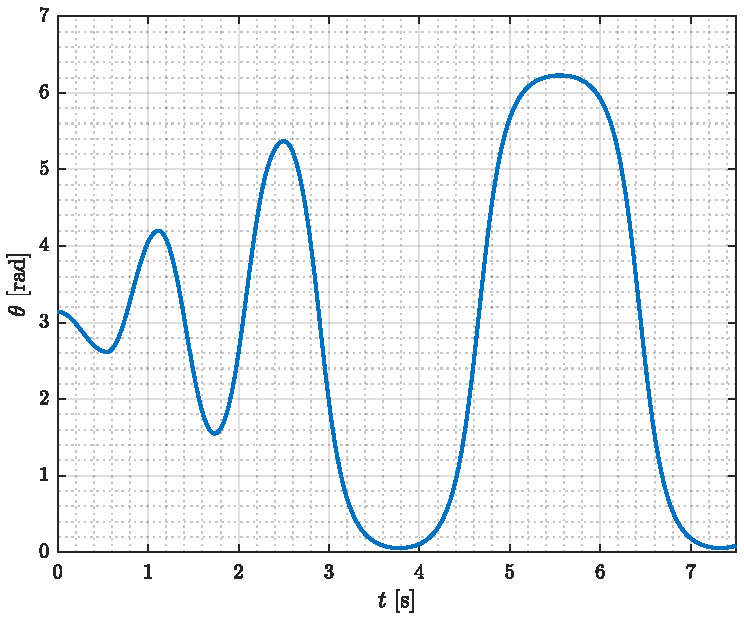
\includegraphics[width=.6\textwidth]{figures/theta_3_noConX}
%  \caption{theta3noConX}
%  \label{fig:theta_3_noConX}
%\end{figure}
%\begin{figure}[H]
%  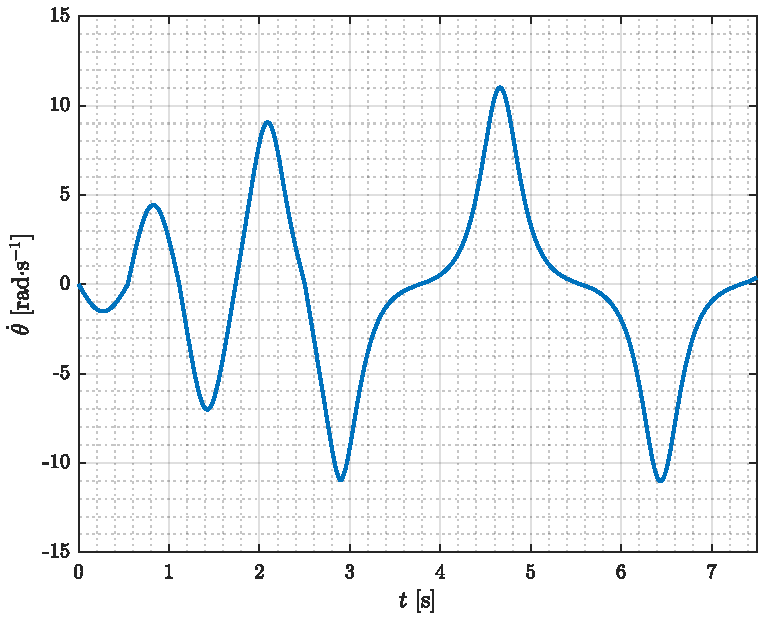
\includegraphics[width=.6\textwidth]{figures/thetaDot_3_noConX}
%  \caption{thetaDot3noConX}
%  \label{fig:thetaDot_3_noConX}
%\end{figure}
%\begin{figure}[H]
%  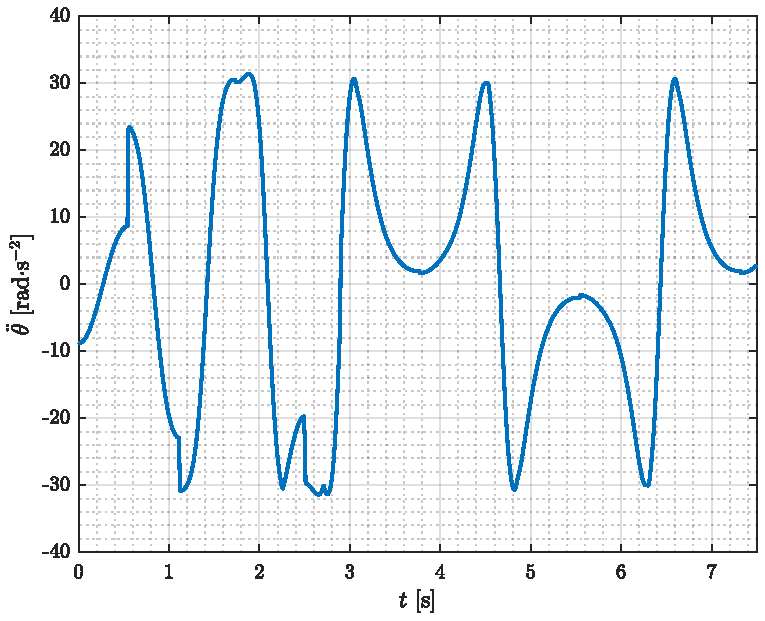
\includegraphics[width=.6\textwidth]{figures/thetaDotDot_3_noConX}
%  \caption{thetaDotDot3noConX}
%  \label{fig:thetaDotDot_3_noConX}
%\end{figure}

\subsection{Saturation Based Energy Control}
An other strategy to avoid the excessive switching of the sign-controller is to combine saturation and sign functions in the following manner,
\begin{flalign}
  && a_c &= \mathrm{sat}(-k E_\Delta \mathrm{sgn}(\cos \theta \dot{\theta}))  \ \ \ ,  \hspace{4cm}  &&&  \label{eq:accControlLaw3} 
\end{flalign}
where the sat-function saturates at the maximum/minimum allowed acceleration. The known limitation is $i_{max} = 4.58$ as stated in \autoref{table:systemParameters}, from which the maximum control, $u$, can be calculated,
\begin{flalign}
  && u_{max} &=  \frac{k_{\tau}}{r} \ \ \ ,  \hspace{4cm}  &&&  \label{eq:maxU} 
\end{flalign}
and finally, by disregarding the pendulum behavior and cart friction from the dynamics in \autoref{eq:energyDerivedDynamicEquation1},
\begin{flalign}
  && a_{max} &= \frac{u_{max}}{M+m} \ \ \ .  \hspace{4cm}  &&&  \label{eq:maxAcc} 
\end{flalign}
As this is a crude estimation $0.2$ is subtracted from the estimated $a_{max}$ in following simulations to stay within the actuation limits. The saturation function is then,
\begin{flalign}
  &&\text{sat}(c) &=
  \begin{cases}
    \ \ c                          &, \ \ \ \ \mathrm{if} \ | c | \leq a_{max} \\
    \ \ \mathrm{sgn}( c )\ a_{max}  &, \ \ \ \ \mathrm{if} \ | c |  >   a_{max} \ \ \ ,
  \end{cases} &&& 
  \label{eq:satuationFunction2}
\end{flalign}
where $c$ is the input to the sat-function. Again, the sign function is redefined to one in cases where it obtains a zero value.
Choice of $k$ in \autoref{eq:accControlLaw3} decides how aggressive the controller should be. Larger values of $k$ drives the control into saturation faster thus actuating more like the sign-based controller in \autoref{eq:accControlLaw2}. At lower values of $k$ the operation will not reach saturation as fast thus behaving more like the first energy based controller in \autoref{eq:accControlLaw}. For an effective swing up behavior $k=200$ is used, thus approaching the behavior of the sign-based controller, which makes sense as this is the theoretically ideal solution.\\
The performance in \autoref{fig:Edelta_4_noConX} is similar to that in \autoref{fig:Edelta_3_noConX} and again the system reaches a near perfect heteroclinic orbit in \autoref{fig:phase_4_noConX}.
%
\begin{figure}[H]
  \hspace{-10pt}
  \captionbox
  {
    This strategy is closely related to the saturation approximation of the sign approach. This fact shows here in the energy error plot where the performances of the two approaches are almost indistinguishable.
    \label{fig:Edelta_4_noConX}
  }
  {
    \hspace{-1cm}
    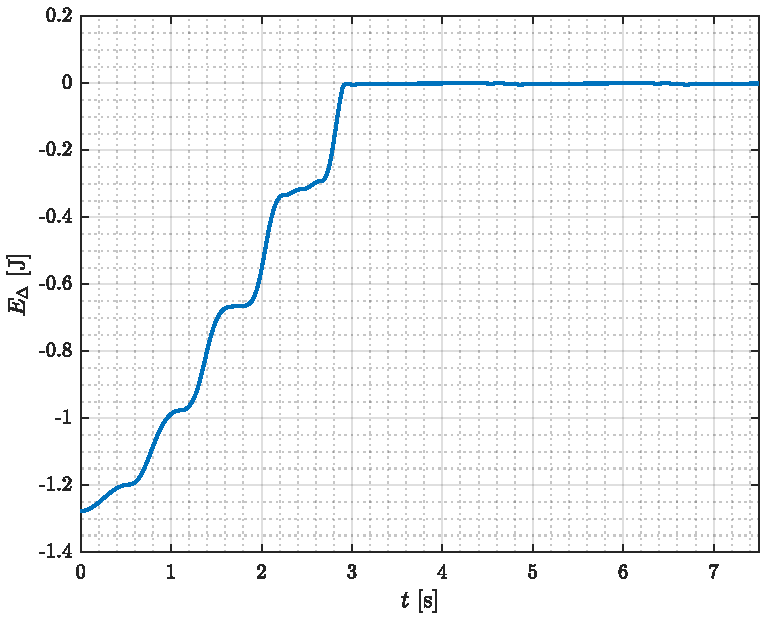
\includegraphics[width=.46\textwidth]{figures/Edelta_4_noConX}
  }
  \hspace{20pt}
  \captionbox 
  {
    In the phase portrait the heteroclinic orbit is still reached, however a small difference is seen in the trajectory right before reaching orbit.
    \label{fig:phase_4_noConX}
  }
  {
    \hspace{-1cm}
    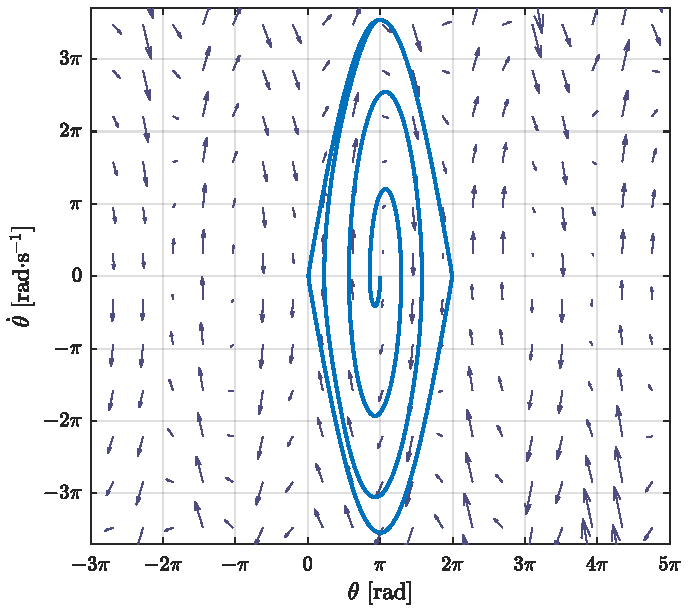
\includegraphics[width=.46\textwidth]{figures/phase_4_noConX}
  }  
\end{figure}
%
The overall behavior also closely mimics that of \autoref{fig:ani_3_noConX} as seen in \autoref{fig:ani_4_noConX}.
\begin{figure}[H]
  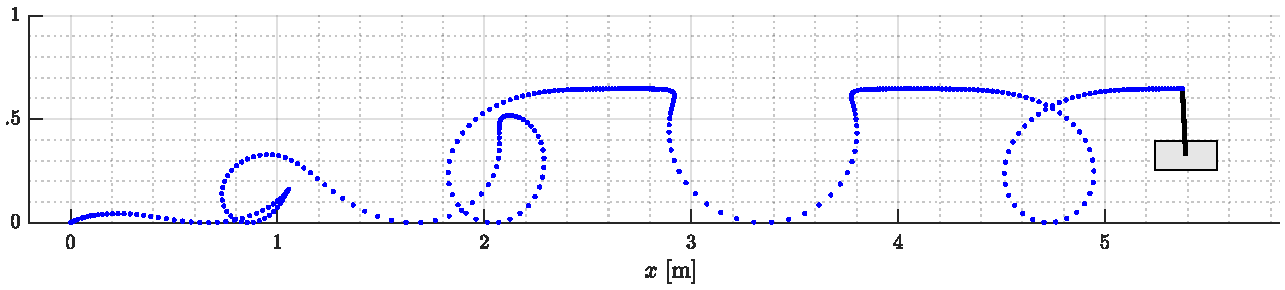
\includegraphics[width=.7\textwidth]{figures/ani_4_noConX}
  \caption{The cart drifts as expected and the overall behavior is very similar to the approximated sign approach.}
  \label{fig:ani_4_noConX}
\end{figure}
%
There is however a slight difference in the control signal. In \autoref{fig:ia_4_noConX} less switching occurs compared to \autoref{fig:ia_3_noConX}. 
\begin{figure}[H]
  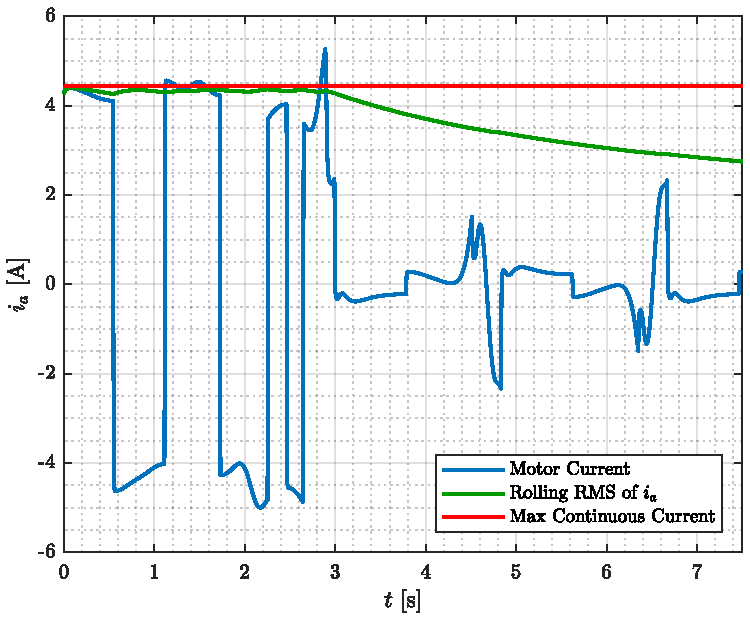
\includegraphics[width=.52\textwidth]{figures/ia_4_noConX}
  \caption{Slightly less switching occurs when compared to the previous approach, making this approach a viable candidate.}
  \label{fig:ia_4_noConX}
\end{figure}
%
Two of the four investigated controller designs are deemed good candidates, namely \autoref{eq:accControlLaw2_2} and \autopageref{eq:accControlLaw3}. The problem of controlling the cart position still remains. In the following, performances of the two control law candidates are compared as they are subjected to the disturbance caused by added control on the cart position and velocity.
%
%
%\begin{figure}[H]
%  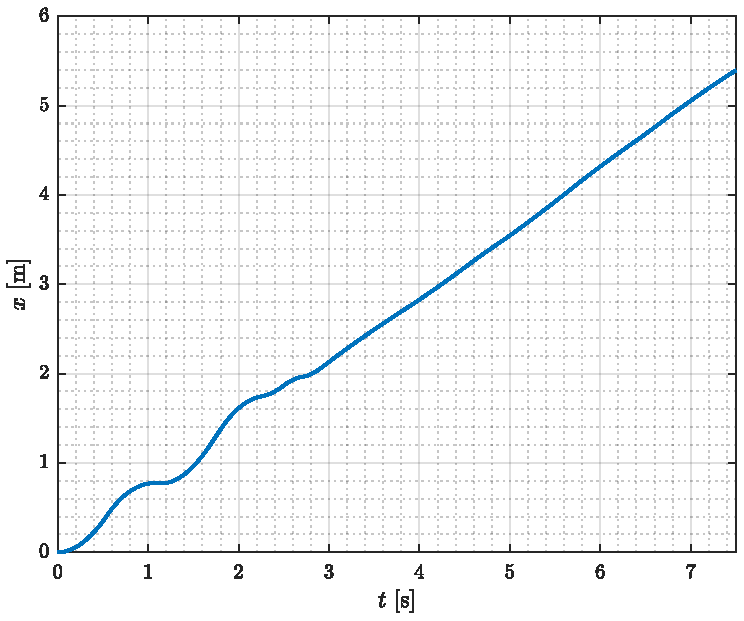
\includegraphics[width=.6\textwidth]{figures/x_4_noConX}
%  \caption{x4noConX}
%  \label{fig:x_4_noConX}
%\end{figure}
%\begin{figure}[H]
%  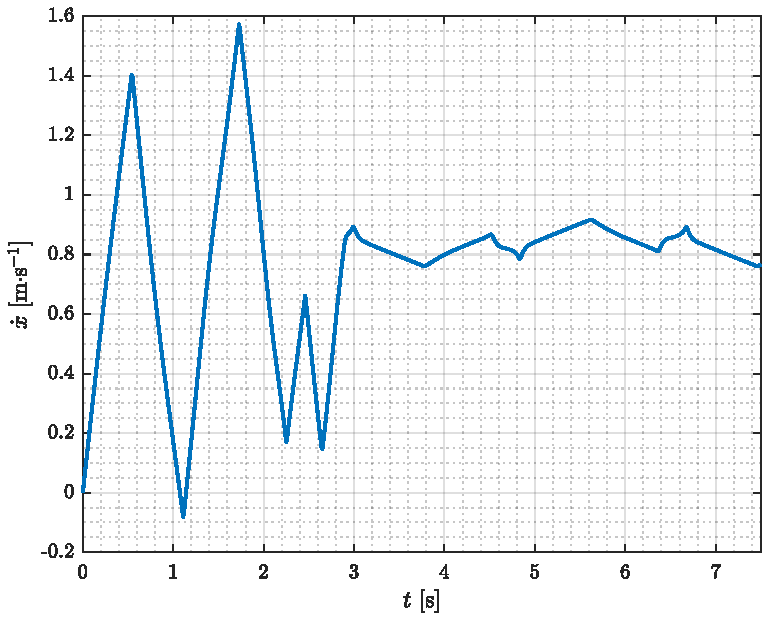
\includegraphics[width=.6\textwidth]{figures/xDot_4_noConX}
%  \caption{xDot4noConX}
%  \label{fig:xDot_4_noConX}
%\end{figure}
%\begin{figure}[H]
%  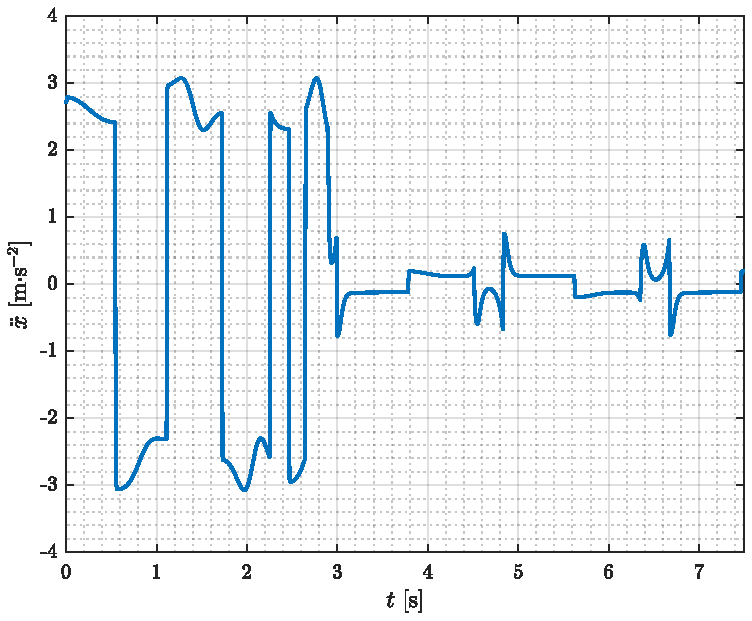
\includegraphics[width=.6\textwidth]{figures/xDotDot_4_noConX}
%  \caption{xDotDot4noConX}
%  \label{fig:xDotDot_4_noConX}
%\end{figure}
%\begin{figure}[H]
%  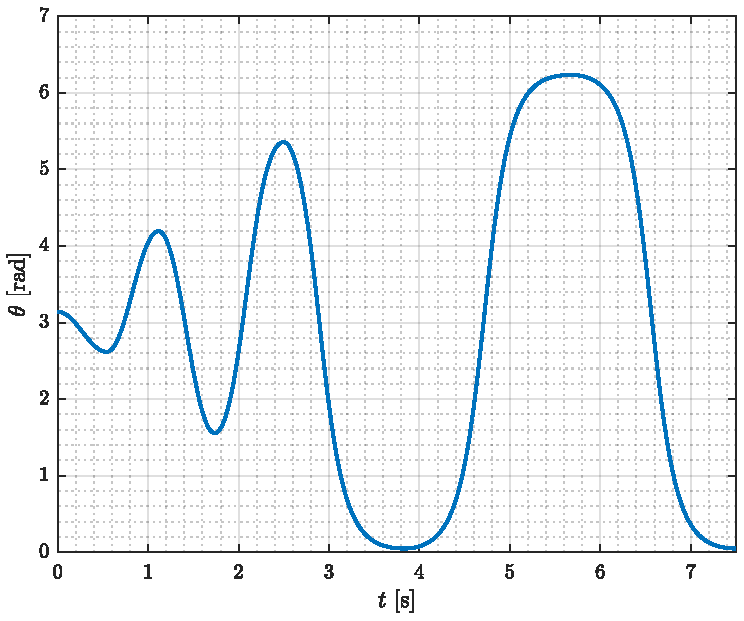
\includegraphics[width=.6\textwidth]{figures/theta_4_noConX}
%  \caption{theta4noConX}
%  \label{fig:theta_4_noConX}
%\end{figure}
%\begin{figure}[H]
%  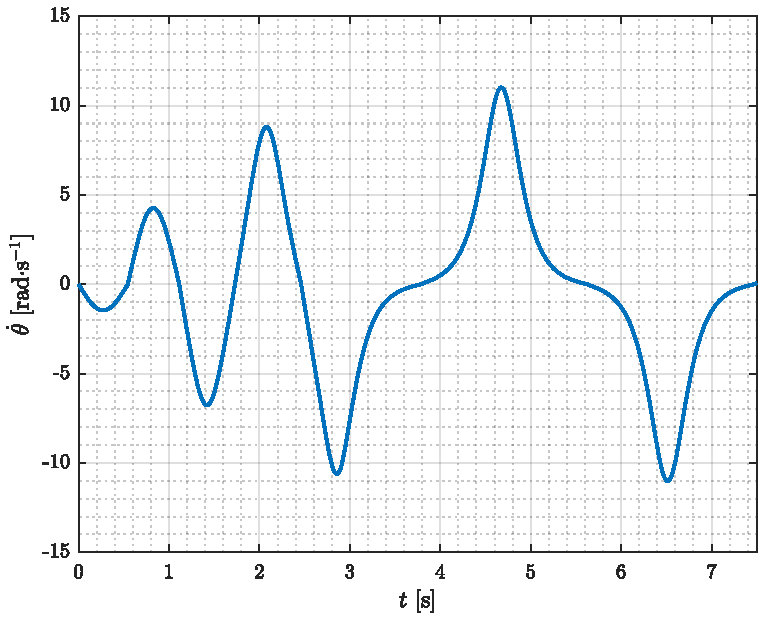
\includegraphics[width=.6\textwidth]{figures/thetaDot_4_noConX}
%  \caption{thetaDot4noConX}
%  \label{fig:thetaDot_4_noConX}
%\end{figure}
%\begin{figure}[H]
%  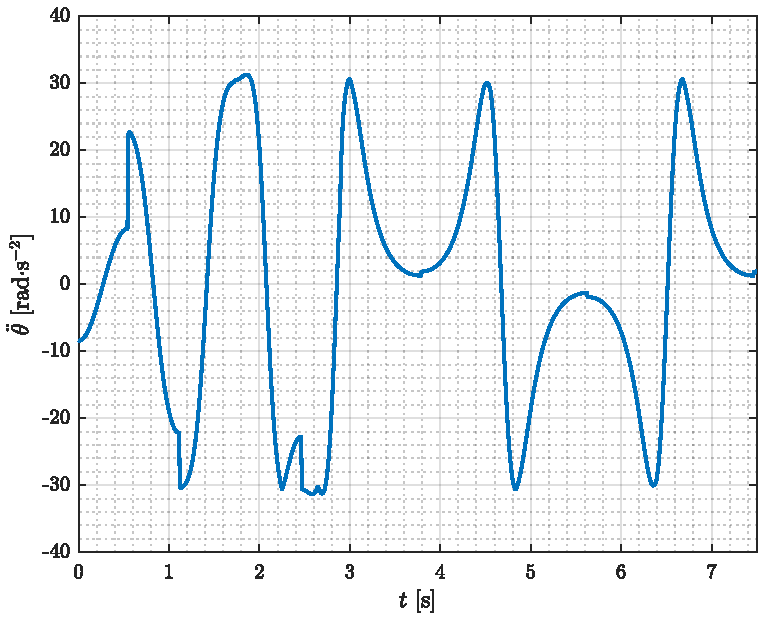
\includegraphics[width=.6\textwidth]{figures/thetaDotDot_4_noConX}
%  \caption{thetaDotDot4noConX}
%  \label{fig:thetaDotDot_4_noConX}
%\end{figure}

\subsection{Cart Position and Velocity Control}
To solve the cart drifting problem along $x$ a linear controller is designed and added to the control law,
\begin{flalign}
  && a_c &= \psi(x_1,x_3) + v(x_2,x_4) \ \ \ ,  \hspace{4cm}  &&&  \label{eq:combiControl} 
\end{flalign}
where $\psi(x_1,x_3)$ is the energy controller and $v(x_2,x_4)$ is the linear controller. While these two controllers depend on different states, they still influence and act as unmodeled disturbances on one another. The position and velocity control, $v(x_2,x_4)$, adds and subtracts energy to the pendulum, therefore could cause the energy controller, $\psi(x_1,x_3)$, to overshoot. One solution to this potential problem could be to slightly lower the energy reference. However, swing-up is often designed with a slightly higher energy reference such that the catch controller has some entry velocity at the unstable equilibrium.\\
With these considerations in mind, the design of $v(x_2,x_4)$ is proceeded. Considering the cart without friction and assuming any influence of the pendulum dynamics and the energy control to be unmodeled disturbances of the system. This reduces the model to the mechanical drawing seen in \autoref{fig:mechanicalDrawingSimple}.
%
\begin{figure}[H]
  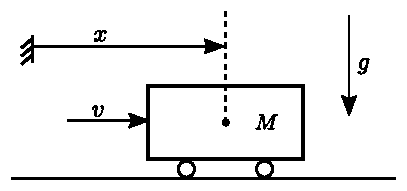
\includegraphics[width=.35\textwidth]{figures/mechanicalDrawingSimple}
  \caption{mechanicalDrawingSimple}
  \label{fig:mechanicalDrawingSimple}
\end{figure}
%
The dynamics are then,
\begin{flalign}
  && M \ddot{x} &=  v \ \ \ ,  \hspace{4cm}  &&&  \label{eq:simpleDynamics} 
\end{flalign}
and selecting new states $ [\ x_1\ \ x_2\ ]^\mathrm{T} = [\ x\ \ \dot{x}\ ]^\mathrm{T} $, the linear state space is,
\begin{flalign}
  &&
  \begin{bmatrix}
    \dot{x_1} \\
    \dot{x_2}
  \end{bmatrix}
  &=
  \underbrace{
    \begin{bmatrix}
      0 & 1 \\
      0 & 0
    \end{bmatrix}
  }_{A}
  \begin{bmatrix}
    x_1 \\
    x_2
  \end{bmatrix}
  +
  \underbrace{
    \begin{bmatrix}
      0 \\
      \tfrac{1}{M}
    \end{bmatrix}
  }_{B}
  v
  \label{eq:simpleLinearStateSpace} \ \ \ . &&&
\end{flalign}
%
The closed loop poles are placed in $p = [\ -1\ -2 \ ] $ using matlab \textit{place()}-command to obtain linear feedback gains, $\vec{k_1} = [\ 10.5460\ \ 15.8190\ ]$, resulting in the controller,
\begin{flalign}
  && v &= -\vec{k_1} \vec{x} \ \ \ ,  \hspace{4cm}  &&&  \label{eq:linearFeedbackSimple} 
\end{flalign}
where $\vec{x} = [\ x\ \ \dot{x}\ ]^\mathrm{T}$, such that,
\begin{flalign}
  && v(x_2,x_4) &= -\vec{k_1}  [\ x_2\ \ x_4\ ]^\mathrm{T} \ \ \ ,  \hspace{4cm}  &&&  \label{eq:linearFeedbackSimple2} 
\end{flalign}
in therms of the full system. This control is added to both of the considered energy control approaches and simulations are run without changing any previously designed gains.\\
\autoref{fig:Edelta_3_conX} shows the energy difference in the approximated sign approach while \autoref{fig:Edelta_4_conX} shows the sat-based approach. The approximated sign control approaches the reference slightly faster, however both reaches the reference at the same time.
%
\begin{figure}[H]
  \hspace{-10pt}
  \captionbox
  {
    The sign approximation approach still reaches zero energy error, however a second slower due to the disturbance form the linear control.
    \label{fig:Edelta_3_conX}
  }
  {
    \hspace{-1cm}
    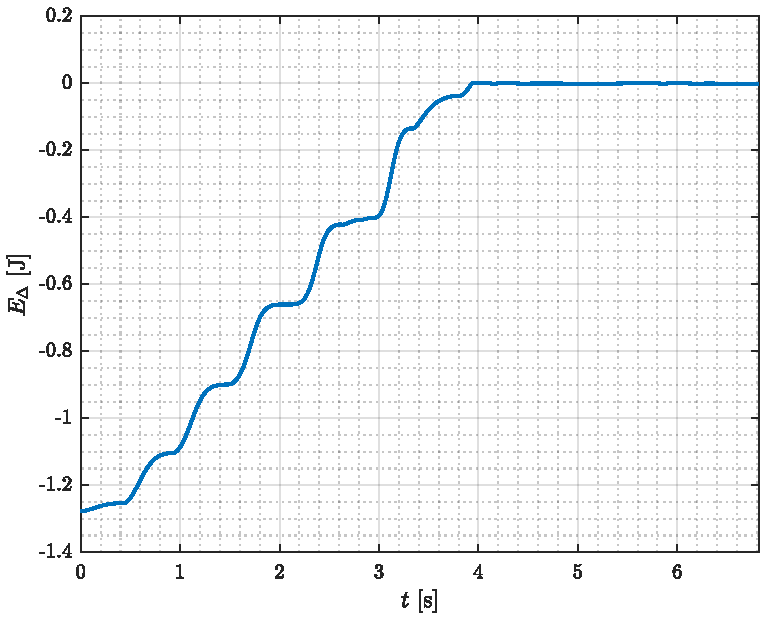
\includegraphics[width=.46\textwidth]{figures/Edelta_3_conX}
  }
  \hspace{20pt}
  \captionbox 
  {
    The saturation based controller reaches the reference in about four seconds as well. However, the curve is steeper as it approaches the reference, indicating less energy before reaching orbit.
    \label{fig:Edelta_4_conX}
  }
  {
    \hspace{-1cm}
    \includegraphics[width=.46\textwidth]{figures/Edelta_4_conX}
  }  
\end{figure}
%
In the phase portraits, see \autoref{fig:phase_3_conX} and \ref{fig:phase_4_conX}, both control strategies reaches the heteroclinic orbit. However the approximated sign approach comes slightly closer in the swing preceding the orbit. If it is close enough that a catch controller could catch it, one swing could be saved.
\begin{figure}[H]
  \hspace{-10pt}
  \captionbox
  {
    As indicated by the energy error, extra time and thus swing is needed to reach orbit when influenced by the linear control.
    \label{fig:phase_3_conX}
  }
  {
    \hspace{-1cm}
    \includegraphics[width=.46\textwidth]{figures/phase_3_conX}
  }
  \hspace{20pt}
  \captionbox 
  {
    In the phase plane, the behavior of the two approaches are again very similar. However, the tendency of the saturation based controller to approach equilibrium slower is amplified after influence of the linear control.
    \label{fig:phase_4_conX}
  }
  {
    \hspace{-1cm}
    \includegraphics[width=.46\textwidth]{figures/phase_4_conX}
  }  
\end{figure}
%
This fact is also seen in \autoref{fig:ani_3_conX} where the trace of the swing preceding the heteroclinic orbit reaches higher than in \autoref{fig:ani_4_conX}. These figures also show that the linear control of the cart position and velocity successfully keeps the system within the accessible operating region of the real system.
%
\begin{figure}[H]
  \hspace{-10pt}
  \captionbox
  {
    The linear control successfully keeps the cart around zero while the energy control approaches the unstable equilibrium.
    \label{fig:ani_3_conX}
  }
  {
    \hspace{-1cm}
    \includegraphics[width=.46\textwidth]{figures/ani_3_conX}
  }
  \hspace{20pt}
  \captionbox 
  {
    The performance of the approximated sign is slightly better in the swing prior to reaching the heteroclinic orbit.
    \label{fig:ani_4_conX}
  }
  {
    \hspace{-1cm}
    \includegraphics[width=.46\textwidth]{figures/ani_4_conX}
  }  
\end{figure}
%
\autoref{fig:ia_3_conX} shows the actuation of the approximated sign approach, where the added linear control has caused less switching compared to \autoref{fig:ia_3_noConX}. In fact, both control strategies show very similar output when comparing to \autoref{fig:ia_4_conX}. In both cases the RMS is lower than before the added linear controller. This could be tuned more tightly, but is left as a margin for now, with the possibility of further tuning during implementation.
%
\begin{figure}[H]
  \hspace{-10pt}
  \captionbox
  {
    The control signal for the approximated sign approach switches less after the added linear control.
    \label{fig:ia_3_conX}
  }
  {
    \hspace{-1cm}
    \includegraphics[width=.46\textwidth]{figures/ia_3_conX}
  }
  \hspace{20pt}
  \captionbox 
  {
    The two approaches share very similar control signals, which is to be expected as both methods are very similar at large control values.
    \label{fig:ia_4_conX}
  }
  {
    \hspace{-1cm}
    \includegraphics[width=.46\textwidth]{figures/ia_4_conX}
  }  
\end{figure}
%
\autoref{fig:x_3_conX} and \ref{fig:x_4_conX} show the position approaching zero as the energy control settles, which is ideal, as it means the energy controllers still have room to operate without fighting the linear feedback controller too much. Similarly, the oscillations around zero are necessary for the energy controller to keep its reference.
%
\begin{figure}[H]
  \hspace{-10pt}
  \captionbox
  {
    This shows the added linear feedback control oscilating around zero, allowing the energy controller room to operate.
    \label{fig:x_3_conX}
  }
  {
    \hspace{-1cm}
    \includegraphics[width=.4\textwidth]{figures/x_3_conX}
  }
  \hspace{20pt}
  \captionbox 
  {
    The saturation based controller keeps the cart closer to zero, suggesting less actuation from the energy control.
    \label{fig:x_4_conX}
  }
  {
    \hspace{-1cm}
    \includegraphics[width=.4\textwidth]{figures/x_4_conX}
  }  
\end{figure}
The same is seen for the velocity in \autoref{fig:xDot_3_conX} and \ref{fig:xDot_4_conX}. These four graphs are simulated over longer time to show that the linear controller reaches its reference.
\begin{figure}[H]
  \hspace{-10pt}
  \captionbox
  {
    Zero velocity is obtained quite effectively after the energy reference is reached.
    \label{fig:xDot_3_conX}
  }
  {
    \hspace{-1cm}
    \includegraphics[width=.4\textwidth]{figures/xDot_3_conX}
  }
  \hspace{20pt}
  \captionbox 
  {
    Again, both control strategies behave very similarly.
    \label{fig:xDot_4_conX}
  }
  {
    \hspace{-1cm}
    \includegraphics[width=.4\textwidth]{figures/xDot_4_conX}
  }  
\end{figure}

This concludes the design of swing-up control. Though some small advantages are seen in the approximated sign control over the saturation based, both strategies are still viable options, therefore both are eventually implemented and tested.
%
%
%
%\begin{figure}[H]
%  \includegraphics[width=.6\textwidth]{figures/xDotDot_3_conX}
%  \caption{xDotDot3ConX}
%  \label{fig:xDotDot_3_conX}
%\end{figure}
%\begin{figure}[H]
%  \includegraphics[width=.6\textwidth]{figures/theta_3_conX}
%  \caption{theta3ConX}
%  \label{fig:theta_3_conX}
%\end{figure}
%\begin{figure}[H]
%  \includegraphics[width=.6\textwidth]{figures/thetaDot_3_conX}
%  \caption{thetaDot3ConX}
%  \label{fig:thetaDot_3_conX}
%\end{figure}
%\begin{figure}[H]
%  \includegraphics[width=.6\textwidth]{figures/thetaDotDot_3_conX}
%  \caption{thetaDotDot3ConX}
%  \label{fig:thetaDotDot_3_conX}
%\end{figure}
%
%
%
%\begin{figure}[H]
%  \includegraphics[width=.6\textwidth]{figures/xDotDot_4_conX}
%  \caption{xDotDot4ConX}
%  \label{fig:xDotDot_4_conX}
%\end{figure}
%\begin{figure}[H]
%  \includegraphics[width=.6\textwidth]{figures/theta_4_conX}
%  \caption{theta4ConX}
%  \label{fig:theta_4_conX}
%\end{figure}
%\begin{figure}[H]
%  \includegraphics[width=.6\textwidth]{figures/thetaDot_4_conX}
%  \caption{thetaDot4ConX}
%  \label{fig:thetaDot_4_conX}
%\end{figure}
%\begin{figure}[H]
%  \includegraphics[width=.6\textwidth]{figures/thetaDotDot_4_conX}
%  \caption{thetaDotDot4ConX}
%  \label{fig:thetaDotDot_4_conX}
%\end{figure}

%---------- Chapter 4 ---------------------------------------- Stabilization
\chapter{Stabilization}
In this section the idea is to stabilize the pendulum in the unstable equilibrium. Ultimately this controller should be able to take over from the swing-up controller when some minimum catch angle is reached.\\
A sliding mode control strategy is employed to accomplish these goals. The design is based on \cite{HKKhalil}.\\
Firstly, the model of the system, from \autoref{eq:nonlinearStateSpace}, is considered in following form,
\begin{align}
  \begin{bmatrix}
    \dot{x_1} \\
    \dot{x_2} \\
    \dot{x_3} \\
    \dot{x_4}
  \end{bmatrix}
  &=
  \underbrace{
    \begin{bmatrix}
      x_3 \\
      x_4 \\
      \vec{M}^{-1}(x_1) ( - \vec{C}(x_1,x_3) - \vec{B}(x_3,x_4) - \vec{G}(x_1) )
    \end{bmatrix}
  }_{\vec{f}(\vec{x})}
  +
  \underbrace{ 
    \begin{bmatrix}
      0 \\
      0 \\
      \vec{M}^{-1}(x_1) \vec{F} 
    \end{bmatrix}
  }_{\vec{g}(\vec{x}) u}
  \label{eq:nonlinearStateSpace2} \ \ \ ,
\end{align}
where
\begin{align}
  \vec{M}^{-1}
  &=
  \begin{bmatrix}
    \frac{(M + m)}{l^2 m ( M + m - m \cos^2 x_1 )}  &  \frac{\cos x_1}{l (M + m - m \cos^2 x_1)} \\
    \frac{\cos x_1}{l (M + m - m \cos^2 x_1)}       &  \frac{1}{M + m - m \cos^2 x_1}
  \end{bmatrix}  \ \ \ ,
\end{align}
%
and states $ [\ x_1\ \ x_2\ \ x_3\ \ x_4\ ]^\mathrm{T} = [\ \theta\ \ x\ \ \dot{\theta}\ \ \dot{x}\ ]^\mathrm{T} $ and input vector $F = [\ 0 \ \ u \ ]^\mathrm{T}$ as before.

In \autoref{eq:nonlinearStateSpace2} the input, $u$, appear in two of the four state equations. To design a sliding mode controller for the system, it is transformed into \textit{regular form}, 
\begin{align}
\dot{\vec{\eta}} &=  \vec{f_a}(\vec{\eta},\xi) \nonumber   \\
\dot{\xi}        &=  f_b(\vec{\eta},\xi) + g_b(\vec{\eta},\xi) u    \ \ \ ,
\label{eq:regularForm}
\end{align}
%
where the input only appears on one state equation.
The transform is then given by,
\begin{align}
  \vec{T}(\vec{x}) &=
  \begin{bmatrix}
    \vec{\eta} \\
    \xi
  \end{bmatrix}
  \ \Rightarrow \ 
  \frac{\partial}{\partial t}\vec{T}(\vec{x})
  =
  \begin{bmatrix}
    \dot{\vec{\eta}} \\
    \dot{\xi}
  \end{bmatrix}
  \ \Rightarrow \ 
  \frac{\partial}{\partial t}\vec{T}(\vec{x})
  =
  \begin{bmatrix}
    \vec{f_a}(\vec{\eta},\xi)         \\
    f_b(\vec{\eta},\xi) + g_b(\vec{\eta},\xi) u
  \end{bmatrix}
   \ \ \ ,
  \label{eq:transformAndDerivative}
\end{align}
further,
\begin{align}
  \frac{\partial \vec{T}}{\partial t} &= \frac{\partial \vec{T}}{\partial \vec{x}}  \dot{\vec{x}} \\
  \begin{bmatrix}
    \vec{f_a}(\vec{\eta},\xi)         \\
    f_b(\vec{\eta},\xi) + g_b(\vec{\eta},\xi) u
  \end{bmatrix}
  &=
  \frac{\partial \vec{T}}{\partial \vec{x}} \vec{f}(\vec{x}) + \frac{\partial \vec{T}}{\partial \vec{x}} \vec{g}(\vec{x}) u
  \ \ \ ,
  \label{eq:transformDerivative}
\end{align}
such that,
\begin{align}
  \frac{\partial \vec{T}}{\partial \vec{x}} \vec{f}(\vec{x})    
  &= 
  \begin{bmatrix}
    \vec{f_a}(\vec{\eta},\xi)       \\
    f_b(\vec{\eta},\xi)
  \end{bmatrix} \\
  \frac{\partial \vec{T}}{\partial \vec{x}} \vec{g}(\vec{x})
  &= 
  \begin{bmatrix}
    \vec{0}        \\
    g_b(\vec{\eta},\xi)
  \end{bmatrix}
  \ \ \ .
  \label{eq:transformXDerivative}
\end{align}
\autoref{eq:transformXDerivative} results in the following four equations,
\begin{align}
    \frac{\partial \eta_1}{\partial x_3} g_1 + \frac{\partial \eta_1}{\partial x_4} g_2 &= 0                    \label{eq:chooseEta1}  \\
    \frac{\partial \eta_2}{\partial x_3} g_1 + \frac{\partial \eta_2}{\partial x_4} g_2 &= 0                    \label{eq:chooseEta2}  \\
    \frac{\partial \eta_3}{\partial x_3} g_1 + \frac{\partial \eta_3}{\partial x_4} g_2 &= 0                    \label{eq:chooseEta3}  \\
    \frac{\partial \xi   }{\partial x_3} g_1 + \frac{\partial \xi   }{\partial x_4} g_2 &= g_b(\vec{\eta},\xi)  \label{eq:chooseXi} 
\ \ \ ,
\end{align}
where,
\begin{align}
g_1 = \frac{\cos x_1}{l (M + m - m \cos^2 x1)}\\
g_2 = \frac{1}{M + m - m \cos^2 x_1 }
\end{align}

Det er her jeg går fast, jeg har ingen framework til at vælge kooredinaterne.\\
De kriterier jeg lige kan finde er at \autoref{eq:chooseEta1}-\ref{eq:chooseXi} skal være opfyldt og at $\vec{T}$ ikke må miste rang.

Jeg har skrevet ned her hvordan jeg har brugt en metode fra Khalil, som man bruger i forbindelse med input-output linearisering, men som jeg fik at vide jeg ikke skulle bruges til det her. Jeg får to mulige resultater, og begge opfylder de kriterier jeg kan se der måtte være. Det eneste der rigtig er til forskel så vidt jeg kan se, er hvorhenne man ender med noget andet end en state, $x_{1-4}$, direkte i transformen. Det kan være jeg bare kigger de forkerte steder i bogen? Selv hvis der er en anden metode vil jeg også gerne prøve at forstå hvorfor det her ikke er en måde at vælge transformen på.

Hvis jeg vælger input $h(x) = \theta$ eller $h(x) = x$, så får jeg relative degree $\rho = 2$ fordi\\
$\ddot{\theta} = \dot{x}_3 = f_1 + g_1 u$ \\
og\\
$\ddot{x} = \dot{x}_4 = f_2 + g_2 u$ \\
så kan jeg sige at 
\begin{align}
  \begin{bmatrix}
    \eta_1   \\
    \eta_2   \\
    \eta_3   \\
    \xi
  \end{bmatrix}
  =
  \begin{bmatrix}
    \eta_1   \\
    \eta_2   \\
    h(x)   \\
    L_f h(x)
  \end{bmatrix} \ \ \mathrm{så\ enten,} \ \ \ 
  \begin{bmatrix}
  \eta_1   \\
  \eta_2   \\
  \eta_3   \\
  \xi
  \end{bmatrix}
  =
  \begin{bmatrix}
  \eta_1   \\
  \eta_2   \\
  x_1   \\
  x_3
  \end{bmatrix} \ \ \ \mathrm{eller,} \ \ \
  \begin{bmatrix}
  \eta_1   \\
  \eta_2   \\
  \eta_3   \\
  \xi
  \end{bmatrix}
  =
  \begin{bmatrix}
  \eta_1   \\
  \eta_2   \\
  x_2   \\
  x_4
  \end{bmatrix}
\end{align}
det reducerer \autoref{eq:chooseEta1}-\ref{eq:chooseXi} til
\begin{align}
\frac{\partial \eta_1}{\partial x_3} g_1 + \frac{\partial \eta_1}{\partial x_4} g_2 &= 0                    \label{eq:chooseEta12}  \\
\frac{\partial \eta_2}{\partial x_3} g_1 + \frac{\partial \eta_2}{\partial x_4} g_2 &= 0                    \label{eq:chooseEta22}  \\
0 &= 0                    \label{eq:chooseEta32}  \\
g_1 &= g_b(\vec{\eta},\xi)  \ \ \mathrm{eller} \ \ \ g_2 = g_b(\vec{\eta},\xi)  \label{eq:chooseXi2} 
\ \ \ .
\end{align}
hvis $h(x) = x_1$ så kan jeg vælge $\eta_1 = x_2$ for opfylde \ref{eq:chooseEta12} uden at miste rang i $\vec{T}$, og \\
hvis $h(x) = x_2$ så kan jeg vælge $\eta_1 = x_1$

For til sidst at opfylde
\begin{align}
 \frac{\partial \eta_2}{\partial x_3} g_1 + \frac{\partial \eta_2}{\partial x_4} g_2 = 0
\end{align}
hvor,
\begin{align}
  g_1 = \frac{\cos x_1}{l (M + m - m \cos^2 x1)}\\
  g_2 = \frac{1}{M + m - m \cos^2 x_1 }
\end{align}
kan det vælges at
\begin{align}
\frac{\partial \eta_2}{\partial x_4} = \frac{\cos x_1}{l}  \ \ , \ \ \ \frac{\partial \eta_2}{\partial x_3}  = -1
\end{align}
så
\begin{align}
\eta_2 =  \frac{\cos x_1}{l} x_4 - x_3
\end{align}

\begin{align}
\mathrm{så\ enten,} \ \ \ 
\begin{bmatrix}
\eta_1   \\
\eta_2   \\
\eta_3   \\
\xi
\end{bmatrix}
=
\begin{bmatrix}
x_2   \\
\frac{\cos x_1}{l} x_4 - x_3  \\
x_1   \\
x_3
\end{bmatrix} \ \ \ \mathrm{eller,} \ \ \
\begin{bmatrix}
\eta_1   \\
\eta_2   \\
\eta_3   \\
\xi
\end{bmatrix}
=
\begin{bmatrix}
x_1   \\
\frac{\cos x_1}{l} x_4 - x_3   \\
x_2   \\
x_4
\end{bmatrix}
\end{align}






%---------- Chapter 5 ---------------------------------------- Implementation
\chapter{Implementation}
\fxnote{Top for implementation}


\section{Parameter Estimation}
\fxnote{Top for parameter estimation}

\subsection{Cart Friction and Mass}
\fxnote{Write about cart and mass friction}

\begin{figure}[H]
  \hspace{1cm}
  \captionbox
  {
    cartColoumb
    \label{fig:cartColoumb}
  }
  {
    \hspace{-1cm}
    \includegraphics[width=.45\textwidth]{figures/cartColoumb}
  }
  \hspace{20pt}
  \captionbox 
  {
    cartErrn
    \label{fig:cartErrn}
  }
  {
    \hspace{-1cm}
    \includegraphics[width=.45\textwidth]{figures/cartErrn}
  }  
\end{figure}

\begin{figure}[H]
  \includegraphics[width=.42\textwidth]{figures/cartColoumbSmoothDownSample}
  \caption{cartColoumbSmoothDownSample}
  \label{fig:cartColoumbSmoothDownSample}
\end{figure}


\subsection{Pendulum Friction}
\fxnote{Write about pendulum friction}

$m l ^2 \ddot{\theta} = m g l  \sin \theta - b_{p,v} \dot{\theta} - \tanh(k_{tanh} \dot{\theta}) b_{p,c} $

\begin{figure}[H]
  \includegraphics[width=.7\textwidth]{figures/pendulum1Est}
  \caption{pendulum1Est}
  \label{fig:pendulum1Est}
\end{figure}

$ b_{p,c} = 0.0041 $ \\
$ b_{p,v} = 0.0005 $

added \SI{2.25}{g} to measured weight and subtracted \SI{0.66}{cm} from measured length

$ m = 0.2235 $ \\
$ l = 0.3169 $

\section{MA Filter Design}
The measurements in the system are the position, $x$, of the cart and the angle, $\theta$, of the pendulum. Thus, the last two states, $\dot{x}$ and $\dot{\theta}$, must be estimated for the implementation. To that end, a numerical differentiation is applied to the position measurements in order to obtain the velocities,
\begin{align}
  \dot{x} &= \frac{x_0 - x_{-1}}{T_{s}}   \ \ \ ,
  \label{eq:nummericalDiff}
\end{align}
where $T_s$ is the sample time and $x_0$ and $x_{-1}$ are the two latest samples. However, this approach causes noise in the velocities. Thus, an MA (Moving Average) filter is designed to smooth the signal,
%
\begin{align}
  \dot{x}_{est} &= \frac{1}{N}\sum_{i=1-N}^{0} \dot{x}_i   \ \ \ ,
  \label{eq:MA}
\end{align}
%
where $\dot{x}_0$ is the numerical differentiation based on the two latest measurements, $x_{est}$ is the filtered value and $N$ is the window size of the filter. In \autoref{fig:thetaDotMA_design} and \ref{fig:xDotMA_design} the MA filter is applied to the result of the numerical differentiation with two different window sizes. Since the interest here is quality of the signal, the following plots are not linked in time, but rather showing the signals where the filter characteristics shows clearly.
%
\begin{figure}[H]
  \hspace{1cm}
  \captionbox
  {
    The result of applying the MA filter to the numerical differentiation of $\theta$ with two window sizes. For $N = 5$ a lot of noise is still in the signal, however, though $N=15$ removes more noise it also introduces unwanted delay. 
    \label{fig:thetaDotMA_design}
  }
  {
    \hspace{-1cm}
    \includegraphics[width=.45\textwidth]{figures/thetaDotMA_design}
  }
  \hspace{20pt}
  \captionbox 
  {
    For $\dot{x}$ the same result is observed, but since the signal is smaller relative to the noise, it more clearly shows the noise issue of the small window size.
    \label{fig:xDotMA_design}
  }
  {
    \hspace{-1cm}
    \includegraphics[width=.45\textwidth]{figures/xDotMA_design}
  }  
\end{figure}
%
The filter is implemented using a ring-buffer to minimize computation time and different window sizes are tested. Minimizing delay of the filter turns out to be more critical than further noise reduction, so a window size of five is chosen. The result of the implemented MA filter is shown in \autoref{fig:thetaDotMA_test} and \ref{fig:xDotMA_test}.
%
\begin{figure}[H]
  \hspace{1cm}
  \captionbox
  {
    The resulting implementation of the MA filter with $N=5$ for estimation of $\dot{\theta}$.
    \label{fig:thetaDotMA_test}
  }
  {
    \hspace{-1cm}
    \includegraphics[width=.45\textwidth]{figures/thetaDotMA_test}
  }
  \hspace{20pt}
  \captionbox 
  {
    The implemented MA filter with $N=5$ for estimation of $\dot{x}$.
    \label{fig:xDotMA_test}
  }
  {
    \hspace{-1cm}
    \includegraphics[width=.45\textwidth]{figures/xDotMA_test}
  }  
\end{figure}
%
Though the MA filter still lets a lot of noise through, the design does suppress large jumps in the velocity with very minimal delay.\\
This filter is only used in the swing-up sequence, an extended Kalman filter (EKF) implemented by a previous project group, \cite{JHHorgensen}, is used for the catch sequence as the switching nature of a sliding mode controller would cause oscillations with high noise levels around zero.

%---------- Chapter 6 ---------------------------------------- Results
\chapter{Implementation and Results}

% ---GRAPHS TO PRODUCE---
%
% >SIMULATION<
% slidingMode_theta
% slidingMode_x
% slidingMode_u
%
% swingAndCatch_theta
% swingAndCatch_x
% swingAndCatch_u
%
% >TEST<
% slidingMode_test_theta
% slidingMode_test_x
% slidingMode_test_u
%
% swingUp_test_theta
% swingUp_test_x
% swingUp_test_Edelta
% swingUp_test_u
%
% swingAndCatch_test_theta
% swingAndCatch_test_x
% swingAndCatch_test_u

\fxnote{Write about FIR filter for swing-up}

\begin{figure}[H]
  \hspace{-10pt}
  \captionbox
  {
    Test of sliding mode controller starting at zero. The controller is subjected to a disturbance after which it rebalances successfully bringing the angle back to zero.
    \label{fig:slidingMode_test_theta}
  }
  {
    \hspace{-1cm}
    \includegraphics[width=.4\textwidth]{figures/x_4_conX}
  }
  \hspace{20pt}
  \captionbox 
  {
    The cart returns to zero once the pendulum is rebalanced.
    \label{fig:slidingMode_test_x}
  }
  {
    \hspace{-1cm}
    \includegraphics[width=.4\textwidth]{figures/xDot_4_conX}
  }  
\end{figure}

\begin{figure}[H]
  \includegraphics[width=.42\textwidth]{figures/ia_4_conX}
  \caption{ u  }
  \label{fig:slidingMode_test_u}
\end{figure}

\begin{figure}[H]
  \hspace{-10pt}
  \captionbox
  {
    The swing-up controller approaches the equilibrium and eventually reaches the heteroclinic orbit.
    \label{fig:swingUp_test_theta}
  }
  {
    \hspace{-1cm}
    \includegraphics[width=.4\textwidth]{figures/x_4_conX}
  }
  \hspace{20pt}
  \captionbox 
  {
    Once the energy reference is tracked, the cart maintains a closer proximity to zero on the rail.
    \label{fig:swingUp_test_x}
  }
  {
    \hspace{-1cm}
    \includegraphics[width=.4\textwidth]{figures/xDot_4_conX}
  }  
\end{figure}

\begin{figure}[H]
  \includegraphics[width=.42\textwidth]{figures/ia_4_conX}
  \caption{From the test in \autoref{fig:swingUp_test_theta} and \ref{fig:swingUp_test_x} energy reference is reached.}
  \label{fig:swingUp_test_Edelta}
\end{figure}

\begin{figure}[H]
  \includegraphics[width=.42\textwidth]{figures/ia_4_conX}
  \caption{ u  }
  \label{fig:swingUp_test_u}
\end{figure}

Though the swing-up controller reaches the heteroclinic orbit, it takes some time to get there. It is possible to approach the equilibrium faster by adding some energy to the energy reference. This will mean that the swing-up controller would eventually cause some entry velocity at equilibrium and overshoot. However, since the catch controller is enabled close to equilibrium, this adjustment causes catch after fewer swings. Further, the sliding mode controller is helped by some entry velocity at the maximum catch angle.\fxnote{note the adjustment, Edelta eq Edelta plu addedE}

\begin{figure}[H]
  \hspace{-10pt}
  \captionbox
  {
    Test of the final design of swing-up with the higher energy reference and sliding mode controller successfully catching the pendulum after 7 swings.
    \label{fig:swingAndCatch_test_theta}
  }
  {
    \hspace{-1cm}
    \includegraphics[width=.4\textwidth]{figures/x_4_conX}
  }
  \hspace{20pt}
  \captionbox 
  {
    The cart keeps around zero on the rail, especially after the pendulum angle is controlled to zero.
    \label{fig:swingAndCatch_test_x}
  }
  {
    \hspace{-1cm}
    \includegraphics[width=.4\textwidth]{figures/xDot_4_conX}
  }  
\end{figure}

\begin{figure}[H]
  \includegraphics[width=.42\textwidth]{figures/ia_4_conX}
  \caption{ u  }
  \label{fig:swingAndCatch_test_u}
\end{figure}

In the implementation, the angle is wrapped around using modulo such that zero is always found at the upright position. This means catch can happen from either side of the swing and even after overshoot. Wrapping the angle in this way causes a discontinuity at $\pm \pi$ at the stable equilibrium. This however does not cause a problem for the swing up sequence, but both the wrapped angle and the continuous are kept accessible, allowing the Kalman filter\fxnote{Kalman} to use the continuous version.

%%% PART 2 %%%
\part{Twin Pendulum}

%---------- Chapter 1 ---------------------------------------- System and Model
\chapter{System and Model}
The cart pendulum system from \textit{Part 1} is used again. However, here in \textit{Part 2} an additional pendulum is mounted on the cart. The modification is discussed and a model for the changed system is developed in this chapter. The remaining of \textit{Part 2} is concerned with estimating parameters, developing a state estimator, designing a swing-up controller and ultimately stabilizing the two pendulums in upright position.

\section{System Addition}
\fxnote{picture of twin pendulum}

\begin{figure}[H]
  \includegraphics[width=.7\textwidth]{figures/pendulum2Est}
  \caption{The fit resulting in the estimations of the new second pendulum friction.}
  \label{fig:pendulum2Est}
\end{figure}

Same as for the first pendulum, estimated in \textit{Part 1}, the mass is increased to obtain a good fit. In this case the pendulum mass is increased by \SI{13.2}{g}, less than for the first pendulum, which makes sense since the added pendulum is shorter thus adding less mass to the system. For the first pendulum the length was decreased by \SI{0.66}{cm}, while for the new pendulum the measured length is used. Though the mass center should move towards the rod, it being shorter and with more mass at the end than the first pendulum, it makes sense that the mass center is moved so little for the new pendulum that the effect becomes negligible.

\begin{table}[H]
  \begin{tabular}{|l|l|l|l|}
    \hline %-------------------------------------------------------------------------------------------
    \textbf{Parameter}          & \textbf{Notation} & \textbf{Quantity} & \textbf{Unit}              \\
    \hline %-------------------------------------------------------------------------------------------
    Nominal current
    (max. continuous current)   & $I_{\mathrm{N}}$  & \SI{4.58}         &  \si{A}                    \\
    \hline %-------------------------------------------------------------------------------------------
    Torque constant             & $\tau_m$          & \SI{93.4e-3}      &  \si{N\cdot m\cdot A^{-1}} \\
    \hline %-------------------------------------------------------------------------------------------
    Pendulum 1 Rod Length       & $l1$              & \num{0.3169}      &  \si{m}                    \\
    \hline %-------------------------------------------------------------------------------------------
    Pendulum 2 Rod Length       & $l2$              & \num{0.2000}      &  \si{m}                    \\
    \hline %-------------------------------------------------------------------------------------------
    Rail Length                 & $l_r$             & \num{0.89}        &  \si{m}                    \\
    \hline %-------------------------------------------------------------------------------------------
    Pulley Radius               & $r$               & \num{0.028}       &  \si{m}                    \\
    \hline %-------------------------------------------------------------------------------------------
    Pendulum 1 Mass             & $m1$              & \num{0.2235}      &  \si{kg}                   \\
    \hline %-------------------------------------------------------------------------------------------
    Pendulum 2 Mass             & $m2$              & \num{0.2642}      &  \si{kg}                   \\
    \hline %-------------------------------------------------------------------------------------------
    Cart Mass                   & $M$               & \num{6.28}        &  \si{kg}                   \\
    \hline %-------------------------------------------------------------------------------------------
    Cart Coulomb Friction       & $b_{c,c}$         & $f(x,\dot{x})$    &  \si{N}                    \\
    \hline %-------------------------------------------------------------------------------------------
    Cart Viscous Friction       & $b_{c,v}$         & \num{0}           &  \si{N\cdot m^{-1}\ s}     \\
    \hline %-------------------------------------------------------------------------------------------
    Pendulum 1 Coulomb Friction & $b_{p1,c}$        & \SI{4.1e-3}       &  \si{N\cdot m}             \\
    \hline %-------------------------------------------------------------------------------------------
    Pendulum 1 Viscous Friction & $b_{p1,v}$        & \SI{0.5e-3}       &  \si{N\cdot m\cdot s}      \\
    \hline %-------------------------------------------------------------------------------------------
    Pendulum 2 Coulomb Friction & $b_{p2,c}$        & \SI{5.7e-3}       &  \si{N\cdot m}             \\
    \hline %-------------------------------------------------------------------------------------------
    Pendulum 2 Viscous Friction & $b_{p2,v}$        & \SI{0.1e-3}       &  \si{N\cdot m\cdot s}      \\
    \hline %-------------------------------------------------------------------------------------------
  \end{tabular}
  \caption{Table of all system parameters including the estimated parameters for the added second pendulum. Notice the updated notation where \textit{pendulum 1} is the pendulum also used in \textit{Part 1} and \textit{pendulum 2} is the newly attached pendulum.\label{table:systemParametersTwin} }
\end{table}

\section{Model}
To model the twin pendulum system, consider the excessive coordinate convention in \autoref{fig:excessiveCoordinatesTwin} along with the generalized coordinates in the mechanical drawing, \autoref{fig:mechanicalDrawingTwin}.
\begin{figure}[H]
  \captionbox
  {
    Twin pendulum system in excessive coordinates.
    \label{fig:excessiveCoordinatesTwin}
  }
  {
    \hspace{-1cm}
    \includegraphics[width=.35\textwidth]{figures/excessiveCoordinatesTwin}
  }
  \hspace{40pt}
  \captionbox
  {
    Mechanical drawing of the system with the added pendulum in generalized coordinates.
    \label{fig:mechanicalDrawingTwin}
  }
  {
    \hspace{-1cm}
    \includegraphics[width=.43\textwidth]{figures/mechanicalDrawingTwin}\vspace{1.2cm}
  }  
\end{figure}
%
The energy method is applied. First the potential and kinetic energies, in therms of excessive coordinates, is found,
\begin{align}
  U &= M g y_c + m_1 g y_{p_1} + m_2 g y_{p_2}  \label{eq:potentialEnergyTwin}  \\
  T &= \tfrac{1}{2} M \dot{x}_c^2 + \tfrac{1}{2} M \dot{y}_c^2 + \tfrac{1}{2} m_1 \dot{x}_{p_1}^2  + \tfrac{1}{2} m_1 \dot{y}_{p_1}^2 + \tfrac{1}{2} m_2 \dot{x}_{p_2}^2 + \tfrac{1}{2} m_2 \dot{y}_{p_2}^2 \label{eq:kineticEnergyTwin} \ \ \ .
\end{align}
%
The excessive coordinates and derivatives thereof are then expressed in therms of the generalized coordinates, using the conventions presented in \autoref{fig:excessiveCoordinatesTwin} and \ref{fig:mechanicalDrawingTwin},
\begin{align}
  \begin{cases}
    x_c &=  x  \\
    y_c &=  l_1  
  \end{cases} &
  \hspace{20pt}
  \begin{cases}
    x_{p_1} =  x   - l_1 \sin \theta_1 \\
    y_{p_1} =  l_1 + l_1 \cos \theta_1
  \end{cases}
  \hspace{10pt}
  \begin{cases}
    x_{p_2} =  x   - l_2 \sin \theta_2 \\
    y_{p_2} =  l_1 + l_2 \cos \theta_2
  \end{cases}
  \label{eq:excessiveToGeneralized} \\
  \begin{cases}
    \dot{x}_c &=  \dot{x}  \\
    \dot{y}_c &=  0  
  \end{cases} &
  \hspace{20pt}
  \begin{cases}
    \dot{x}_{p_1} =  \dot{x} - l_1 \cos \theta_1 \dot{\theta}_1 \\
    \dot{y}_{p_1} =  -l_1 \sin \theta_1 \dot{\theta}_1
  \end{cases}
  %\hspace{10pt}
  \begin{cases}
    \dot{x}_{p_2} = \dot{x} - l_2 \cos \theta_2 \dot{\theta}_2 \\
    \dot{y}_{p_2} = -l_2 \sin \theta_2 \dot{\theta}_2 \ \ \ \ \ \ \ .
  \end{cases}
  \label{eq:excessiveToGeneralizedDerivatives}
\end{align}

Inserting \autoref{eq:excessiveToGeneralized} and \ref{eq:excessiveToGeneralizedDerivatives} into the energy equations, \autoref{eq:potentialEnergyTwin} and \ref{eq:kineticEnergyTwin}, yields,
%
\begin{align}
  U &= M g l_1 + m_1 g (l_1 + l_1 \cos \theta_1) + m_2 g (l_1 + l_2 \cos \theta_2)  \label{eq:potentialEnergyTwinGeneralized}  \\
  T &= \tfrac{1}{2} M \dot{x}^2 + \tfrac{1}{2} m_1 (\dot{x} - l_1 \cos \theta_1 \dot{\theta}_1)^2  + \tfrac{1}{2} m_1 (-l_1 \sin \theta_1 \dot{\theta}_1)^2 + \nonumber \\
    &+ \tfrac{1}{2} m_2 (\dot{x} - l_2 \cos \theta_2 \dot{\theta}_2)^2 + \tfrac{1}{2} m_2 (-l_2 \sin \theta_2 \dot{\theta}_2)^2 \label{eq:kineticEnergyTwinGeneralized} \ \ \ .
\end{align}
%
Proceeding to compute the Lagrangian,
\begin{align}
  \cal{L} &= T - U   \\ 
%  \cal{L} &= \tfrac{1}{2} M \dot{x}^2 + \tfrac{1}{2} m_1 (\dot{x} - l_1 \sin \theta_1)^2  + \tfrac{1}{2} m_1 (-l_1 \sin \theta_1 \dot{\theta}_1)^2  \\
%          &+ \tfrac{1}{2} m_2 (\dot{x} - l_2 \sin \theta_2)^2 + \tfrac{1}{2} m_2 (-l_2 \sin \theta_2 \dot{\theta}_2)^2 \\
%          &- M g l_1 - m_1 g (l_1 + l_1 \cos \theta_1) - m_2 g (l_1 + l_2 \cos \theta_2)) \\
  \cal{L} &= \tfrac{1}{2} M \dot{x}^2 + \tfrac{1}{2} m_1 ( \dot{x}^2 + l_1^2 \cos ^2 \theta_1 \dot{\theta}_1^2 - 2 \dot{x} l_1 \cos \theta_1 \dot{\theta}_1 ) + \tfrac{1}{2} m_1 l_1^2 \sin ^2 \theta_1 \dot{\theta}_1^2 + \nonumber \\
          &+ \tfrac{1}{2} m_2 ( \dot{x}^2 + l_2^2 \cos ^2 \theta_2 \dot{\theta}_2^2 - 2 \dot{x} l_2 \cos \theta_2 \dot{\theta}_2 ) + \tfrac{1}{2} m_2 l_2^2 \sin ^2 \theta_2 \dot{\theta}_2^2 - \nonumber \\
          &-(M + m_1 + m_2) g l_1 - m_1 g l_1 \cos \theta_1 - m_2 g l_2 \cos \theta_2 \\
  \cal{L} &= \tfrac{1}{2} (M + m_1 + m_2) \dot{x}^2 - ( m_1 l_1 \cos \theta_1 \dot{\theta}_1 + m_2 l_2 \cos \theta_2 \dot{\theta}_2 ) \dot{x} + \nonumber \\
          &+ \tfrac{1}{2} m_1 l_1^2 (\cos^2 \theta_1 + \sin^2 \theta_1)\dot{\theta}_1^2 + \tfrac{1}{2} m_2 l_2^2 (\cos^2 \theta_2 + \sin^2 \theta_2)\dot{\theta}_2^2 - \nonumber \\
          &- (M + m_1 + m_2)g l_1 - m_1 g l_1 \cos \theta_1 - m_2 g l_2 \cos \theta_2  \\
  \cal{L} &= \tfrac{1}{2} (M + m_1 + m_2) \dot{x}^2 - ( m_1 l_1 \cos \theta_1 \dot{\theta}_1 + m_2 l_2 \cos \theta_2 \dot{\theta}_2 ) \dot{x} + \tfrac{1}{2} m_1 l_1^2 \dot{\theta}_1^2 + \nonumber \\
          &+ \tfrac{1}{2} m_2 l_2^2 \dot{\theta}_2^2 - (M + m_1 + m_2)g l_1 - m_1 g l_1 \cos \theta_1 - m_2 g l_2 \cos \theta_2
  \ \ \ , 
  \label{eq:lagrangian}
\end{align}
and finally by using the Lagrange-d’Alembert Principle, \cite{RWisniewski}
\begin{align}
  \frac{d}{dt}  \frac{\partial \cal{L}}{\partial \dot{\vec{q}}} - \frac{\partial \cal{L}}{\partial \vec{q}}  &=  \vec{Q} \ \ \ ,
  \label{eq:energyMethodWithExternalForcesTwin}
\end{align}
\begin{align}
  \vec{q} &= 
  \begin{bmatrix}
    \theta_1    \\
    \theta_2    \\
    x
  \end{bmatrix} \ \ \ , \ \ \ 
  \vec{Q} =
  \begin{bmatrix}
    -b_{p_1,v} \dot{\theta}_1 - \tanh(\text{k}_\text{tanh}\dot{\theta}_1) b_{p_1,c}    \\
    -b_{p_2,v} \dot{\theta}_2 - \tanh(\text{k}_\text{tanh}\dot{\theta}_2) b_{p_2,c}    \\
    u - b_{c,v} \dot{x} - \tanh(\text{k}_\text{tanh}\dot{x}) b_{c,c}
  \end{bmatrix} \ \ \ .
  \label{eq:qAndQ_twin}
\end{align}
%
Note that, as in \textit{Part 1}, the control output is seen as the force on the cart directly, $u = F$, to avoid excessive notation. \autoref{eq:energyMethodWithExternalForcesTwin} is computed for each generalized coordinate starting with the first pendulum angle, $\theta_1$,
\begin{gather}
\frac{d}{dt}  \frac{\partial \cal{L}}{\partial \dot{\theta}_1} - \frac{\partial \cal{L}}{\partial \theta_1}  = Q_1 \\
m_1 l_1 \sin \theta_1 \dot{\theta}_1 \dot{x} - m_1 l_1 \cos \theta_1 \ddot{x} + m_1 l_1^2 \ddot{\theta}_1 - m_1 l_1 \sin \theta_1 \dot{\theta}_1 \dot{x} - m_1 g l_1 \sin \theta_1 = Q_1  \\
- m_1 l_1 \cos \theta_1 \ddot{x} + m_1 l_1^2 \ddot{\theta}_1 - m_1 g l_1 \sin \theta_1 = -b_{p_1,v} \dot{\theta}_1 - \tanh(\text{k}_\text{tanh}\dot{\theta}_1) b_{p_1,c}  \ \ \ ,
\label{eq:theta1Dynamics}
\end{gather}
similarly for the second pendulum angle, $\theta_2$,
\begin{gather}
- m_2 l_2 \cos \theta_2 \ddot{x} + m_2 l_2^2 \ddot{\theta}_2 - m_2 g l_2 \sin \theta_2 = -b_{p_2,v} \dot{\theta}_2 - \tanh(\text{k}_\text{tanh}\dot{\theta}_2) b_{p_2,c}  \ \ \ ,
\label{eq:theta2Dynamics}
\end{gather}
and finally for the cart position, $x$,
\begin{gather}
\frac{d}{dt}  \frac{\partial \cal{L}}{\partial \dot{x}} - \frac{\partial \cal{L}}{\partial x}  = Q_3 \\
(M + m_1 + m_2) \ddot{x} + m_1 l_1 \sin \theta_1 \dot{\theta}_1^2 - m_1 l_1 \cos \theta_1 \ddot{\theta}_1 + \nonumber \\
+ m_2 l_2 \sin \theta_2 \dot{\theta}_2^2 - m_2 l_2 \cos \theta_2 \ddot{\theta}_2 = u - b_{c,v} \dot{x} - \tanh(\text{k}_\text{tanh}\dot{x}) b_{c,c}  \ \ \ .
\label{eq:xDynamics}
\end{gather}
%
The final dynamic equations for the twin pendulum system are then,
%
\begingroup\makeatletter\def\f@size{10}\check@mathfonts
\def\maketag@@@#1{\hbox{\m@th\normalsize\normalfont#1}}%
\begin{gather}
- m_1 l_1 \cos \theta_1 \ddot{x} + m_1 l_1^2 \ddot{\theta}_1 - m_1 g l_1 \sin \theta_1 = Q_1 
\label{eq:theta1Dynamics1} \\
- m_2 l_2 \cos \theta_2 \ddot{x} + m_2 l_2^2 \ddot{\theta}_2 - m_2 g l_2 \sin \theta_2 = Q_2
\label{eq:theta2Dynamics1} \\
(M + m_1 + m_2) \ddot{x} + m_1 l_1 \sin \theta_1 \dot{\theta}_1^2 - m_1 l_1 \cos \theta_1 \ddot{\theta}_1 + m_2 l_2 \sin \theta_2 \dot{\theta}_2^2 - m_2 l_2 \cos \theta_2 \ddot{\theta}_2 = Q_3  \ \ \ . 
\label{eq:xDynamics1} \\ \nonumber
\end{gather}\endgroup \vspace{-44pt}

If one of the angles are fixed in these equations, that is, $\theta_1$ or $\theta_2$ and its derivatives are set to zero, then the system reduces to the cart pendulum system from \textit{Part 1} with added mass from the extra pendulum. This added mass appears in the equations as an increase in cart mass, which makes sense as the pendulum is fixed to the cart in this scenario.\\
As for the cart pendulum system from \textit{Part 1}, by arranging the dynamic equations,
%
\begingroup\makeatletter\def\f@size{10}\check@mathfonts
\def\maketag@@@#1{\hbox{\m@th\normalsize\normalfont#1}}%
\begin{align}
  \begin{split}
    &
    \begin{bmatrix}
      m_1 l_1^2              & 0                       &  -m_1 l_1 \cos \theta_1 \\
      0                      & m_2 l_2^2               &  -m_2 l_2 \cos \theta_2\\
      -m_1 l_1 \cos \theta_1 & -m_2 l_2 \cos \theta_2  &  M + m_1 + m_2
    \end{bmatrix}
    \begin{bmatrix}
      \ddot{\theta}_1  \\
      \ddot{\theta}_2  \\
      \ddot{x}
    \end{bmatrix}
    +
    \begin{bmatrix}
    0  \\
    0  \\
    m_1 l_1 \sin \theta_1 \dot{\theta}_1^2 + m_2 l_2 \sin \theta_2 \dot{\theta}_2^2
    \end{bmatrix}
    +   \\
    &+
    \begin{bmatrix}
      -b_{p_1,v} \dot{\theta}_1 - \tanh(\text{k}_\text{tanh}\dot{\theta}_1) b_{p_1,c}    \\
      -b_{p_2,v} \dot{\theta}_2 - \tanh(\text{k}_\text{tanh}\dot{\theta}_2) b_{p_2,c}    \\
      -b_{c,v} \dot{x} - \tanh(\text{k}_\text{tanh}\dot{x}) b_{c,c}
    \end{bmatrix}
    +
    \begin{bmatrix}
      -m_1 g l_1 \sin \theta_1  \\
      -m_2 g l_2 \sin \theta_2  \\
      0
    \end{bmatrix}
    =
    \begin{bmatrix}
      0  \\
      0  \\
      u
    \end{bmatrix} \ \ \ , 
  \end{split}
  \label{eq:theta1Theta2Xdynamics} \\ \nonumber
\end{align}
\endgroup \vspace{-44pt}

the well known general form of an m-link robot is obtained, \cite{MWSpong, LSciavicco}
\begin{align}
\vec{M}(\vec{q})\vec{\ddot{q}} + \vec{C}(\vec{q},\vec{\dot{q}}) + \vec{B}(\vec{\dot{q}}) + \vec{G}(\vec{q}) &= \vec{F} \ \ \ , \hspace{3.3cm}
\end{align}
\begin{where}
  \va{ \vec{M}(\vec{q})  }{is the inertia matrix}                    {}
  \va{ \vec{C}(\vec{q},\vec{\dot{q}})  }{is the Coriolis and centrifugal effects}  {}
  \va{ \vec{B}(\vec{\dot{q}})          }{is the friction}                          {}
  \va{  \vec{G}(\vec{q})               }{is the force due to gravity}              {}
  \va{  \vec{F}                        }{is the input force vector \ \ \ .}        {}
\end{where}

Choosing states $ [\ x_1\ \ x_2\ \ x_3\ x_4\ \ x_5\ \ x_6\ ]^\mathrm{T} = [\ \theta_1\ \ \theta_2\ \ x\ \ \dot{\theta}_1\ \ \dot{\theta}_2\ \ \dot{x}\ ]^\mathrm{T} $ results in the nonlinear state space representation,
%
%\begingroup\makeatletter\def\f@size{10}\check@mathfonts
%\def\maketag@@@#1{\hbox{\m@th\normalsize\normalfont#1}}%
\begin{align}
  \begin{bmatrix}
    \dot{x_1} \\
    \dot{x_2} \\
    \dot{x_3} \\
    \dot{x_4} \\
    \dot{x_5} \\
    \dot{x_6}
  \end{bmatrix}
  &=
  \begin{bmatrix}
    x_4 \\
    x_5 \\
    x_6 \\
    \\
    \vec{M}^{-1}(x_1,x_2) ( \vec{F} - \vec{C}(x_1,x_2,x_4,x_5) - \vec{B}(x_4,x_5,x_6) - \vec{G}(x_1,x_2) ) \\
    \phantom{eq}
  \end{bmatrix}
  \label{eq:nonlinearStateSpaceTwin} \ \ \ . %\\ \nonumber
\end{align}
%\endgroup \vspace{-44pt}
%

















%---------- Chapter 2 ---------------------------------------- Swing-Up
\chapter{Swing-Up Design}
This chapter contains a swing-up design for the twin pendulum system. As for the cart pendulum system in \textit{Part 1} the design is based on \cite{kjAastrom}. The presented approach is similar to the sat-based energy controller, the final design from \textit{Part 1}. Detailed nonlinear analysis is left out here since this design exploits the same principals as for the final cart pendulum swing-up controller in \textit{Part 1}.\\
Both pendulums are started in $\pi$ at rest and the design is based on the pendulum energies in the coordinate system fixed to the cart, thus reducing the generalized coordinates to,
%
\begingroup\makeatletter\def\f@size{10}\check@mathfonts
\def\maketag@@@#1{\hbox{\m@th\normalsize\normalfont#1}}%
\begin{flalign}
  &
  \begin{cases}
    x_{p_1} =  - l_1 \sin \theta_1 \\
    y_{p_1} =  l_1 + l_1 \cos \theta_1
  \end{cases}
  %\hspace{10pt}
  \begin{cases}
    x_{p_2} =  - l_2 \sin \theta_2 \\
    y_{p_2} =  l_1 + l_2 \cos \theta_2
  \end{cases}
  %\label{eq:excessiveToGeneralized2} \\
  \begin{cases}
    \dot{x}_{p_1} =  - l_1 \cos \theta_1 \dot{\theta}_1 \\
    \dot{y}_{p_1} =  -l_1 \sin \theta_1 \dot{\theta}_1
  \end{cases}% &
  %\hspace{10pt}
  \begin{cases}
    \dot{x}_{p_2} = - l_2 \cos \theta_2 \dot{\theta}_2 \\
    \dot{y}_{p_2} = -l_2 \sin \theta_2 \dot{\theta}_2 \ \ \ \ .
  \end{cases}\hspace{-1cm}
  \label{eq:excessiveToGeneralizedDerivatives2}
  &\\ \nonumber
\end{flalign}\endgroup \vspace{-44pt}

Since the energies of the two pendulums are described in a local coordinate system fixed to the cart, there is no cross-coupling, thus the energies are independent of one another,
%
\begin{align}
  E_{p_1} &= m_1 g y_{p_1} + \tfrac{1}{2} m_1 \dot{x}_{p_1}^2 + \tfrac{1}{2} m_1 \dot{y}_{p_1}^2             \label{eq:pendulum1Energy} \\
  E_{p_2} &= m_2 g y_{p_2} + \tfrac{1}{2} m_2 \dot{x}_{p_2}^2 + \tfrac{1}{2} m_2 \dot{y}_{p_2}^2   \ \ \ ,   \label{eq:pendulum2Energy}
\end{align}
%
and in generalized coordinates,
\begin{align}
  E_{p_1} &= \tfrac{1}{2} J_1 \dot{\theta}_1^2 + m_1 g l_1 (\cos \theta_1 + 1)             \label{eq:pendulum1EnergyGeneralized} \\
  E_{p_2} &= \tfrac{1}{2} J_2 \dot{\theta}_2^2 + m_2 g (l_2 \cos \theta_2 + l_1) \ \ \ ,   \label{eq:pendulum2EnergyGeneralized}
\end{align}
%
where the inertia $J_1 = m_1 l_1^2$ and $J_2 = m_2 l_2^2$ and the energy in equilibrium for each pendulum is,
\begin{align}
  & E_{eq_1} = 2 m_1 g l_1 \ \ \ , \ \ \ \ E_{eq_2} = m_2 g (l1 + l2)   \ \ \ ,    \label{eq:eqEnergyTwin}
\end{align}
%
such that,
\begin{align}
  E_{\Delta_1} &= E_{p_1} - E_{eq_1} = \tfrac{1}{2} J_1 \dot{\theta}_1^2 + m_1 g l_1 (\cos \theta_1 - 1)             \label{eq:pendulum1EnergyError} \\
  E_{\Delta_2} &= E_{p_2} - E_{eq_2} =  \tfrac{1}{2} J_2 \dot{\theta}_2^2 + m_2 g l_2 (\cos \theta_2 - 1) \ \ \ .   \label{eq:pendulum2EnergyError}
\end{align}
%
Choosing the function candidate,
\begin{align}
  V(\theta_1, \theta_2, \dot{\theta}_1, \dot{\theta}_2) &= \tfrac{1}{2} E_{\Delta_1} ^2 + \tfrac{1}{2} E_{\Delta_1} ^2 \ \ \ ,   \label{eq:lyapunovCandidateTwin} 
\end{align}
%
and with the dynamics given by,
\begin{align}
  J \ddot{\theta} &= m_1 l_1 \cos \theta_1 a_c + m_1 g l_1 \sin \theta_1          \label{eq:pendulum1DynamicsTwin} \\
  J \ddot{\theta} &= m_2 l_2 \cos \theta_2 a_c + m_2 g l_2 \sin \theta_2 \ \ \ ,  \label{eq:pendulum2DynamicsTwin}
\end{align}
%
the derivative of $V$ is evaluated along trajectories of the system,
\begin{align}
  \dot{V} &= E_{\Delta_1} \dot{E}_{\Delta_1} + E_{\Delta_2} \dot{E}_{\Delta_2}  \label{eq:lyapunovDerivativeTwin1} \\ 
  \dot{V} &= G a_c   \ \ \ ,  \label{eq:lyapunovDerivativeTwin2}
\end{align}
%
where,
\begin{align}
  G &= m_1 l_1 E_{\Delta_1} \cos \theta_1 \dot{\theta}_1 +  m_2 l_2 E_{\Delta_2} \cos \theta_2 \dot{\theta}_2  \ \ \ .  \label{eq:lyapunovDerivativeTwinG}
\end{align}
Following control law for the pivot point acceleration, $a_c$, is chosen such that $\dot{V}$ is negative semi-definite,
\begin{align}
  a_c &= sat( -k G ) \ \ \ ,  \label{eq:twinSwingControl1}
\end{align}
where $k$ is a tuning parameter and,
\begin{align}
  \text{sat}(s) &=
  \begin{cases}
    \ \ s                           & \ \  | s |  \leq a_{max} \\
    \ \ \mathrm{sgn}( s )\ a_{max}  & \ \  | s |  >  a_{max} \ \ \ .
  \end{cases}
  \label{eq:satuationFunctionTwin}
\end{align}
%
This control law exhibits the same properties as the first design in \textit{Part 1}, thus the largest invariant set also contains the stable equilibrium at $\pi$, which is the starting position of the pendulums. For this design, the issue is solved by applying a large current, $i_{max}=$ \SI{4.58}{A}, for \SI{0.1}{s} before initiating the swing-up sequence, thus starting at some initial values for which the control signal is different from zero.\\
The controller for cart position from \textit{Part 1} is used unchanged in this design.
%
\begin{figure}[H]
  \hspace{-10pt}
  \captionbox 
  {
    The mechanical energy for each pendulum approach that of their respective equilibrium points shown here by difference in energy.
    \label{fig:Edelta_twinSwing}
  }
  {
    \hspace{-1cm}
    \includegraphics[width=.448\textwidth]{figures/Edelta_twinSwing}
  }
  \hspace{20pt}
  \captionbox 
  {
    Both pendulums of the twin system successfully reaches their heteroclinic orbit. Notice how the shorter pendulum (red) reaches higher angular velocity at its orbit than the longer pendulum (blue), which makes sense as the shorter pendulum has a higher frequency.
    \label{fig:phase_twinSwing}
  }
  {
    \hspace{-1cm}
    \includegraphics[width=.46\textwidth]{figures/phase_twinSwing}
  }
\end{figure}
%
The design is implemented for simulation, see \autoref{fig:Edelta_twinSwing} and \ref{fig:phase_twinSwing}, effectively driving the energy differences to zero and reaching a heteroclinic orbit for both pendulums. In these simulations the gain is chosen to $k=16$ and \SI{.022}{J} is added to the energy references to reach orbit.
%
%
In \autoref{fig:theta_twinSwing} and \ref{fig:ani_twinSwing} it is seen that though the two pendulums reach their heteroclinic orbits, they do not necessarily reach equilibrium simultaneously. However, using a wrapped version of the angles, same as in \textit{Part 1}, it is possible to catch both pendulums while in opposing equilibrium points. Such a scenario is seen most clearly at the end in \autoref{fig:theta_twinSwing} and \ref{fig:ani_twinSwing} about 11 swings into the simulation.
\begin{figure}[H]
  \hspace{-10pt}
  \captionbox 
  {
    Due to different lengths of the two pendulums the frequencies are different thus the signals drift compared to one another.
    \label{fig:theta_twinSwing}
  }
  {
    \hspace{-1cm}
    \includegraphics[width=.46\textwidth]{figures/theta_twinSwing}
  }
  \hspace{20pt}
  \captionbox 
  {
    The two pendulums meet in upright position but at opposing equilibrium points.
    \label{fig:ani_twinSwing}
  }
  {
    \hspace{-1cm}
    \includegraphics[width=.46\textwidth]{figures/ani_twinSwing}
  }
\end{figure}
%
The control signal used to obtain the behavior in these simulations are shown in \autoref{fig:ia_twinSwing}.
%
\begin{figure}[H]
  \includegraphics[width=.5\textwidth]{figures/ia_twinSwing}
  \caption{The control signal required for the twin pendulum swing-up behavior simulated in this chapter is within the limits of the motor.}
  \label{fig:ia_twinSwing}
\end{figure}
%
\autoref{fig:x_twinSwing} and \ref{fig:xDot_twinSwing} shows that the position control from \textit{Part 1} also works well with the twin pendulum swing-up design.
\begin{figure}[H]
  \hspace{-10pt}
  \captionbox
  {
    The position control design used in \textit{Part 1} also shows good results for the twin pendulum.
    \label{fig:x_twinSwing}
  }
  {
    \hspace{-1cm}
    \includegraphics[width=.4\textwidth]{figures/x_twinSwing}
  }
  \hspace{20pt}
  \captionbox 
  {
    Both states, $x$ and $\dot{x}$, are successfully brought to zero while still allowing the swing-up controller to maintain orbit.
    \label{fig:xDot_twinSwing}
  }
  {
    \hspace{-1cm}
    \includegraphics[width=.4\textwidth]{figures/xDot_twinSwing}
  }  
\end{figure}
%
%
%\begin{figure}[H]
%  \includegraphics[width=.6\textwidth]{figures/thetaDot_twinSwing}
%  \caption{thetaDotTwinSwing}
%  \label{fig:thetaDot_twinSwing}
%\end{figure}
%\begin{figure}[H]
%  \includegraphics[width=.6\textwidth]{figures/thetaDotDot_twinSwing}
%  \caption{thetaDotDotTwinSwing}
%  \label{fig:thetaDotDot_twinSwing}
%\end{figure}
%\begin{figure}[H]
%  \includegraphics[width=.6\textwidth]{figures/xDotDot_twinSwing}
%  \caption{xDotDotTwinSwing}
%  \label{fig:xDotDot_twinSwing}
%\end{figure}

%---------- Chapter 3 ---------------------------------------- Stabilization
% !TeX root = ../main.tex
%
\chapter{Stabilization}
%
%\begin{figure}[H]
%  \hspace{-10pt}
%  \captionbox 
%  {
%    a
%    \label{fig:Edelta_twinSwingAndCatch}
%  }
%  {
%    \hspace{-1cm}
%    \includegraphics[width=.448\textwidth]{figures/Edelta_twinSwingAndCatch}
%  }
%  \hspace{20pt}
%  \captionbox 
%  {
%    a
%    \label{fig:phase_twinSwingAndCatch}
%  }
%  {
%    \hspace{-1cm}
%    \includegraphics[width=.46\textwidth]{figures/phase_twinSwingAndCatch}
%  }
%\end{figure}
%
In this chapter a Linear Quadratic Regulator (LQR) is designed to stabilize the twin pendulum in upright position taking over from the swing-up controller. The design is based on \cite{triantafyllou2003maneuvering, franklin1994feedback} using the method described in \cite{lqrd}.\\
The nonlinear state space system from \autoref{eq:nonlinearStateSpaceTwin} is linearized,
\begin{align}
  \vec{A} &= \frac{\partial \vec{f(x)}}{\partial \vec{x}} \whereThree{\vec{x}=\vec{0}\ \ \ \ }{u=0\ \ \ \ }{\text{k}_\text{tanh}=1} \ \ \ , \ \ \
  \vec{B} = \frac{\partial \vec{f(x)}}{\partial u}  \whereThree{\vec{x}=\vec{0}\ \ \ \ }{u=0\ \ \ \ }{\text{k}_\text{tanh}=1} \ \ \ ,
  \label{eq:linearTwin_AB}
\end{align}
\begin{align}
  \vec{A} &= 
  \begin{bmatrix}
    0                         & 0                         & 0 & 1                                                    & 0                                                    & 0 \\
    0                         & 0                         & 0 & 0                                                    & 1                                                    & 0 \\
    0                         & 0                         & 0 & 0                                                    & 0                                                    & 1 \\
    \frac{g (M + m_1)}{M l_1} & \frac{g m_2}{M l_1}       & 0 & -\frac{(M + m_1)(b_{p_1,c} + b_{p_1,v})}{M l_1^2 m1} & -\frac{b_{p_2,c} + b_{p_2,v}}{M l_1 l_2}             & 0 \\
    \frac{g m_1}{M l_2}       & \frac{g (M + m_2)}{M l_2} & 0 & -\frac{b_{p_1,c} + b_{p_1,v}}{M l_1 l_2}             & -\frac{(M + m2)(b_{p_2,c} + b_{p_2,v})}{M l_2^2 m_2} & 0 \\
    \frac{g m_1}{M}           & \frac{g m_2}{M}           & 0 & -\frac{b_{p_1,c} + b_{p_1,v}}{M l_1}                 & -\frac{b_{p_2,c} + b_{p_2,v}}{M l_2}                 & 0
  \end{bmatrix}  \label{eq:linearTwin_A} \\
  \nonumber \\
  \vec{B} &= 
  \begin{bmatrix}
    0  &  0  &  0  &  \frac{1}{M l_1} & \frac{1}{M l_2} & \frac{1}{M}
  \end{bmatrix}^{\mathrm{T}}   \ \ \ .
  \label{eq:linearTwin_B}
\end{align}
%
The controllability and observability matrices are computed for the linearized system,
\begin{align}
  \vec{\mathcal{C}} &= \begin{bmatrix} \vec{B} & \vec{AB} & \vec{A}^2 \vec{B} & \vec{A}^3 \vec{B} & \vec{A}^4 \vec{B} & \vec{A}^5 \vec{B} \end{bmatrix} \Rightarrow  \mathrm{rank}(\vec{\mathcal{C}}) = 6  \label{eq:controllabilityTwin} \\
  \vec{\mathcal{O}} &= \begin{bmatrix} \vec{C} \\ \vec{C}\vec{A} \\ \vec{C}\vec{A}^2 \\ \vec{C}\vec{A}^3 \\ \vec{C}\vec{A}^4 \\ \vec{C}\vec{A}^5 \end{bmatrix} \Rightarrow  \mathrm{rank}(\vec{\mathcal{O}}) = 6  \ \ \ ,
  \label{eq:observabilityTwin}
\end{align}
and since $\vec{\mathcal{C}}$ and $\vec{\mathcal{O}}$ both have full rank, the system is controllable and observable. It is interesting to note that if friction is set to zero and both pendulums are given same length, then $\vec{\mathcal{C}}$ looses rank, that is, the system would no longer be controllable. This is true even if the pendulum masses are different.

Designing the LQR amounts to minimizing the cost function,
\begin{align}
\mathcal{J} &= \int_{0}^{\infty} \vec{x}^T \vec{Q} \vec{x} + \vec{u}^T \vec{R} \vec{u} \ dt \ \ \ .
\label{eq:costFunctionLQR}
\end{align}
where $\vec{Q}$ and $\vec{R}$ are weighing matrices for the states and input respectively. In this case Bryson's rule is used for tuning $\vec{Q}$ and $\vec{R}$ such that,
\begin{align}
  Q_{ii} &= \frac{1}{x_{i,max}^2 }  \ \ \ , \ \ \ \ R_{ii} = \frac{1}{u_{i,max}^2 } \ \ \ ,
\end{align}
where $x_{i,max}$ are the maximum state errors and $u_{i,max}$ are the maximum inputs.

The gain vector, $\vec{F}$, is given by,
\begin{align} 
\vec{F} &= -\vec{R}^{-1}\vec{B}^T\vec{P} \ \ \ ,
\label{eq:gainAndStateTransferMatrix}
\end{align}
where $\vec{P}$ is the state-transfer matrix and can be found by solving the Algebraic Riccatti equation,
\begin{align} 
\vec{A}^T\vec{P}+\vec{P}\vec{A}-\vec{P}\vec{B}\vec{R}^{-1}\vec{B}^T\vec{P}+\vec{Q} &= \vec{0} \ \ \ .
\label{eq:algebraicRiccattiEquation}
\end{align}
%
%  Abbas Emami-Naeini Gene F. Franklin J. David Powell. ‘Feedback Control of Dynamic Systems’. In: 7th Edition. Pearson, 2015. Chap. 7, pp. 453–585
%
%  http://www.professeurs.polymtl.ca/jerome.le-ny/teaching/DP_fall09/notes/lec4_LQR.pdf
%
In this case there is only one input $u$ so $R$ is scalar. The tuned $\vec{Q}$ and $R$ are given by,
\begin{align}
  \vec{Q} &= diag( 1,\ 1,\ \frac{1}{ 0.01^2 },\ 1,\ 1,\ 1 )  \ \ \ , \ \ \ \
  R        = \frac{1}{ 3.3357^2 } \ \ \ , \label{eq:QandR}
\end{align}
%
resulting in the state feedback gain,
%
\begin{align}
\vec{F} &= [\ 
             \begin{matrix}
               -5058.01 & 4037.40 & 296.63 & -892.48 & 553.70 & 256.29
             \end{matrix}
         \ ] \ \ \ .
\end{align}
%
During implementation it is found that the controller struggles to drive the cart position, $x$, to zero. This is the reason why $x$ is the only punished state in \autoref{eq:QandR}. The issue is further discussed in \textit{Results} \autoref{chap:results}. A simulation of the control design is seen in \autoref{fig:theta_twinStabilize} and \ref{fig:x_twinStabilize}.
%
\begin{figure}[H]
  \hspace{-10pt}
  \captionbox
  {
    A simulation of the LQR design stabilizing the two pendulums around zero with oscillations.
    \label{fig:theta_twinStabilize}
  }
  {
    \hspace{-1cm}
    \includegraphics[width=.4\textwidth]{figures/theta_twinStabilize}
  }
  \hspace{20pt}
  \captionbox 
  {
    The cart position initially moves away from zero but returns to stabilize with some oscillations.
    \label{fig:x_twinStabilize}
  }
  {
    \hspace{-1cm}
    \includegraphics[width=.4\textwidth]{figures/x_twinStabilize}
  }  
\end{figure}
%
The required armature current for the LQR design is shown in \autoref{fig:ia_twinStabilize}, where the RMS current stays within the motor's maximum continuous current limit.
%
\begin{figure}[H]
  \includegraphics[width=.5\textwidth]{figures/ia_twinStabilize}
  \caption{The control signal required by the LQR design is considered reasonable with only short pulses exceeding the maximum continuous current rating of the motor.}
  \label{fig:ia_twinStabilize}
\end{figure}
%
With both the swing-up and stabilizing controller designed for the twin pendulum system, it is, in simulation, attempted to swing up and then catch both pendulums in upright position.\\
The swing-up controller bringing the pendulum energy errors to zero ensures convergence to the heteroclinic orbit of each pendulum. However, it does not promise timing such that both pendulums reach the equilibrium simultaneously. For this reason it is found necessary to split the tuning gain $k$ such that the new control law becomes,
\begin{align}
  G &= k_1 m_1 l_1 E_{\Delta_1} \cos \theta_1 \dot{\theta}_1 +  k_2 m_2 l_2 E_{\Delta_2} \cos \theta_2 \dot{\theta}_2  \label{eq:2k_lyapunovDerivativeTwinG} \\
  a_c &= sat( - G ) \ \ \ .  \label{eq:2k_twinSwingControl1}
\end{align}
%
It is further found useful to tune the energy reference of each pendulum separately. In the following simulations, see \autoref{fig:theta_twinSwingAndCatch} and \ref{fig:x_twinSwingAndCatch}, the energy reference of the first pendulum, $E_{\Delta_1}$, is increased by \SI{0.030}{J} and for the second pendulum $E_{\Delta_2}$ is increased by \SI{0.028}{J}. The gains are tuned to $k_1 = 25$ and $k_2 = 17$.
%
\begin{figure}[H]
  \hspace{-10pt}
  \captionbox 
  {
    A simulation of the twin pendulum using the energy based swing-up controller and catching with the LQR.
    \label{fig:theta_twinSwingAndCatch}
  }
  {
    \hspace{-1cm}
    \includegraphics[width=.46\textwidth]{figures/theta_twinSwingAndCatch}
  }
  \hspace{20pt}
  \captionbox 
  {
    The $x$ position controller keeps the cart away from the rail edge while the swing-up controller approaches equilibrium.
    \label{fig:x_twinSwingAndCatch}
  }
  {
    \hspace{-1cm}
    \includegraphics[width=.46\textwidth]{figures/x_twinSwingAndCatch}
  }
\end{figure}
%
The control signal used to obtain the result in \autoref{fig:theta_twinSwingAndCatch} and \ref{fig:x_twinSwingAndCatch} is shown in \autoref{fig:ia_twinSwingAndCatch}.
%
\begin{figure}[H]
  \includegraphics[width=.5\textwidth]{figures/ia_twinSwingAndCatch}
  \caption{The needed armature current for the simulated behavior of swing-up and catch.}
  \label{fig:ia_twinSwingAndCatch}
\end{figure}
%
%\begin{figure}[H]
%  \hspace{-10pt}
%  \captionbox
%  {
%    a
%    \label{fig:x_twinSwingAndCatch}
%  }
%  {
%    \hspace{-1cm}
%    \includegraphics[width=.4\textwidth]{figures/x_twinSwingAndCatch}
%  }
%  \hspace{20pt}
%  \captionbox 
%  {
%    a
%    \label{fig:xDot_twinSwingAndCatch}
%  }
%  {
%    \hspace{-1cm}
%    \includegraphics[width=.4\textwidth]{figures/xDot_twinSwingAndCatch}
%  }  
%\end{figure}
%
%
%\begin{figure}[H]
%  \includegraphics[width=.6\textwidth]{figures/thetaDot_twinSwingAndCatch}
%  \caption{thetaDotTwinSwingAndCatch}
%  \label{fig:thetaDot_twinSwingAndCatch}
%\end{figure}
%\begin{figure}[H]
%  \includegraphics[width=.6\textwidth]{figures/thetaDotDot_twinSwingAndCatch}
%  \caption{thetaDotDotTwinSwingAndCatch}2.
%  \label{fig:thetaDotDot_twinSwingAndCatch}
%\end{figure}
%\begin{figure}[H]
%  \includegraphics[width=.6\textwidth]{figures/xDotDot_twinSwingAndCatch}
%  \caption{xDotDotTwinSwingAndCatch}
%  \label{fig:xDotDot_twinSwingAndCatch}
%\end{figure}
%
%
%
%
The energy control strategy from \textit{Part 1} was successfully adapted as a swing-up controller for twin pendulum system. Further the swing-up controller was tuned to bring both pendulums into equilibrium at the same time for the LQR controller to catch both pendulums in simulation.\\
To implement the control strategies, the next chapter is concerned with estimating the three unmeasured states of the twin pendulum system.

%---------- Chapter 4 ---------------------------------------- Implementation
\chapter{Implementation}

%---------- Chapter 5 ---------------------------------------- Results
% !TeX root = ../main.tex
%
\chapter{Results}

%------plots----------

% show data from swing up

% show data from stabilization


%%% Setup for Appendix and Bibliography %%%
\bookmarksetup{startatroot}
\addtocontents{toc}{\bigskip}
\newpage
\fancyhead[RO]{\color{aaublue}\small Appendix \nouppercase\rightmark} %even page - chapter title
\fancyhead[LE]{\color{aaublue}\small Appendix \nouppercase\rightmark} %uneven page - section title
\fancyhead[RE,LO]{}
\titleformat{\section}[hang]{\Large\bfseries}{\thesection\hsp\textcolor{aaublue}{|}\hsp}{0pt}{\Large\bfseries}
\renewcommand{\thesection}{\Alph{section}}
\setcounter{section}{0}

%%% APPENDIX %%%

\addcontentsline{toc}{chapter}{Appendix}

%---------- Appendix A ---------------------------------------- Test Title
%\input{appendix/.tex}


%%% BIBLIOGRAPHY %%%
\printbibliography

%%% LIST OF CORRECTIONS %%%
\listoffixmes

\end{document}
